%% This file  is based off of `elsarticle-template-1a-num.tex',
\documentclass[preprint,12pt]{elsarticle}

%% Use the option review to obtain double line spacing
%% \documentclass[preprint,review,12pt]{elsarticle}

%% Use the options 1p,twocolumn; 3p; 3p,twocolumn; 5p; or 5p,twocolumn
%% for a journal layout:
%% \documentclass[final,1p,times]{elsarticle}
%% \documentclass[final,1p,times,twocolumn]{elsarticle}
%% \documentclass[final,3p,times]{elsarticle}
%% \documentclass[final,3p,times,twocolumn]{elsarticle}
%% \documentclass[final,5p,times]{elsarticle}
%% \documentclass[final,5p,times,twocolumn]{elsarticle}

%% if you use PostScript figures in your article
%% use the graphics package for simple commands
%% \usepackage{graphics}
%% or use the graphicx package for more complicated commands
\usepackage{graphicx}
%% or use the epsfig package if you prefer to use the old commands
%% \usepackage{epsfig}

%% The amssymb package provides various useful mathematical symbols
\usepackage{amssymb}
\usepackage{fancyvrb}
%\usepackage{amsfonts}
\usepackage{color}
\usepackage{amsmath}%%% -- Added by Zeid to use \begin{gather}...\end{gather}
\usepackage{rotating}%%% -- Added by Zeid for tabular
\usepackage{multirow}%%% -- Added by Zeid for tabular
%% The amsthm package provides extended theorem environments
 \usepackage{amsthm}

%% The lineno packages adds line numbers. Start line numbering with
%% \begin{linenumbers}, end it with \end{linenumbers}. Or switch it on
%% for the whole article with \linenumbers after \end{frontmatter}.
%% \usepackage{lineno}

%% natbib.sty is loaded by default. However, natbib options can be
%% provided with \biboptions{...} command. Following options are
%% valid:

%%   round  -  round parentheses are used (default)
%%   square -  square brackets are used   [option]
%%   curly  -  curly braces are used      {option}
%%   angle  -  angle brackets are used    <option>
%%   semicolon  -  multiple citations separated by semi-colon
%%   colon  - same as semicolon, an earlier confusion
%%   comma  -  separated by comma
%%   numbers-  selects numerical citations
%%   super  -  numerical citations as superscripts
%%   sort   -  sorts multiple citations according to order in ref. list
%%   sort&compress   -  like sort, but also compresses numerical citations
%%   compress - compresses without sorting
%%
%% \biboptions{comma,round}

% \biboptions{}


\newcommand{\class}[1] {\textsf{#1}}
\newcommand{\onto}[1] {\textsl{#1}}
\newcommand{\process}[1] {\textmd{#1}}
\newcommand{\stvar}[1] {\textsf{#1}}
\journal{Robotics and Automation}

\begin{document}

\begin{frontmatter}

%% Title, authors and addresses

%% use the tnoteref command within \title for footnotes;
%% use the tnotetext command for the associated footnote;
%% use the fnref command within \author or \address for footnotes;
%% use the fntext command for the associated footnote;
%% use the corref command within \author for corresponding author footnotes;
%% use the cortext command for the associated footnote;
%% use the ead command for the email address,
%% and the form \ead[url] for the home page:
%%
%% \title{Title\tnoteref{label1}}
%% \tnotetext[label1]{}
%% \author{Name\corref{cor1}\fnref{label2}}
%% \ead{email address}
%% \ead[url]{home page}
%% \fntext[label2]{}
%% \cortext[cor1]{}
%% \address{Address\fnref{label3}}
%% \fntext[label3]{}

\title{Knowledge Driven Robotics}

%% use optional labels to link authors explicitly to addresses:
%% \author[label1,label2]{<author name>}
%% \address[label1]{<address>}
%% \address[label2]{<address>}

\author[NIST]{Stephen Balakirsky}
\author[NIST,UMD]{Zeid Kootbally}
\author[CATHU,NIST]{Thomas Kramer}
\author[NIST]{Anthony Pietromartire}
\author[NIST]{Craig Schlenoff}

\address[CATHU]{Catholic University of America, Washington, DC, USA}
\address[NIST]{National Institute of Standards and Technology, Gaithersburg, MD USA}
\address[UMD]{University of Maryland, College Park, MD, USA}

\begin{abstract}
%% Text of abstract
In this article,  a newly developed knowledge architecture that was designed to support the IEEE Robotics and Automation Society's Ontologies for Robotics and Automation Working Group
will be presented. This architecture allows for the creation of systems that demonstrate flexibility, agility, and the ability to be rapidly re-tasked. The architecture, as well as
an implementation that combines extensions to the Unified System for Automation and Robot Simulation (USARSim) and the Robot Operating System (ROS), will be discussed
in detail. This implementation extends USARSim and ROS to provide models of industrial robots and end-effectors while providing a case study in the area of robotic kit building.
The architecture's potential for creating flexible, agile, and rapidly re-taskable systems will be presented, and possible areas of future work will be discussed.
\end{abstract}

\begin{keyword}
Don't forget to add keywords
%% keywords here, in the form: keyword \sep keyword

%% MSC codes here, in the form: \MSC code \sep code
%% or \MSC[2008] code \sep code (2000 is the default)

\end{keyword}

\end{frontmatter}

%%
%% Start line numbering here if you want
%%
% \linenumbers

%% main text
\section{Introduction}
\label{sect:introduction}
Today's state-of-the-art industrial robots are capable of sub-millimeter accuracy \cite{RobotAccuracy}.
However, they are often programmed by an operator using crude positional controls from a teach pendent. 
Reprogramming these robots when their task is altered requires that the robot cell be taken off-line for a
human-led teaching period.  For small batch processors or other customers who must frequently change
their line configuration, this frequent down time may be unacceptable. 
The robotic systems of tomorrow
need to be capable, flexible, and agile.  These systems need to perform their duties at least 
as well as human counterparts, be able to be quickly re-tasked to other operations,
and be able to cope with a wide variety of unexpected environmental and operational changes. 
In order to be successful, these systems need to combine domain expertise,
knowledge of their own skills and limitations, and both semantic and geometric environmental information.

The IEEE Robotics and Automation Society's Ontologies for Robotics and Automation Working group is 
striving to create an overall ontology and
associated methodology for knowledge representation and reasoning that will address these 
knowledge needs. As part of the
Industrial Subgroup of the IEEE Working Group, the authors have been examining a novel 
architecture that allows for the combination of the static
aspects of the ontology with dynamic sensor processing to allow for a robotic system that 
is able to cope with environmental and task changes
without operator intervention.

This article presents a formal knowledge model and implementation methodology
that has been developed by the industrial subgroup
of the IEEE Working Group. The knowledge model allows for the compact representation
of the world knowledge required to successfully plan for and carry out industrial applications.
The methodology presents sample techniques that demonstrate how this knowledge can by transformed
into representations that are optimized for 
The knowledge methodology/model proposed in this article is not designed to act as a stand-alone
system architecture. Rather it is intended to be an extension to well developed hierarchical, 
deliberative architectures such as 4D/RCS \cite{Albus2000}. The methodology relies on the robotic system
to be able to formulate high-level, goal oriented plans and to be able to carry out
specific robot motions. The knowledge model i

In order to become accepted in industrial applications, tomorrow\rq{}s systems will need to do more. 
They will have to demonstrate flexibility through the
elimination of hand-tuned parameters. They will need to demonstrate agility through the 
ability to cope with rapidly changing situations and task requirements,
and they will need to be able to be rapidly re-tasked in order to adapt 
to new tasking quickly and efficiently. The  industrial subgroup of the
Ontologies for Robotics and Automation Working group is striving to demonstrate 
that the inclusion of knowledge in the form of an ontology
will allow robotic systems to progress to this next level.

The organization of the remainder of this paper is as follows: Section \ref{Sect:Methodology} presents an overview of the knowledge driven methodology that
has been developed for this effort. Section \ref{Sect:Kitting} describes the domain of kit building
which is a greatly simplified, but still practically useful manufacturing/assembly domain. Section \ref{Sect:Ontology} describes our ontology for the kitting
domain. Section \ref{Sect:Implementation} describes the implementation of the system and Section \ref{Sect:Conclusion} provides for conclusions and
future work.


\section{Design Methodology}
\label{Sect:Methodology}
The design approach described in this article is not intended to
replace sound engineering of an intelligent system, but rather as
an additional step that may be applied in order to provide
the system with more agility, flexibility, and the ability to be rapidly
re-tasked. This is accomplished by assuring that the appropriate knowledge
of the correct scope and format is available to all modules of the
intelligent system.

\begin{figure}[ht!]
\begin{center}
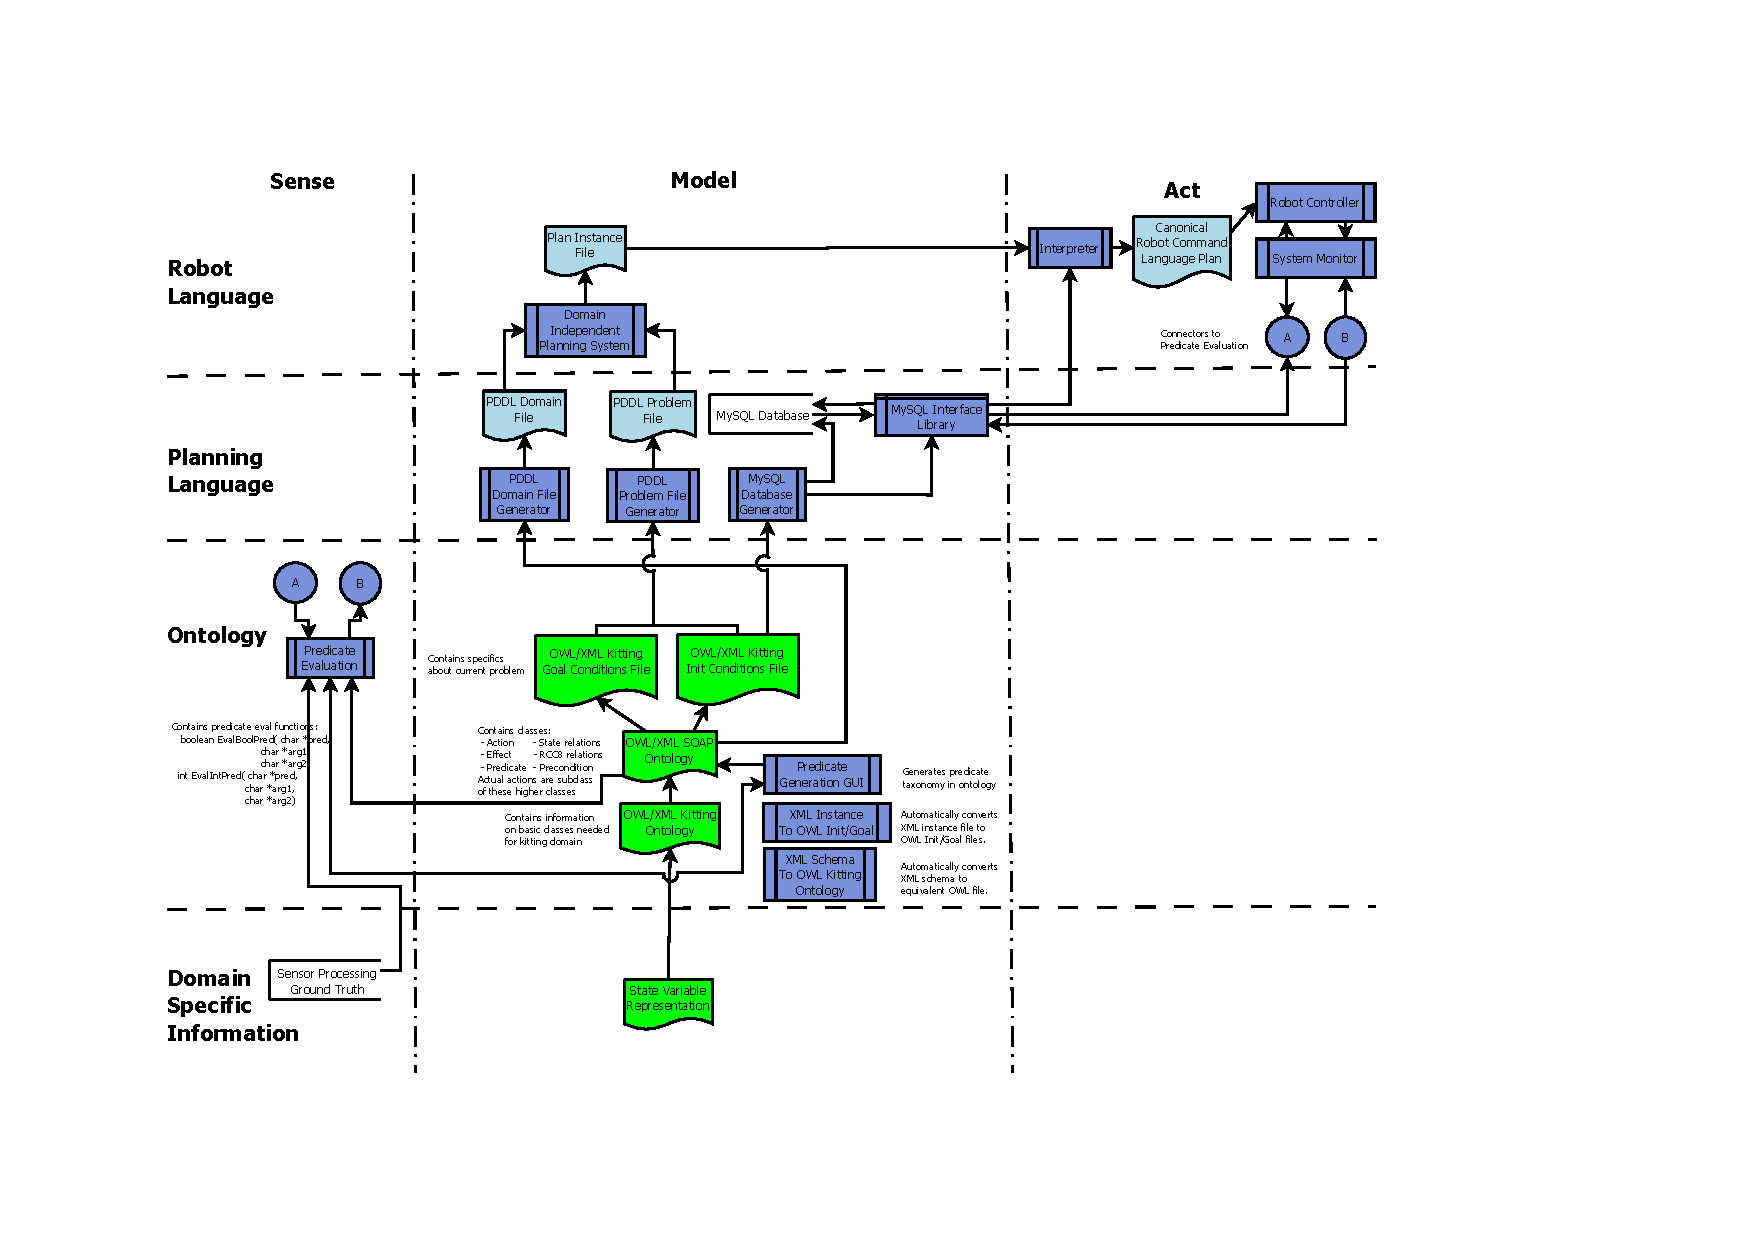
\includegraphics[width=13cm]{images/KnowledgeDrivenRobotics.pdf}
\caption{Knowledge Driven Design extensions- In this figure, green shaded boxes with curved bottoms
represent hand generated files while
light blue shaded boxes with curved bottoms represent automatically created boxes. Square
boxes represent processes and libraries.}
\label{fig:DesignArchitecture}
\end{center}
\end{figure}

The overall knowledge model of the system may be seen in Figure \ref{fig:DesignArchitecture}.
The figure is organized vertically by the representation that is used for the knowledge
and horizontally by the classical sense-model-act paradigm of intelligent systems.
On the vertical axis, knowledge begins with Domain Specific Information that captures
operational knowledge that is necessary to be successful in the particular domain in which
the system is designed to operate. This information is then organized into a domain
independent representation (an Ontology) that allows for the encoding of an object
taxonomy, object-to-object
relationships, and aspects of actions, preconditions, and effects.
Aspects of this
knowledge are automatically extracted and encoded in a form that is optimized for
a planning system to utilize (the Planning Language). Once a plan has been formulated,
the knowledge is transformed into a representation that is optimized for use by a robotic system
(the Robot Language).

It is acknowledged that sensing and action are important parts of a robotic system.
However, this article focuses on knowledge representation, and thus the modeling section
will be described in the most detail.

\subsection{Domain Specific Information}
The most basic knowledge that must be gathered for a knowledge
driven system is domain specific information (DSI). This appears along the bottom row of
Figure \ref{fig:DesignArchitecture}. DSI includes sensors and sensor processing that
are specifically tuned to operate in the target domain. Examples of sensor processing
may include pose determination and object identification.

For the knowledge model, a scenario driven approach is taken where
the DSI design begins with a domain expert creating one or more use cases and specific
scenarios that describe the typical operation of the system. Based on these scenarios and
use cases, the high-level
actions that the system must be able to accomplish can be enumerated and described.
An action description that includes any preconditions that
must be true for an action to be valid as well as expected effects that will result from a
given action is then created for each action.

\begin{figure}[ht!]
\begin{center}
\textsl{put-kittray}($\mathit{robot}$,$\mathit{kittray}$,$\mathit{worktable}$): The \textit{Robot}
$\mathit{robot}$ puts the \textit{KitTray} $\mathit{kittray}$ on the \textit{WorkTable} $\mathit{worktable}$.

\begin{tabular}{ l|l }
  \textit{preconditions} & \textit{effects} \\
  \hline
  \small {\textsf{kittray-location-robot}}(\small $\mathit{kittray}$,\small $\mathit{robot}$)
  &$\neg$\small {\textsf{kittray-location-robot}}(\small $\mathit{kittray}$,\small $\mathit{robot}$)\\
  \small {\textsf{robot-holds-kittray}}(\small $\mathit{robot}$,\small $\mathit{kittray}$)
  &$\neg$\small {\textsf{robot-holds-kittray}}(\small $\mathit{robot}$,\small $\mathit{kittray}$)\\
  \small {\textsf{worktable-empty}}(\small $\mathit{worktable}$)
  &$\neg$\small {\textsf{worktable-empty}}(\small $\mathit{worktable}$)\\
  &\small {\textsf{kittray-location-worktable}}(\small $\mathit{kittray}$,\small $\mathit{worktable}$)\\
  &\small {\textsf{robot-empty}}(\small $\mathit{robot}$)\\
  &\small {\textsf{on-worktable-kittray}}(\small $\mathit{worktable}$,\small $\mathit{kittray}$)\\
\end{tabular}
\caption{Example action along with its preconditions and expected effects.}
\label{fig:ActionExample}
\end{center}
\end{figure}

Based on the action description, objects in the environment that are relevant
for system operation can be identified. For example, the action depicted in Figure \ref{fig:ActionExample}
has a given robot place a kit tray onto a work table. The preconditions for this action are that
the robot is holding a kit tray and there is a clear space on the table to place the tray. This is
represented by the predicate expressions shown in Figure \ref{fig:ActionExample} that specify that
the robot is holding the kit tray, the kit tray is located on the robot (actually in its gripper), and
the work table is empty. The expected effects of this action are that the kit tray is now located
on the work table and the robot is no longer holding it. This is also represented by a series
of predicates that are shown in Figure \ref{fig:ActionExample}. Based on the preconditions and expected effects,
the objects that are relevant to this action include the robot, the kit tray, and the work table.
Aspects of these items may now be represented in the DSI. For example, that a kit tray has a location and may
be held by the robot or placed on the work table.

\subsection{Ontology}
The design transitions from domain expertise to knowledge modeling expertise
when the SVR is used to generate an ontology which consists of three parts:
\begin{enumerate}
 \item A base ontology that describes the objects in the scenario. This file contains
all of the basic information that was determined to be needed during the evaluation of
the use cases and scenarios. The knowledge is represented in as compact of a form as
possible with knowledge classes inheriting common attributes from parent classes.
For example, the class for a work table, \class{WorkTable} is derived from
\class{BoxyObject}, and \class{BoxyObject} is derived from \class{SolidObject}. The actual size of the work table
is defined in the \class{BoxyObject}. The \class{WorkTable} includes all of the attributes
of a \class{BoxyObject} along with the notion that a work table is something that can have
other objects placed on it. The work table itself is part of a work station \class{WorkStation}.
 \item Extensions that describe the States of the world and relationships between states,
Ordering constructs, Actions, and Predicates (the \onto{SOAP} ontology)
that are relevant to the scenario. This extension contains not only the basic class for
actions and predicates, but also the individual actions and predicates that are necessary
for the domain under study. In the case of the kit building domain, it was found that
10 actions and 16 predicates were necessary.
 \item Instance files that describe the initial and goal states for the system. The final set
of files for the ontology contain a description of the complete system starting or initial state and the
requirements on the goal state. The initial state file must contain a description of the environment that
is complete enough for a planning system to be able to create a valid sequence of actions that will achieve
the given goal state. For the kit building domain, this includes information such as the location of the
various end effectors that are available to the robot, the locations and contents of part supply bins, and
the location where finished kits should be placed. The goal state file only needs to contain information that
is relevant to the end goal of the system. For the case of building a kit, this may simply be that a complete
kit is located in a bin designed to hold completed kits.
\end{enumerate}
The ontology files are
described in more detail in Section \ref{Sect:Ontology}.

\subsection{Planning Language}
The Planning Domain Definition Language (PDDL) \cite{PDDL} is an attempt by the
domain independent planning community to formulate a standard language
for planning. A community of planning researchers has been producing
planning systems that comply with this formalism since the first International
Planning Competition held in 1998. This competition series continues today,
with the seventh competition being held in 2011. PDDL is constantly
adding extensions to the base language in order to represent more expressive
problem domains. The work represented in this article is based on PDDL Version 3.
By placing the knowledge in a PDDL representation, the use of an
entire family of open source planning systems is enabled.

The PDDL input format consists
of two files that specify the domain and the problem. As shown in Figure
\ref{fig:DesignArchitecture}, these files are automatically
generated from the ontology. The domain file represents actions along
with required preconditions and expected results. The problem file
represents the initial state of the system and the desired goal.

From these two files, a domain independent planning system such as
the forward-chaining partial-order planning from Coles et. al
\cite{Coles.ICAPS.2010} may be run to create a static plan file. This
plan file contains a sequence of actions that will transition the
system from the initial state to the goal state. It should be noted that
it is not possible for certain pieces of necessary data to be specified before
run time. For example the location of objects that are contained
in a random bin is necessary for them to be picked up by the robot,
however, this location will not be known before the bin has been examined.
To compensate for this lack of exact knowledge, the plans that are
generated by the PDDL planning system contain only high-level actions.

\begin{figure}[t!h!]
\begin{minipage}{.5\paperwidth}
\begin{list}{}{\setlength{\leftmargin}{1em}}\item\small
\begin{Verbatim}[commandchars=\\\{\},fontsize=\scriptsize, numbers=left, numbersep=2pt]
(attach-eff robot_1 tray_gripper tray_gripper_holder)
(take-kit-tray robot_1 kit_tray_1 empty_kit_tray_supply tray_gripper work_table_1)
(put-kit-tray robot_1 kit_tray_1 work_table_1)
(create-kit kit_a2b2c1 kit_tray_1 work_table_1)
(remove-eff robot_1 tray_gripper tray_gripper_holder)
(attach-eff robot_1 part_gripper part_gripper_holder)
(take-part robot_1 part_b_1 part_b_tray part_gripper work_table_1 kit_a2b2c1)
(put-part robot_1 part_b_1 kit_a2b2c1 work_table_1)
(take-part robot_1 part_a_1 part_a_tray part_gripper work_table_1 kit_a2b2c1)
(put-part robot_1 part_a_1 kit_a2b2c1 work_table_1)
...
(remove-eff robot_1 part_gripper part_gripper_holder)
(attach-eff robot_1 tray_gripper tray_gripper_holder)
(take-kit robot_1 kit_a2b2c1 work_table_1 tray_gripper)
(put-kit robot_1 kit_a2b2c1 finished_kit_receiver)
\end{Verbatim}
\end{list}
\end{minipage}
\caption{Excerpt of the PDDL solution file for kitting.}
\label{fig:domain}
\end{figure}
For example, the problem file will specify that a kit tray is located
on a work table. The exact position of the tray relative to the table
is not specified, nor is the location of the table relative to the global
origin of the world. Such detailed information must be gathered by sensor
processing, and the static PDDL problem file does not lend itself to well
to the storage of this information.

\subsection{Robot Language}
From this point forward, automatic planning tools have been designed to transition
the knowledge into a planning framework and finally a robot specific framework.

As such, it is assumed that a system has been implemented
that is capable of basic robotic actions. In our case, our knowledge
driven system bottoms out in a Robot Operating System (ROS) control layer
\footnote{Certain commercial/open source software and tools are identified
in this paper in order to explain our research. Such identification does not imply
recommendation or endorsement by the authors or NIST, nor does it
imply that the software tools identified are necessarily the best available for the purpose.}. 

\section{Industrial Kitting}
\label{Sect:Kitting}
\documentclass[letter,11pt,oneside]{article}
%%%%%%%%%%%%%%%%%%%%%%%%%%%%%%%%%%%%%%%%%%%%%%%%%%%%%%%%%%%%
%2345678901234567890123456789012345678901234567890123456789012345678901234567890
%        1         2         3         4         5         6         7         8

\documentclass[letterpaper, 10 pt, conference]{ieeeconf}  % Comment this line out
                                                          % if you need a4paper
%\documentclass[a4paper, 10pt, conference]{ieeeconf}      % Use this line for a4
                                                          % paper

\IEEEoverridecommandlockouts                              % This command is only
                                                          % needed if you want to
                                                          % use the \thanks command
\overrideIEEEmargins
% See the \addtolength command later in the file to balance the column lengths
% on the last page of the document



% The following packages can be found on http:\\www.ctan.org
%\usepackage{graphics} % for pdf, bitmapped graphics files
%\usepackage{epsfig} % for postscript graphics files
%\usepackage{mathptmx} % assumes new font selection scheme installed
%\usepackage{times} % assumes new font selection scheme installed
%\usepackage{amsmath} % assumes amsmath package installed
%\usepackage{amssymb}  % assumes amsmath package installed
\usepackage{graphicx}
\usepackage{verbatim}
\usepackage{multirow}
\usepackage{rotating}
\usepackage{moreverb}                    % for boxedboxedverbatim
\usepackage{array}
\usepackage{fancyvrb}
\usepackage{multicol}
\usepackage{mdwlist}
\usepackage{enumerate}
%\usepackage{tikz-er2}


\newtheorem{defn}{Definition}

\newcommand{\class}[1] {\textit{#1}}
\newcommand{\const}[1] {$\mathit{#1}$}
\newcommand{\objvar}[1] {$\mathsf{#1}$}
\newcommand{\stvar}[1] {\textsf{#1}}
\newcommand{\op}[1] {\textsl{#1}}
\newcommand{\nil} {\textit{nil}\ }

\newcommand\T{\rule{0pt}{2.6ex}}
\newcommand\B{\rule[-1.2ex]{0pt}{0pt}}

%\definecolor{violetred}{cmyk}{0,0.85,0.31,0.18}
%\definecolor{darkblue}{cmyk}{1,1,0,0.45}
%\definecolor{lavenderblush4}{cmyk}{0,0.06,0.04,0.45}
%\definecolor{packergreen}{cmyk}{0.46,0,0.21,0.76}
%\definecolor{fuschia}{cmyk}{0,100,0,0}
%\definecolor{graycmyk}{cmyk}{0,0,0,0.74}
%
%\usetikzlibrary{calc,trees,positioning,arrows,chains,shapes.geometric,%
%    decorations.pathreplacing,decorations.pathmorphing,shapes,%
%    matrix,shapes.symbols,positioning,shadows}
%
%% styles for flowcharts
%
%\tikzstyle{every entity} = [top color=white, bottom color=blue!30,
%                            draw=blue!50!black!100, drop shadow]
%\tikzstyle{empty} = [top color=white, bottom color=white,
%                            draw=white]
%
%\tikzstyle{every weak entity} = [drop shadow={shadow xshift=.7ex,
%                                 shadow yshift=-.7ex}]
%\tikzstyle{every attribute} = [top color=white, bottom color=green!20,
%                               draw=green, node distance=1cm, drop shadow]
%\tikzstyle{ELLIPSE} = [draw, ellipse, top color=white, bottom color=green!20, draw=green, drop shadow]
%\tikzstyle{MainAttribute} = [draw, rectangle,top color=white, bottom color=red!20,
%                               draw=red, node distance=1cm, drop shadow]
%\tikzstyle{DATABASE} = [draw, rectangle, rounded corners,top color=white, bottom color=graycmyk!50, draw=graycmyk, inner sep=10pt, drop shadow={shadow xshift=.7ex, shadow yshift=-.7ex}]
%
%
%\tikzstyle{myarrow}=[->, >=stealth', thick, shorten <=2pt,shorten >=2pt]
%
%
%
%\tikzstyle{output} = [draw, rectangle, rounded corners,top color=white, bottom color=red!30, draw=red, inner sep=10pt, drop shadow={shadow xshift=.7ex, shadow yshift=-.7ex}]
%
%\tikzstyle{abstract}=[rectangle, draw=black, rounded corners, fill=blue!40, drop shadow,
%        text centered, anchor=north, text=white, text width=3cm]
%
%
%\newbox{\LegendOutput}
%\savebox{\LegendOutput}{
%    (\begin{tikzpicture}[]
%    \node[output] (2) {\hspace{5 mm}};
%    \end{tikzpicture}
%    )}


\newenvironment{mylisting}
{\begin{list}{}{\setlength{\leftmargin}{1em}}\item\small}
{\end{list}}

\newenvironment{mytinylisting}
{\begin{list}{}{\setlength{\leftmargin}{1em}}\item\tiny\bfseries}
{\end{list}}


\title{\LARGE \bf
Metrics and Test Methods for Industrial Kit Building
}

%\author{ \parbox{3 in}{\centering Stephen Balakirsky\\
%         Intelligent Systems Division\\
%         National Institute of Standards and Technology\\
%        Gaithersburg, MD 20899, USA\\
%         {\tt\small stephen.balakirsky@nist.gov}}
%         \hspace*{ 0.5 in}
%         \parbox{3 in}{ \centering Zeid Kootbally\\
%          Department of Mechanical Engineering \\
%         University of Maryland\\
%         College Park, MD 20742, USA\\
%         {\tt\small zeid.kootbally@nist.gov}}\\ \\
%	\parbox{2.25 in}{\centering Craig Schlonoff\\
%         Intelligent Systems Division\\
%         National Institute of Standards and Technology\\
%        Gaithersburg, MD 20899, USA\\
%         {\tt\small craig.schlenoff@nist.gov}}
%        \hspace*{0.05in}
%         \parbox{2.25 in}{ \centering Thomas Kramer\\
%          Department of Mechanical Engineering \\
%         Catholic University of America\\
%         Washington, DC 20064, USA\\
%         {\tt\small thomas.kramer@nist.gov}}
%        \hspace*{0.05in}
%         \parbox{2.25 in}{ \centering Satyandra K. Gupta\\
%          Maryland Robotics Center\\
%         University of Maryland\\
%         College Park, MD 20742, USA\\
%         {\tt\small skgupta@umd.edu}}\\
%}

\author{Stephen Balakirsky, Thomas Kramer, and Zeid Kootbally% <-this % stops a space
\thanks{S. Balakirsky is with the Intelligent Systems Division, National Institute of Standards and Technology, Gaithersburg, MD, USA (e-mail:stephen.balakirsky@nist.gov)}% <-this % stops a space
\thanks{Z. Kootbally is with the Department of Mechanical Engineering, University of Maryland, College Park, MD, USA (email: zeid.kootbally@nist.gov)}%
\thanks{T. Kramer is with the Department of Mechanical Engineering, Catholic University of America, Washington, DC, USA (email: thomas.kramer@nist.gov)}%
} 

%%Filename:      EileenBl.fd
%Created by:    MLO
%Creation date: 2003/04/02

% This file should be put in a TeX input directory

\ProvidesFile{EileenBl.fd}
   [2003/04/02 Font definition file for U/EileenBl]

\DeclareFontFamily{U}{EileenBl}{}

\DeclareFontShape{U}{EileenBl}{xl}{n}{
   <-> EileenBl
}{}

\endinput

\begin{document}

%\author{Ze\"id KOOTBALLY}
\title{\centering Moving Object Predictions in Dynamic Environments for Autonomous Ground Vehicles\\
         ------\\
         Pr�diction des Positions de V�hicules Autonomes dans un Environnement Routier Dynamique
        }

\promotortitle{Promoters}
\promotor{Prof. \#1, Academy \#1\\
          Prof. \#2, Academy \#2\\
          Prof. \#3, Academy \#3\\
          Prof. \#4, Academy \#4\\
          Prof. \#5, Academy \#5\\
          Prof. \#6, Academy \#6}
\advisortitle{Advisors}
\advisors{Prof. Dr. Sebti Foufou, Universit\'e de Bourgogne\\
        Craig Schlenoff, National Institute of Standards and Technology (NIST)}



\faculty{UNIVERSIT\'E DE BOURGOGNE\\
U.F.R. SCIENCES ET TECHNIQUES} \department{} \reason{Th\`ese
pr\'esent\'ee par}
%\date{December \usefont{OT1}{phv}{mc}{n}\selectfont 12$\mathrm{^{th}}$, 2008}
\date{Soutenue le 12 d\'ecembre 2008}
\maketitlepage \cleardoublepage

%%%%%%%%%%%%%%%%%%%%%%%%%%%%%%%%%%%%%%%%%%%%%%%%%%%%%%%%%%%%%%%%%%%%%%%%%%%%%%%
%   Title Page                                                                %
%%%%%%%%%%%%%%%%%%%%%%%%%%%%%%%%%%%%%%%%%%%%%%%%%%%%%%%%%%%%%%%%%%%%%%%%%%%%%%%
\begin{titlepage}
\begin{center}

%\vspace{1.5cm} %
%\large{M\'emoire pr\'esent\'e par}\\
%\LARGE{\textbf{Ze\"id Kootbally}}\\
%\large{en vue de l'obtention}\\
%\LARGE{\textbf{d'une th\`ese de doctorat en Informatique}}\\
%\LARGE{\textbf{de l'Universit\'e de Bourgogne - Dijon}}\\

\vspace{1.5cm} %
\rule[1ex]{1\textwidth}{0.3mm} \\%
\huge{\textbf{A Literature Review of Robot Agility Methods, Use Cases, and Metrics for Manufacturing Assembly Applications}}\\
%\huge{------}\\
%\huge{\textbf{Moving Object Predictions in Dynamic Environments for Autonomous Ground Vehicles}}\\
\rule[1ex]{1\textwidth}{0.3mm} \\%

\vspace{1.5cm} %
%\large{Soutenue publiquement le xxx devant le jury compose de~:}\\

\vspace{1.5cm} %
\begin{small}
\begin{tabular}{p{3.8cm}p{7.5cm}l}
%\begin{tabular}{lll}
Zeid Kootbally & University of Maryland  &  \\
Andrew Price & Georgia Institute of Technology  &  \\
Henrik Christensen & Georgia Institute of Technology  &  \\
Stephen Balakirsky & Georgia Institute of Technology  & \\
Anthony Downs & National Institute of Standards and Technology  &  \\
Craig Schlenoff & National Institute of Standards and Technology  & \\
\end{tabular}
\end{small}
\end{center}
\end{titlepage}
\cleardoublepage

\pagenumbering{roman} 
%\include{Chapters/abstract-english}
%\cleardoublepage
%\include{Chapters/abstract-french}
%\cleardoublepage

%\include{Chapters/dedication}
%\cleardoublepage
\markboth{Contents}{Contents}
\tableofcontents
\cleardoublepage

\pagenumbering{arabic}
\section{Introduction}
A failure is any change, design, or manufacturing error that renders a component, assembly, or system incapable of performing its intended function \cite{Collins93}. In kitting, as described in Section \ref{sect:kitting}, failures can occur for multiple reasons that include equipment not being set up properly, tools and/or fixtures not being properly prepared, and improper equipment maintenance. Part/component availability failures can be triggered by inaccurate information on the location of the part, part damage, incorrect part types, or part shortage due to delays in internal logistics. In order to prevent or minimize failures, a disciplined approach needs to be implemented to identify the different ways a process design can fail before impacting productivity.

Even though today's state-of-the-art industrial robots are capable of sub-millimeter accuracy \cite{RobotAccuracy}, they often lack the sensing
necessary to detect failures and the programming required to cope with and correct the failure. This is due to the fact that they are often programmed
by an operator using crude positional controls from a teach pendant. These teach pendant programs are highly repeatable, which provides 
utility for large-batch, error-free operation. However, the cyclic program that repeats identical operations does not lend itself well to adaptation for 
failure mitigation. In fact, producing a program to correct a perceived failure would require that the cell be taken off-line
for additional human-led teach pendant programming. In addition, 
most cells lack the ability to sense that a failure occurred and  lack programming (that would have had to be teach pendant entered) to cope
with failure conditions, thus making it impossible for the cell to recover from failures.
This leads to faulty products being sent down the line, and/or downtime for the cell as failures are detected and corrected.

For small batch processors or other customers who must frequently change their line configuration or desire to perform complex operations
with their robots, this frequent downtime and lack of failure correction/detection may be unacceptable. The robotic systems of tomorrow need to be capable, flexible, and agile.  
These systems need to perform their duties at least  as well as human counterparts, be quickly re-tasked to other operations, cope with a wide 
variety of unexpected environmental and operational changes, and be able to detect and correct errors in operation. 
To be successful, these systems need to combine domain expertise, knowledge of their own skills and limitations, and both semantic and geometric 
environmental information.

The IEEE Robotics and Automation Society's Ontologies for Robotics and Automation Working Group has taken the first steps in creating the 
infrastructure necessary for such a system, while the Industrial Subgroup has applied this infrastructure to create a sample kit building
system.  This work is presented in Balakirsky et al. \cite{balakirsky2013} which describes the construction of a robotic kit building
system that is able to cope with environmental and task changes without operator intervention. This article extends that work to utilize
the same infrastructure to allow for the detection and correction of action failures in the system.

The organization of the remainder of this paper is as follows. Section \ref{sect:kitting} describes the domain of kit building. Section \ref{sect:overview} presents
an overview of the software system architecture as well as details of the ontology and world model for the robot cell. Section \ref{sect:operation} discusses the detailed operation of cell, and Section \ref{sect:failure} discusses how failures are handled by the ontology. Finally, Section \ref{sect:future} presents
conclusions and future work.
%
%
\section{Kitting}
\label{sect:kitting}
Today's advanced manufacturing plants utilize mixed-model assembly where multiple product variants are built on the same line.  
According to Jim Tetreault, Ford’s vice president of North America Manufacturing, 
new Ford assembly facilities are able to build a full spectrum of vehicles on the same assembly line \cite{James2011}. One of the technologies that makes this possible
is the use of assembly kits.  Bozer and McGinnis \cite{Bozer1992} describe a kit as ``a specific
collection of components and/or subassemblies that together (i.e., in the same container) support one or more assembly
operations for a given product or shop order''. These  kits provide a synchronous material flow, where parts and components move to 
assembly stations in a just-in-time manner. The kits provide workers with the parts and tools that they need (which may vary from 
vehicle model to vehicle model) in the sequence that they need them. The use of kitting also allows a single delivery system to feed
multiple assembly stations thus saving manufacturing or assembly space \cite{Medbo2003} and provides an additional inspection opportunity 
that allows for the detection of part defects before they impact assembly operations. The individual operations of the station 
that builds the kits may be viewed as a specialization of the general
bin-picking problem \cite{Schyja2012} where parts are picked from one or more part bins or trays and placed into specific slots in a kit tray.

For our sample implementation, we assume that the robot cell is building one of several possible kit configurations. At execution time, the
cell has a set kit to build, but does not know the precise location of the kit tray, the part trays, or the location of individual parts in the part tray.
When a human builds a kit, they are able to inspect each part before adding it to the kit tray. This provides an additional level of quality control and
is an aspect that is desirable to have in our robotic system. During kit construction,
a robot performs a series of pick-and-place operations
in order to construct the kit. These operations include:
\begin{enumerate}
\item Pick up an empty kit and place it on the work table.
\item Pick up multiple component parts, inspect them, and place them in the kit.
\item Pick up the completed kit and place it in the full kit storage area.
\end{enumerate}
Each of these steps may be a compound action that includes
other actions such as end-of-arm tool changes, path planning,
and obstacle avoidance. The items that are being placed in the kit may be of varying size and shape and have various grasping and inspection
requirements.
%
\begin{figure}[htb!]
\begin{center}
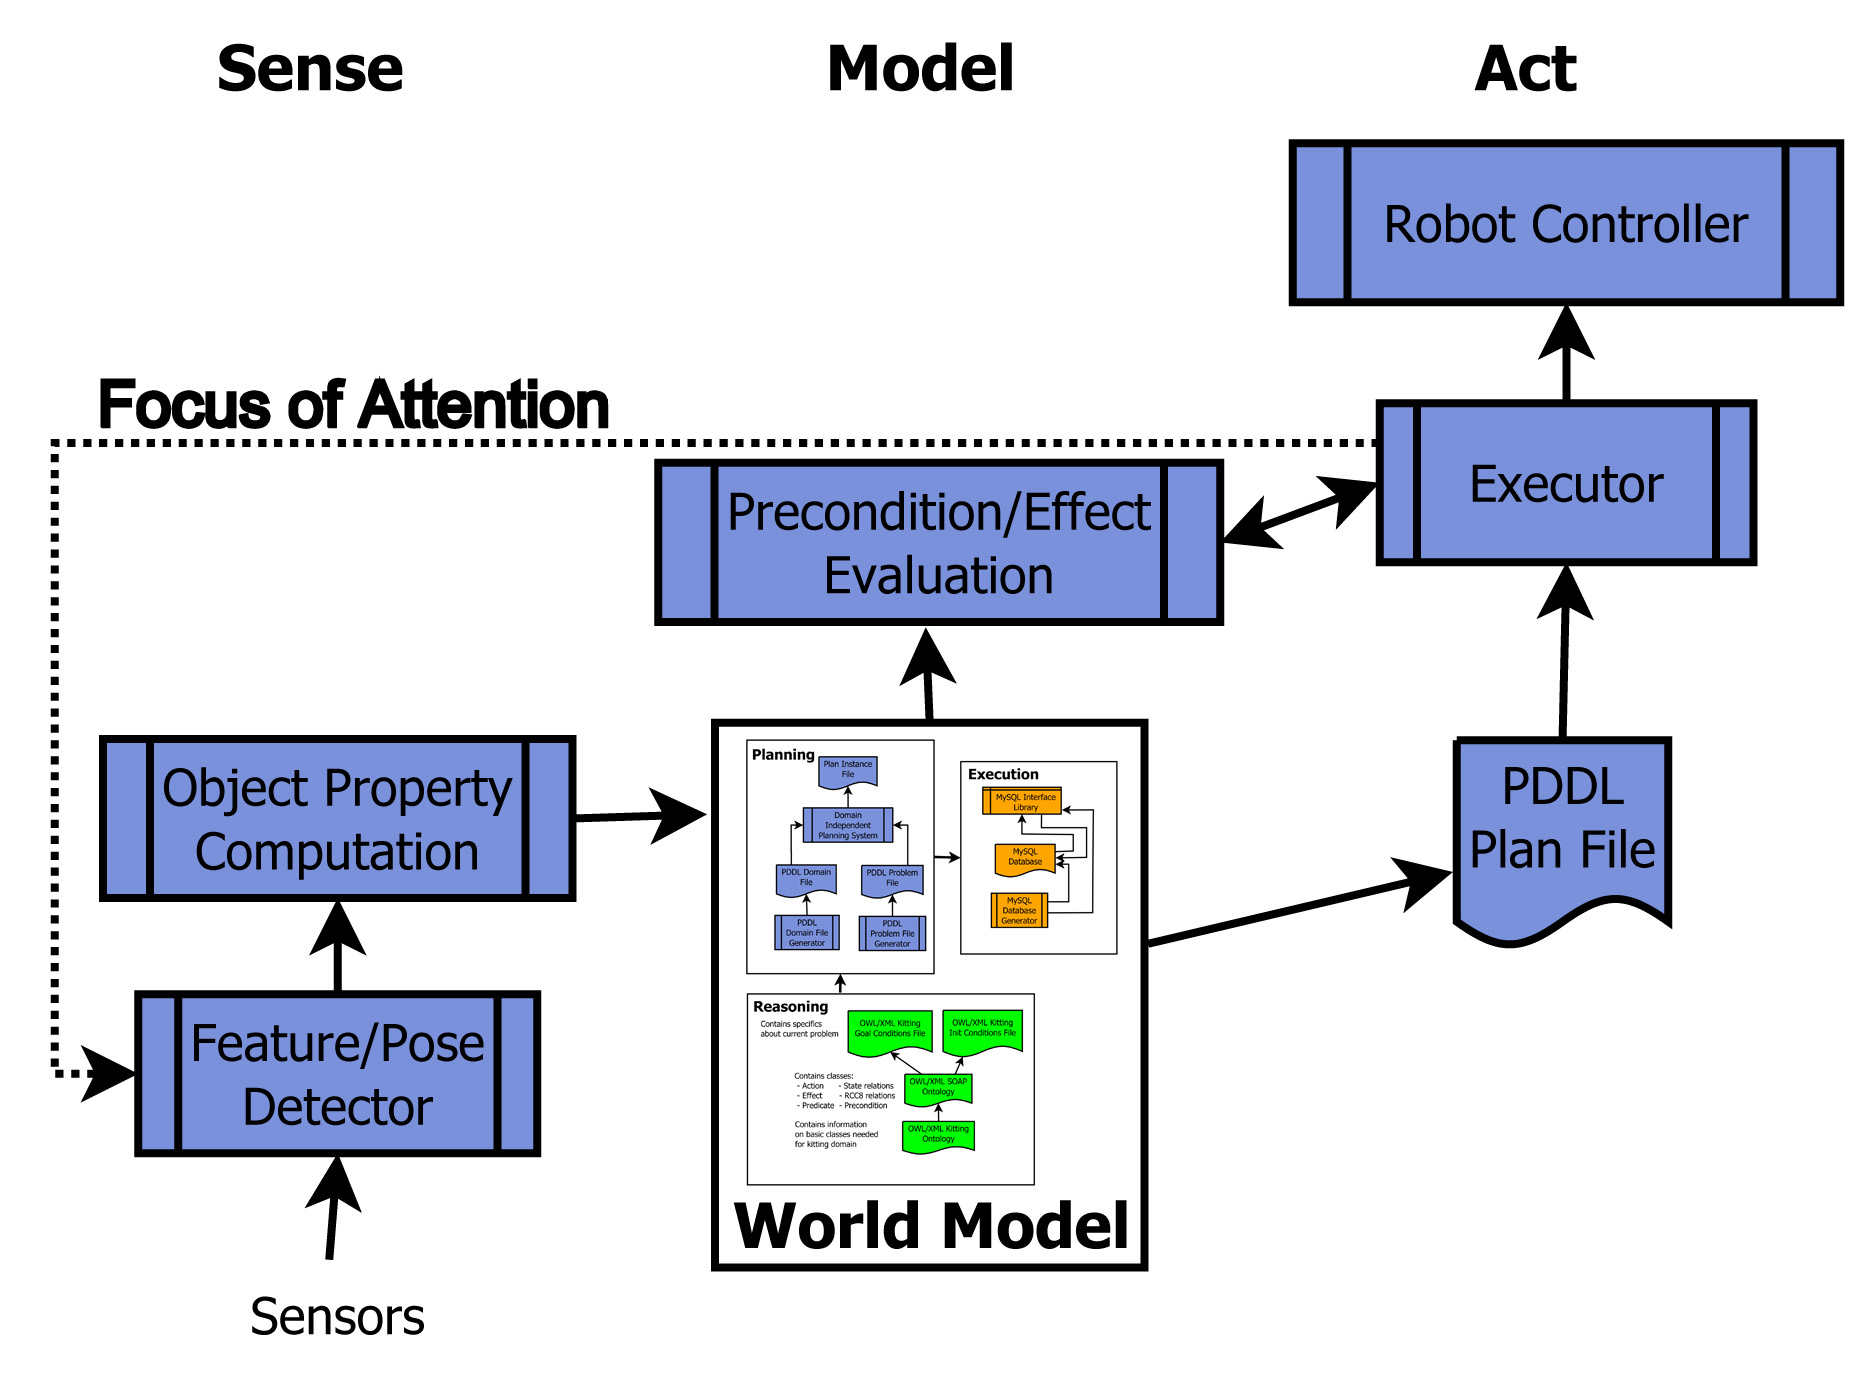
\includegraphics[width=8.5cm]{images/RITAExecution.jpg}
\caption{Major components that make up the Sense--Model--Act paradigm of the kitting station.}
\label{fig:SenseModelAct}
\end{center}
\end{figure}
\section{Domain Specific Information}\label{kitting_domain}

The foundation for the knowledge representation is domain specific information that is produced by an expert in the particular field of study. This includes
information on items ranging from what actions and attributes are relevant, to what the necessary conditions are for an action to occur and what the
likely results of the action are. We have chosen to encode this basic information in a formalism know as a state variable representation (SVR) \cite{NAU.2004}.
This information will then flow up the abstraction and be transformed into the ontology, planning language, and robot language.\\
Before building a SVR, the domain for kitting needs to be specified. The domain for kitting contains some fixed equipment: a robot, a work table, end effectors, end effector holders, and an end effector changing station. Items that enter the workstation include kit trays, boxes in which to put kits, boxes that contain empty kit trays, and part supplies. Items that leave the workstation may be boxes with finished kits inside, empty part trays, empty boxes. An external agent is responsible of moving the items that leave the workstation. We assume that the workstation has only one work table, one changing station, and one robot.

%\section{State-Variable Representation}


In a State Variable Representation (SVR), each state is represented by a tuple of values of $n$ state variables $\lbrace x_1,\dots,x_n\rbrace$, and each action is represented by a partial function that maps this tuple into some other tuple of values of the $n$ state variables.\\ \\
To build the SVR, the group has taken a very systematic approach of identifying and modeling the concepts. Because the industrial robot field is so broad, the group decided to limit its efforts to a single type of operation, namely kitting. A scenario was developed that described, in detail, the types of operations that would be performed in kitting, the sequencing of steps, the parts and machines that were needed, constraints on the process such as pre- and post-conditions, etc. For this scenario, a set of concepts were extracted and defined. These concepts served as the initial requirements for the kitting SVR. The concepts were then modeling in our SVR, building off of the definitions and relationships that were identified in the scenario. A SVR relies on the elements of constant variable symbols, object variable symbols, state variable symbols, and planning operators. These are defined for the kitting domain in the rest of this section.


\subsection{Constant Variable Symbols}
For the kitting domain, there is a finite set of constant variable symbols that must be represented. In the SVR, constant variable symbols are partitioned into disjoint classes corresponding to the objects of the domain. The finite set of all constant variable symbols in the kitting domain is partitioned into the following sets:
%\begin{small}
\begin{itemize}
\item A set of \class{Part}: A \class{Part} is the basic item that will be used to fill a kit.

\item A set of \class{PartsTray}: \class{Parts} arrive at the workstation in \class{PartsTrays}. Each \class{Part} is at a known position in the \class{PartsTray}. Each \class{PartsTray} contains one type of \class{Part}.

\item A set of \class{KitTray}:  A \class{KitTray} can hold \class{Parts} in known positions.

\item A set of \class{Kit}: A \class{Kit} consists of a \class{KitTray} and, possibly, some \class{Parts}. A \class{Kit} is empty when it does not contain any \class{Part} and finished when it contains all the \class{Parts} that constitute a kit.

\item A set of \class{WorkTable}: A \class{WorkTable} is an area in the kitting workstation where \class{KitTrays} are placed to build \class{Kits}.

\item A set of \class{LargeBoxWithKits}: A \class{LargeBoxWithKits} contains only finished \class{Kits}.

\item A set of \class{LargeBoxWithEmptyKitTrays}: A \class{LargeBoxWithEmptyKitTrays} is a box that contains only empty \class{KitTrays}.

\item A set of \class{Robot} \{\const{robot\_1},\const{robot\_2},\ldots\}: A \class{Robot} in the kitting workstation is a robotic arm that can move objects in order to build \class{Kits}.

\item A set of \class{EndEffector}: \class{EndEffectors} are used in a kitting workstation to manipulate \class{Parts}, \class{PartsTrays}, \class{KitTrays}, and \class{Kits}. An \class{EndEffector} is attached to a \class{Robot} in order to grasp objects.

\item A set of \class{EndEffHolder}: An \class{EndEffHolder} is a storage unit that holds one type of \class{EndEffector}.

\item A set of \class{EndEffChStation}: An \class{EndEffChStation} is made up of \class{EndEffHolders}.
\end{itemize}
%\end {small}

\subsection{Object Variable Symbols}
Object variable symbols are typed variables which range over a class or the union of classes of constant variable symbols. Examples of object variable symbols are \const{r} $\in$ \class{Robots}, \const{kt} $\in$ \class{KitTrays}, etc.

\subsection{State Variable Symbols}
\label{subsect:State_Variable_Symbols}
A state variable symbol is defined as follows:\\
$\mathrm{x: A_1\times \dots\times A_i\times S\rightarrow}$ $\mathrm{B_1\cup\dots\cup B_j}$ $\cup$ \textit{bool} $\cup$ \textit{\{\}} $\cup$ \textit{numeric} ($i, j\geq 1$) is a function from the set of states ($\mathrm{S}$) and at least one set of constant variable symbols $\mathrm{A_1\times \dots\times A_i}$ into a set $\mathrm{B_1\cup\dots\cup B_j}$ $\cup$ \textit{bool} $\cup$ \textit{\{\}} $\cup$ \textit{numeric} where:

\begin{itemize}
\item $\mathrm{B_1\cup\dots\cup B_j}$ is a set of constant variable symbols
\item \textit{bool} is a boolean
\item \{\} is an empty set
\item \textit{numeric} is a numerical value
\end{itemize}

\noindent
The use of state variable symbols reduces the possibility of inconsistent states and generates a smaller state space. The following state variable symbols are used in the kitting domain.

\begin{itemize}
\item \stvar{endeff-location}\\ \class{EndEffector}$\mathrm{\times S\rightarrow}$\class{Robot} $\cup$ \class{EndEffHolder}: designates the location of an \class{EndEffector} in the workstation. An \class{EndEffector} is either attached to a \class{Robot} or placed in an \class{EndEffHolder}.

\item \stvar{robot-with-endeff}\\ \class{Robot}$\mathrm{\times S\rightarrow}$\class{EndEffector} $\cup$ \{\}: designates the \class{EndEffector} attached to a \class{Robot} if there is one attached, otherwise nothing.

\item \stvar{on-wtable}\\ \class{WorkTable}$\mathrm{\times S\rightarrow}$\class{Kit} $\cup$ \class{KitTray} $\cup$ \{\}: designates the object placed on the \class{WorkTable}, i.e., a \class{Kit}, a \class{KitTray}, or nothing.

\item \stvar{kit-location}\\ \class{Kit}$\mathrm{\times S\rightarrow}$\class{LargeBoxWithKits} $\cup$ \class{WorkTable} $\cup$ \class{Robot}: designates the different possible locations of a \class{Kit} in the workstation, i.e., in a \class{LargeBoxWithKits}, on the \class{WorkTable}, or being held by a \class{Robot}.

\item \stvar{kittray-location}\\ \class{KitTray}$\mathrm{\times S\rightarrow}$\class{LargeBoxWithEmptyKitTrays} $\cup$ \class{WorkTable} $\cup$ \class{Robot}: designates the different possible locations of a \class{KitTray} in the workstation, i.e., in a \class{LargeBoxWithEmptyKitTrays}, on a \class{WorkTable} or being held by a \class{Robot}.

\item \stvar{part-location}\\ \class{Part}$\mathrm{\times S\rightarrow}$\class{PartsTray} $\cup$ \class{Kit} $\cup$ \class{Robot}: designates the different possible locations of a \class{Part} in the workstation, i.e., in a \class{PartsTray}, in a \class{Kit}, or being held by a \class{Robot}.

\item \stvar{robot-holds}\\ \class{Robot}$\mathrm{\times S\rightarrow}$\class{KitTray} $\cup$ \class{Kit} $\cup$ \class{Part} $\cup$ \{\}: designates the object being held by a \class{Robot}, i.e., a \class{KitTray}, a \class{Kit}, a \class{Part}, or nothing. It is assumed that the \class{Robot} is already equipped with the appropriate \class{EndEffector}.

\item \stvar{lbwk-full}\\ \class{LargeBoxWithKits}$\mathrm{\times S\rightarrow}$ \textit{bool}: designates if a \class{LargeBoxWithKits} is full or not.

\item \stvar{lbwekt-empty}\\ \class{LargeBoxWithEmptyKitTrays}$\mathrm{\times S\rightarrow}$ \textit{bool}: designates if a \class{LargeBoxWithEmptyKitTrays} is empty or not.

\item \stvar{partstray-empty}\\ \class{PartsTray}$\mathrm{\times S\rightarrow}$ \textit{bool}: designates if a \class{PartsTray} is empty or not.

\item \stvar{endffector-type}\\ \class{EndEffector}$\mathrm{\times S \rightarrow}$\class{KitTray} $\cup$ \class{Kit} $\cup$ \class{Part}: designates the type of object an \class{EndEffector} can hold, i.e., a \class{KitTray}, a \class{Kit}, or a \class{Part}.

\item \stvar{endeffholder-holds-endeff}\\ \class{EndEffHolder}$\mathrm{\times S \rightarrow}$\class{EndEffector} $\cup$ \{\}: designates wether an \class{EndEffHolder} is holding an \class{EndEffector} or nothing.

\item \stvar{endeffholder-location}\\ \class{EndEffHolder}$\mathrm{\times S \rightarrow}$\class{EndEffChStation}: designates the \class{EndEffChStation} where the \class{EndEffHolder} is located.

\item \stvar{endeffchstation-has-endeffholder}\\ \class{EndEffChStation}$\mathrm{\times S \rightarrow}$\class{EndEffHolder}: designates the \class{EndEffHolder} the \class{EndEffChStation} contains.

\item \stvar{found-part}\\ \class{PartsTray}$\mathrm{\times S \rightarrow}$\class{Part} $\cup$ \{\}: designates wether a \class{Part} is found in a \class{PartsTray} or not.

\item \stvar{origin-part}\\ \class{Part}$\mathrm{\times S \rightarrow}$\class{PartsTray}: designates the \class{PartsTray} where the \class{Part} is found.

\item \stvar{quantity-parts-in-partstray}\\ \class{PartsTray}$\mathrm{\times S \rightarrow}$\textit{numeric}: designates the number of parts that \class{PartsTray} contains.

\item \stvar{quantity-parts-in-kit}\\ \class{Kit}$\mathrm{\times}$\class{PartsTray}$\mathrm{\times S \rightarrow}$\textit{numeric}: designates the number of parts from \class{PartsTray} that \class{Kit} contains.

\item \stvar{capacity-parts-in-kit}\\ \class{Kit}$\mathrm{\times}$\class{PartsTray}$\mathrm{\times S \rightarrow}$\textit{numeric}: designates the number of parts from \class{PartsTray} that \class{Kit} \textbf{can} contain.

\end{itemize}


%\subsection{Rigid Relations}
%\label{subsubsect:Rigid_Relation}
%\stvar{efftype} and \stvar{effhold-eff} are rigid relations since their values do not vary from one state to another. In each state, a given \class{EndEffector} will %always hold the same type of object and a given \class{EndEffHolder} will always hold the same \class{EndEffectors}.

\subsection{Predicates and Functions}
In PDDL, predicates are used to encode Boolean state variables, while functions are used to model updates of numerical values~\cite{FOXandLong.2003}. This section describes the predicates and functions derived from the state variables described in section~\ref{subsect:State_Variable_Symbols}. We recall the following definition of a state variable ((section~\ref{subsect:State_Variable_Symbols})) $\mathrm{x: A_1\times \dots\times A_i\times S\rightarrow B_1\cup\dots\cup B_j}$ ($i, j\geq 1$) that is used to convert state variables into predicates as follows:

\begin{itemize}
 \item $\mathrm{A_1\times \dots\times A_i\times S\rightarrow B_1\cup\dots\cup B_j}$ ($i, j\geq 1$)
  \begin{itemize}
  \item \stvar{predicate\_1}($\mathcal{A,B}$)
  \item \ldots
  \item \stvar{predicate\_n}($\mathcal{A,B}$)
  \end{itemize}
\end{itemize}

Where $\mathcal{A} \in \mathrm{\{A_1,\ldots,A_i\}}$ and $\mathcal{B} \in \mathrm{\{B_1,\ldots,B_i\}}$ ($i, j\geq 1$)

\subsubsection{Predicates}



The state variables in our current kitting domain contains the following predicates.
\begin{itemize}
 \item \stvar{endeff-location}
  \begin{itemize}
  \item \stvar{endeff-location-robot}(\class{EndEffector},\class{Robot}) ;TRUE iff \class{EndEffector} is attached to \class{Robot}
  \item \stvar{endeff-location-endeffholder}(\class{EndEffector},\class{EndEffHolder}) ;TRUE iff \class{EndEffector} is in \class{EndEffHolder}
  \end{itemize}

 \item \stvar{robot-with-endeff}
  \begin{itemize}
  \item \stvar{robot-with-endeff}(\class{Robot},\class{EndEffector}) ;TRUE iff \class{Robot} is equipped with \class{EndEffector}
  \item \stvar{robot-with-no-endeff}(\class{Robot}) ;TRUE iff \class{Robot} is not equipped with any \class{EndEffector}	
  \end{itemize}

 \item \stvar{on-wtable}
  \begin{itemize}
  \item \stvar{on-wtable-kit}(\class{WorkTable},\class{Kit}) ;TRUE iff \class{Kit} is on the \class{WorkTable}
  \item \stvar{on-wtable-kittray}(\class{WorkTable},\class{KitTray}) ;TRUE iff \class{KitTray} is on the \class{WorkTable}
  \item \stvar{worktable-empty}(\class{WorkTable}) ;TRUE iff there is nothing on the \class{WorkTable}
  \end{itemize}

 \item \stvar{kit-location}
  \begin{itemize}
  \item \stvar{kit-location-lbwk}(\class{Kit},\class{LargeBoxWithKits}) ;TRUE iff \class{Kit} is in the \class{LargeBoxWithKits}
  \item \stvar{kit-location-wtable}(\class{Kit},\class{WorkTable}) ;TRUE iff \class{Kit} is on the \class{WorkTable}
  \item \stvar{kit-location-robot}(\class{Kit},\class{Robot}) ;TRUE iff \class{Kit} is being held by the \class{Robot}	
  \end{itemize}

 \item \stvar{kittray-location}
  \begin{itemize}
  \item \stvar{kittray-location-lbwekt}(\class{KitTray},\class{LargeBoxWithEmptyKitTrays}) ;TRUE iff \class{KitTray} is in the \class{LargeBoxWithEmptyKitTrays}	
  \item \stvar{kittray-location-robot}(\class{KitTray},\class{Robot}) ;TRUE iff \class{KitTray} is being held by the \class{Robot}
  \item \stvar{kittray-location-wtable}(\class{KitTray},\class{WorkTable}) ;TRUE iff \class{KitTray} is on the \class{WorkTable}
  \end{itemize}

 \item \stvar{part-location}
  \begin{itemize}
    \item \stvar{part-location-partstray}(\class{Part},\class{PartsTray}) ;TRUE iff \class{Part} is in the \class{PartsTray}	
    \item \stvar{part-location-kit}(\class{Part},\class{Kit}) ;TRUE iff \class{Part} is in the \class{Kit}
    \item \stvar{part-location-robot}(\class{Part},\class{Robot}) ;TRUE iff \class{Part} is being held by the \class{Robot}
  \end{itemize}

 \item \stvar{robot-holds}
  \begin{itemize}
    \item \stvar{robot-holds-kittray}(\class{Robot},\class{KitTray}) ;TRUE iff \class{Robot} is holding a \class{KitTray}	
    \item \stvar{robot-holds-kit}(\class{Robot},\class{Kit}) ;TRUE iff \class{Robot} is holding a \class{Kit}
    \item \stvar{robot-holds-part}(\class{Robot},\class{Part}) ;TRUE iff \class{Robot} is holding a \class{Part}
    \item \stvar{robot-empty}(\class{Robot}) ;TRUE iff \class{Robot} is not holding anything
  \end{itemize}

 \item \stvar{lbwk-full}
  \begin{itemize}
    \item \stvar{lbwk-not-full}(\class{LargeBoxWithKits}) ;TRUE iff \class{LargeBoxWithKits} is not full	
  \end{itemize}

 \item \stvar{lbwekt-empty}
  \begin{itemize}
    \item \stvar{lbwekt-not-empty}(\class{LargeBoxWithEmptyKitTrays}) ;TRUE iff \class{LargeBoxWithEmptyKitTrays} is not empty
  \end{itemize}

 \item \stvar{partstray-empty}
  \begin{itemize}
    \item \stvar{partstray-not-empty}(\class{PartsTray}) ;TRUE iff \class{PartsTray} is not empty
  \end{itemize}

 \item \stvar{endeff-type}
  \begin{itemize}
    \item \stvar{endeff-type-kittray}(\class{EndEffector},\class{KitTray}) ;TRUE iff \class{EndEffector} is capable of holding a \class{KitTray}	
    \item \stvar{endeff-type-kit}(\class{EndEffector},\class{Kit}) ;TRUE iff \class{EndEffector} is capable of holding a \class{Kit}
    \item \stvar{endeff-type-part}(\class{EndEffector},\class{Part}) ;TRUE iff \class{EndEffector} is capable of holding a \class{Part}
  \end{itemize}

 \item \stvar{endeffholder-holds-endeff}
  \begin{itemize}
    \item \stvar{endeffholder-holds-endeff}(\class{EndEffHolder},\class{EndEffector}) ;TRUE iff \class{EndEffHolder} is holding \class{EndEffector}
    \item \stvar{endeffholder-empty}(\class{EndEffHolder}) ;TRUE iff \class{EndEffHolder} is empty (not holding an \class{EndEffector})
  \end{itemize}


 \item \stvar{endeffholder-location}
  \begin{itemize}
    \item \stvar{endeffholder-location}(\class{EndEffHolder},\class{EndEffChStation}) ;TRUE iff \class{EndEffHolder} is in \class{EndEffChStation}
  \end{itemize}

\item \stvar{endeffchstation-has-endeffholder}
  \begin{itemize}
    \item \stvar{endeffchstation-has-endeffholder}(\class{EndEffChStation},\class{EndEffHolder}) ;TRUE iff \class{EndEffChStation} contains \class{EndEffHolder}
  \end{itemize}

\item \stvar{found-part}
  \begin{itemize}
    \item \stvar{found-part}(\class{Part},\class{PartsTray}) ;TRUE iff \class{Part} is found in \class{PartsTray}
  \end{itemize}

\item \stvar{origin-part}
  \begin{itemize}
    \item \stvar{origin-part}(\class{Part},\class{PartsTray}) ;TRUE iff \class{Part} is from \class{PartsTray}.
  \end{itemize}
\end{itemize}

\subsubsection{Functions}
In a planning model, numeric fluents represent function symbols that can take an infinite
set of values. Introducing functions into planning not only makes it possible to deal with numerical
values in a more general way than allowed for by a purely relational language but makes it possible to model operators in a more compact and sometimes also more natural way. The state variables in our current kitting domain contains the following functions.

\begin{itemize}
 \item \stvar{quantity-parts-in-partstray}
  \begin{itemize}
   \item \stvar{quantity-parts-in-partstray}(\class{PartsTray}) ;Quantity of parts in \class{PartsTray}
  \end{itemize}

 \item \stvar{quantity-parts-in-kit}
  \begin{itemize}
   \item \stvar{quantity-parts-in-kit}(\class{Kit},\class{PartsTray}) ;Quantity of parts from \class{PartsTray} that is in \class{Kit}
  \end{itemize}

     \item \stvar{capacity-parts-in-kit}
  \begin{itemize}
  \item \stvar{capacity-parts-in-kit}(\class{Kit},\class{PartsTray}) ;Quantity of parts from \class{PartsTray} that \class{Kit} \textbf{can} contain
  \end{itemize}
\end{itemize}


\subsection{Planning Operators and Actions}
\label{subsect:Planning_Operators}
The planning operators presented in this section are expressed in classical representation instead of state variable representation. In classical representation, states are represented as sets of logical atoms (predicates) that are true or false within some interpretation. Actions are represented by planning operators that change the truth values of these atoms.


\subsubsection{Planning Operators}
 In classical planning, a planning operator~\cite{NAU.2004} is a triple o=(\op{name}(o), \textit{preconditions}(o), \textit{effects}(o)) whose elements are as follows:
\begin{itemize}
\item \op{name}(o) is a syntactic expression of the form $n(x_1,\dots,x_k)$, where $n$ is a symbol
called an operator symbol, $x_1,\dots,x_k$ are all of the object variable symbols that
appear anywhere in \textit{o}, and $n$ is unique (i.e., no two operators can have the
same operator symbol).
\item \textit{preconditions}(o) and \textit{effects}(o) are sets of literals (i.e., atoms and negations of atoms). Literals that are true in \textit{preconditions}(o) but false in \textit{effects}(o) are removed by using negations of the appropriate atoms.
\end{itemize}

Our kitting domain is composed of ten operators which are defined below.


\begin{enumerate}

%%%%%%%%%%%%%%%%%%%%%%%%%%%%%%%%%%%%% take-kittray
\item \op{take-kittray}(\const{robot},\const{kittray},\const{lbwekt},\const{endeff},\const{worktable}): The \class{Robot} \const{robot} equipped with the \class{EndEffector} \const{endeff} picks up the \class{KitTray} \const{kittray} from the \class{LargeBoxWithEmptyKitTrays} \const{lbwekt}.


\begin{tabular}{ l|l }
  \textit{preconditions} & \textit{effects} \\
  \hline
  \stvarsmall{robot-empty}(\constsmall{robot})&$\neg$\stvarsmall{robot-empty}(\constsmall{robot})\\
  \stvarsmall{kittray-location-lbwekt}(\constsmall{kittray},\constsmall{lbwekt})&$\neg$\stvarsmall{kittray-location-lbwekt}(\constsmall{kittray},\constsmall{lbwekt}) \\
  \stvarsmall{lbwekt-not-empty}(\const{lbwekt})&\stvarsmall{kittray-location-robot}(\constsmall{kittray},\constsmall{robot})\\
  \stvarsmall{robot-with-endeff}(\const{robot},\constsmall{endeff})&\stvarsmall{robot-holds-kittray}(\constsmall{robot},\constsmall{kittray}) \\

  \stvarsmall{endeff-location-robot}(\constsmall{endeff},\constsmall{robot})&\\
  \stvarsmall{worktable-empty}(\constsmall{worktable})& \\
  \stvarsmall{endeff-type-kittray}(\constsmall{endeff},\constsmall{kittray})&
\end{tabular}


\begin{itemize}
 \item \textit{preconditions}
 \begin{itemize}
 \item \stvarsmall{robot-empty}(\constsmall{robot}): \constsmall{robot} does not hold anything.
 \item \stvarsmall{kittray-location-lbwekt}(\constsmall{kittray},\constsmall{lbwekt}): \constsmall{kittray} is in \constsmall{lbwekt}.
 \item \stvarsmall{lbwekt-not-empty}(\const{lbwekt}): \constsmall{lbwekt} is not empty (contains at least one kit tray).
 \item \stvarsmall{robot-with-endeff}(\const{robot},\constsmall{endeff}): \constsmall{robot} is equipped with \constsmall{endeff}.
 \item \stvarsmall{endeff-location-robot}(\constsmall{endeff},\constsmall{robot}): The end effector is on the robot's arm.
 \item \stvarsmall{worktable-empty}(\constsmall{worktable}): After picking up an empty kit tray from a large box of empty kit trays, the robot would normally place the kit tray on the work table. To put a kit tray on the work table, it is necessary that there is nothing on top of the work table. If the robot is allowed to pick up the kit tray while there is another object on the work table, the planning system may not be able to find a solution when it comes to put the kit tray on the work table. Therefore, it is necessary to check that the top of \constsmall{worktable} is clear even before the robot picks up a kit tray from the large box of empty kit trays.
 \item \stvarsmall{endeff-type-kittray}(\constsmall{endeff},\constsmall{kittray}): \constsmall{endeff} in the robot's arm must be capable of handling \constsmall{kittray}.
 \end{itemize}
\item \textit{effects}
 \begin{itemize}
 \item $\neg$\stvarsmall{robot-empty}(\constsmall{robot}): \constsmall{robot}'s end effector is no longer empty since it contains \constsmall{kittray}.
 \item $\neg$\stvarsmall{kittray-location-lbwekt}(\constsmall{kittray},\constsmall{lbwekt}): \constsmall{kittray} is no longer in \constsmall{lbwekt} since it is in the robot's end effector.
 \item \stvarsmall{kit-tray-location}(\constsmall{kittray},\constsmall{robot}): \constsmall{kittray} is in \constsmall{robot}'s end effector.
 \item \stvarsmall{robot-holds-kittray}(\constsmall{robot},\constsmall{kittray}): \constsmall{robot} is holding \constsmall{kittray}.
 \end{itemize}

\end{itemize}





%%%%%%%%%%%%%%%%%%%%%%%%%%%%%%%%%%%%% put-kittray

\item \op{put-kittray}(\const{robot},\const{kittray},\const{worktable}): The \class{Robot} \const{robot} puts the \class{KitTray} \const{kittray} on the \class{WorkTable} \const{worktable}.

\begin{tabular}{ l|l }
  \textit{preconditions} & \textit{effects} \\
  \hline
  \stvarsmall{kittray-location-robot}(\constsmall{kittray},\constsmall{robot})
  &$\neg$\stvarsmall{kittray-location-robot}(\constsmall{kittray},\constsmall{robot})\\
  \stvarsmall{robot-holds-kittray}(\constsmall{robot},\constsmall{kittray})
  &$\neg$\stvarsmall{robot-holds-kittray}(\constsmall{robot},\constsmall{kittray})\\
  \stvarsmall{worktable-empty}(\constsmall{worktable})
  &$\neg$\stvarsmall{worktable-empty}(\constsmall{worktable})\\
  &\stvarsmall{kittray-location-wtable}(\constsmall{kittray},\constsmall{worktable})\\
  &\stvarsmall{robot-empty}(\constsmall{robot})\\
  &\stvarsmall{on-wtable-kittray}(\constsmall{worktable},\constsmall{kittray})\\
\end{tabular}


\begin{itemize}
 \item \textit{preconditions}
 \begin{itemize}
 \item \stvarsmall{kittray-location-robot}(\constsmall{kittray},\constsmall{robot}): \constsmall{kittray} is in \constsmall{robot}'s end effector.
 \item \stvarsmall{robot-holds-kittray}(\constsmall{robot},\constsmall{kittray}): \constsmall{robot} holds \constsmall{kittray}.
 \item \stvarsmall{worktable-empty}(\constsmall{worktable}): There is nothing on \constsmall{worktable}.
 \end{itemize}
\item \textit{effects}
 \begin{itemize}
 \item $\neg$\stvarsmall{kittray-location-robot}(\constsmall{kittray},\constsmall{robot}): \constsmall{kittray} is no longer it \constsmall{robot}'s end effector since it is placed on \constsmall{worktable}.
 \item $\neg$\stvarsmall{robot-holds-kittray}(\constsmall{robot},\constsmall{kittray}): \constsmall{robot} is not holding \constsmall{kittray} anymore.
 \item $\neg$\stvarsmall{worktable-empty}(\constsmall{worktable}): \constsmall{worktable} is not empty anymore since there is something on top of it.
 \item \stvarsmall{kittray-location-wtable}(\constsmall{kittray},\constsmall{worktable}): \constsmall{kittray} is on \constsmall{worktable}.
 \item \stvarsmall{robot-empty}(\constsmall{robot}): \constsmall{robot} is not holding anything.
 \item \stvarsmall{on-wtable-kittray}(\constsmall{worktable},\constsmall{kittray}): \constsmall{worktable} has \constsmall{kittray} on top of it.
 \end{itemize}

\end{itemize}


%%%%%%%%%%%%%%%%%%%%%%%%%%%%%%%%%%%%% take-kit

\item \op{take-kit}(\const{robot},\const{kit},\const{worktable},\const{endeff}): The \class{Robot} \const{robot} equipped with the \class{EndEffector} \const{endeff} picks up the \class{Kit} \const{kit} from the \class{WorkTable} \const{worktable}.

\begin{tabular}{ l|l }
  \textit{preconditions} & \textit{effects} \\
  \hline
  \stvarsmall{kit-location-wtable}(\constsmall{kit},\constsmall{worktable})
  &$\neg$\stvarsmall{kit-location-wtable}(\constsmall{kit},\constsmall{worktable})\\
  \stvarsmall{robot-empty}(\constsmall{robot})
  &$\neg$\stvarsmall{robot-empty}(\constsmall{robot})\\
  \stvarsmall{on-wtable-kit}(\constsmall{worktable},\constsmall{kit})
  &$\neg$\stvarsmall{on-wtable-kit}(\constsmall{worktable},\constsmall{kit})\\
  \stvarsmall{robot-with-endeff}(\constsmall{robot},\constsmall{endeff})
  &\stvarsmall{kit-location-robot}(\constsmall{kit},\constsmall{robot})\\
  \stvarsmall{endeff-type-kit}(\constsmall{endeff},\constsmall{kit})
  &\stvarsmall{robot-holds-kit}(\constsmall{robot},\constsmall{kit})\\
  &\stvarsmall{worktable-empty}(\constsmall{worktable})
\end{tabular}


\begin{itemize}
 \item \textit{preconditions}
 \begin{itemize}
 \item \stvarsmall{kit-location-wtable}(\constsmall{kit},\constsmall{worktable}): \constsmall{kit} is located on  \constsmall{worktable}.
 \item \stvarsmall{robot-empty}(\constsmall{robot}): \constsmall{robot} is not holding any object.
 \item \stvarsmall{on-wtable-kit}(\constsmall{worktable},\constsmall{kit}): \constsmall{worktable} has \constsmall{kit} on top of it.
 \item \stvarsmall{robot-with-endeff}(\constsmall{robot},\constsmall{endeff}): \constsmall{robot} is equipped with \constsmall{endeff}.
 \item \stvarsmall{endeff-type-kit}(\constsmall{endeff},\constsmall{kit}): The type of \constsmall{endeff} is capable of handling \constsmall{kit}.
 \end{itemize}
\item \textit{effects}
 \begin{itemize}
 \item $\neg$\stvarsmall{kit-location-wtable}(\constsmall{kit},\constsmall{worktable}): \constsmall{kit} is not on \constsmall{worktable}.
 \item $\neg$\stvarsmall{robot-empty}(\constsmall{robot}): \constsmall{robot} is holding an object (\constsmall{kit}).
 \item $\neg$\stvarsmall{on-wtable-kit}(\constsmall{worktable},\constsmall{kit}): \constsmall{worktable} does not have \constsmall{kit} on top of it.
 \item \stvarsmall{kit-location-robot}(\constsmall{kit},\constsmall{robot}): \constsmall{kit} is being held by \constsmall{robot}.
 \item \stvarsmall{robot-holds-kit}(\constsmall{robot},\constsmall{kit}): \constsmall{robot} is holding \constsmall{kit}.
 \item \stvarsmall{worktable-empty}(\constsmall{worktable}): \constsmall{worktable} does not have any object on top of it.
 \end{itemize}

\end{itemize}



%%%%%%%%%%%%%%%%%%%%%%%%%%%%%%%%%%%%% put-kit

\item \op{put-kit}(\const{robot},\const{kit},\const{lbwk}): The \class{Robot} \const{robot} puts down the \class{Kit} \const{kit} in the \class{LargeBoxWithKits} \const{lbwk}.

\begin{tabular}{ l|l }
  \textit{preconditions} & \textit{effects} \\
  \hline
  \stvarsmall{kit-location-robot}(\constsmall{kit},\constsmall{robot})
  &$\neg$\stvarsmall{kit-location-robot}(\constsmall{kit},\constsmall{robot})\\
  \stvarsmall{robot-holds-kit}(\constsmall{robot},\constsmall{kit})
  &$\neg$\stvarsmall{robot-holds-kit}(\constsmall{robot},\constsmall{kit})\\
  \stvarsmall{lbwk-not-full}(\constsmall{lbwk})
  &\stvarsmall{kit-location-lbwk}(\constsmall{kit},\const{lbwk})\\
  &\stvarsmall{robot-empty}(\constsmall{robot})
\end{tabular}


\begin{itemize}
 \item \textit{preconditions}
 \begin{itemize}
 \item \stvarsmall{kit-location-robot}(\constsmall{kit},\constsmall{robot}): \constsmall{kit} is held by \constsmall{robot}.
 \item \stvarsmall{robot-holds-kit}(\constsmall{robot},\constsmall{kit}): \constsmall{robot} is holding \constsmall{kit}.
 \item \stvarsmall{lbwk-not-full}(\constsmall{lbwk}): \constsmall{lbwk} should not be full so it can contain \constsmall{kit}.
 \end{itemize}
\item \textit{effects}
 \begin{itemize}
 \item $\neg$\stvarsmall{kit-location-robot}(\constsmall{kit},\constsmall{robot}): \constsmall{kit} is not being held by \constsmall{robot}.
 \item $\neg$\stvarsmall{robot-holds-kit}(\constsmall{robot},\constsmall{kit}): \constsmall{robot} is not holding \constsmall{kit}.
 \item \stvarsmall{kit-location-lbwk}(\constsmall{kit},\const{lbwk}): \constsmall{kit} has been placed in \constsmall{lbwk}.
 \item \stvarsmall{robot-empty}(\constsmall{robot}): \constsmall{robot} is not holding anything (not holding \constsmall{kit} anymore).
 \end{itemize}
 \end{itemize}

 %%%%%%%%%%%%%%%%%%%%%%%%%%%%%%%%%%%%% look-for-part

\item \op{look-for-part}(\const{robot},\const{part},\const{partstray},\const{kit},\const{worktable},\const{endeff}): A sensor looks for the \class{Part} \const{part} in the \class{PartTray} \const{partstray}.

\begin{tabular}{ l|l }
  \textit{preconditions} & \textit{effects} \\
  \hline
  \stvarsmall{part-not-searched}
  & $\neg$\stvarsmall{part-not-searched}\\
  \stvarsmall{robot-empty}(\constsmall{robot})
  &\stvarsmall{found-part}(\constsmall{partstray})\\
  \stvarsmall{robot-with-endeff}(\constsmall{robot},\constsmall{endeff})
  &\\
  \stvarsmall{on-wtable-kit}(\constsmall{worktable},\constsmall{kit})
  &\\
  \stvarsmall{endeff-location-robot}(\constsmall{endeff},\constsmall{robot})
  &\\
  \stvarsmall{part-location-partstray}(\constsmall{part},\constsmall{partstray})
  &\\
  \stvarsmall{kit-location-wtable}(\constsmall{kit},\constsmall{worktable})
  &\\
  \stvarsmall{endeff-type-part}(\constsmall{endeff},\constsmall{part})
  &\\
  \stvarsmall{partstray-not-empty}(\constsmall{partstray}) &
\end{tabular}


\begin{itemize}
 \item \textit{preconditions}
 \begin{itemize}
 \item \stvarsmall{part-not-searched}: This flag is set to true in the initial state in the problem file (see section~\ref{S:PDDL-problem}) and means that a part has not been searched yet.
 \item \stvarsmall{robot-empty}(\constsmall{robot}): \constsmall{robot} should not be holding anything. We want the operator \op{look-for-part} to be directly followed by the operator \op{take-part} to simulate a sensor identifying a part before being picked up by a robot. It is necessary to check that \constsmall{robot}'s end effector is empty to prepare for the execution of the operator \op{take-part}.
 \item \stvarsmall{robot-with-endeff}(\constsmall{robot},\constsmall{endeff}): \constsmall{robot} is equipped with \constsmall{endeff}. Again, since we want the operator following \op{look-for-part} to be \op{take-part}, we want to make sure that \constsmall{robot} is already equipped with \constsmall{endeff}.
 \item \stvarsmall{on-wtable-kit}(\constsmall{worktable},\constsmall{kit}): \constsmall{worktable} has \constsmall{kit} on top of it.
 \item \stvarsmall{endeff-location-robot}(\constsmall{endeff},\constsmall{robot}): \constsmall{endeff} is on \constsmall{robot} so it is ready for the operator \op{take-part}.
 \item \stvarsmall{part-location-partstray}(\constsmall{part},\constsmall{partstray}): \constsmall{part} is in \constsmall{partstray}.
 \item \stvarsmall{kit-location-wtable}(\constsmall{kit},\constsmall{worktable}): \constsmall{kit} is on \constsmall{worktable}.
 \item \stvarsmall{endeff-type-part}(\constsmall{endeff},\constsmall{part}): \constsmall{endeff} can handle \constsmall{part}.
 \item \stvarsmall{partstray-not-empty}(\constsmall{partstray}): \constsmall{partstray} contains at least one part.
 \end{itemize}
\item \textit{effects}
 \begin{itemize}
 \item $\neg$\stvarsmall{part-not-searched}: This flag is set to true so that the operator \op{look-for-part} can be called again to look for another part in the workstation.
 \item \stvarsmall{found-part}(\constsmall{partstray}): A part from \constsmall{partstray} has been found.
 \end{itemize}
 \end{itemize}

%%%%%%%%%%%%%%%%%%%%%%%%%%%%%%%%%%%%% take-part

\item \op{take-part}(\const{robot},\const{part},\const{partstray},\const{endeff},\const{worktable},\const{kit}): The \class{Robot} \const{robot} uses the \class{EndEffector} \const{endeff} to pick up the \class{Part} \const{part} from the \class{PartTray} \const{partstray}.

\begin{tabular}{ l|l }
  \textit{preconditions} & \textit{effects} \\
  \hline
  \stvarsmall{part-location-partstray}(\constsmall{part},\constsmall{partstray})
  &$\neg$\stvarsmall{part-location-partstray}(\constsmall{part},\constsmall{partstray})\\
  \stvarsmall{robot-empty}(\constsmall{robot})
  & $\neg$\stvarsmall{robot-empty}(\constsmall{robot})\\
  \stvarsmall{endeff-location-robot}(\constsmall{endeff},\constsmall{robot})
  & \stvarsmall{part-location-robot}(\constsmall{part},\constsmall{robot})\\
  \stvarsmall{robot-with-endeff}(\constsmall{robot},\constsmall{endeff})
  & \stvarsmall{robot-holds-part}(\constsmall{robot},\constsmall{part})\\
  \stvarsmall{on-wtable-kit}(\constsmall{worktable},\constsmall{kit})
  &  \stvarsmall{decrease}\ \stvarsmall{quantity-parts-in-partstray}(\constsmall{partstray})\\
  \stvarsmall{kit-location-wtable}(\constsmall{kit},\const{worktable})
  &  \\
  \stvarsmall{endeff-type-part}(\constsmall{endeff},\const{part})
  &  \\
  \stvarsmall{partstray-not-empty}(\constsmall{partstray})
  &\\
  \stvarsmall{found-part}(\constsmall{part},\constsmall{partstray}) &
\end{tabular}


\begin{itemize}
 \item \textit{preconditions}
 \begin{itemize}
 \item \stvarsmall{part-location-partstray}(\constsmall{part},\constsmall{partstray}): \constsmall{part} to be picked up is in \constsmall{partstray}.
 \item \stvarsmall{robot-empty}(\constsmall{robot}): \constsmall{robot} is not holding any object.
 \item \stvarsmall{endeff-location-robot}(\constsmall{endeff},\constsmall{robot}): \constsmall{endeff} is on \constsmall{robot}.
 \item \stvarsmall{robot-with-endeff}(\constsmall{robot},\constsmall{endeff}): \constsmall{robot} is equipped with \constsmall{endeff}.
 \item \stvarsmall{on-wtable-kit}(\constsmall{worktable},\constsmall{kit}): \constsmall{worktable} has \constsmall{kit} on top of it.
 \item \stvarsmall{kit-location-wtable}(\constsmall{kit},\const{worktable}): \constsmall{kit} is on \constsmall{worktable}. Once a part is picked up by the robot, the next logical action would be to put the part in the kit. For this to happen, the kit needs to be already on the work table so it can hold the part.
 \item \stvarsmall{endeff-type-part}(\constsmall{endeff},\const{part}): \constsmall{endeff} is the type for \constsmall{part} handling.
 \item \stvarsmall{partstray-not-empty}(\constsmall{partstray}): \constsmall{partstray} is not empty and contains at least one part.
 \item \stvarsmall{found-part}(\constsmall{part},\constsmall{partstray}): \constsmall{part} has been found in \constsmall{partstray}. \stvarsmall{found-part} is set to true in the \textit{effects} of the operator \op{look-for-part}.
 \end{itemize}
\item \textit{effects}
 \begin{itemize}
 \item $\neg$\stvarsmall{part-location-partstray}(\constsmall{part},\constsmall{partstray}): \constsmall{part} is not in \constsmall{partstray} anymore since it was picked up by \constsmall{robot}.
 \item $\neg$\stvarsmall{robot-empty}(\constsmall{robot}): \constsmall{robot} is now holding \constsmall{part} and is not empty anymore.
 \item  \stvarsmall{part-location-robot}(\constsmall{part},\constsmall{robot}): \constsmall{part} is held by \constsmall{robot}.
 \item \stvarsmall{robot-holds-part}(\constsmall{robot},\constsmall{part}): \constsmall{robot} is holding \constsmall{part}.
 \item \stvarsmall{decrease}\ \stvarsmall{quantity-parts-in-partstray}(\constsmall{partstray}): After picking up a part from \constsmall{partstray} the number of parts in \constsmall{partstray} is decreased by one. This is expressed with the \stvarsmall{decrease} function.
 \end{itemize}
 \end{itemize}

%%%%%%%%%%%%%%%%%%%%%%%%%%%%%%%%%%%%% put-part

\item \op{put-part}(\const{robot},\const{part},\const{kit},\const{worktable},\const{partstray}): The \class{Robot} \const{robot} puts the \class{Part} \const{part} in the \class{Kit} \const{kit}.

\begin{tabular}{ l|l }
  \textit{preconditions} & \textit{effects} \\
  \hline
  \stvarsmall{part-location-robot}(\constsmall{part},\constsmall{robot}) &$\neg$\stvarsmall{part-location-robot}(\constsmall{part},\constsmall{robot})\\
  \stvarsmall{robot-holds-part}(\constsmall{robot},\constsmall{part})
  & $\neg$\stvarsmall{robot-holds-part}(\const{robot},\const{part})\\
  \stvarsmall{on-wtable-kit}(\constsmall{worktable},\constsmall{kit})
  & $\neg$\stvarsmall{found-part}(\const{part},\const{partstray})\\
  \stvarsmall{kit-location-wtable}(\constsmall{kit},\constsmall{worktable})
  &\stvarsmall{robot-empty}(\constsmall{robot})\\
  \stvarsmall{origin-part}(\constsmall{part},\constsmall{partstray})
  & \stvarsmall{part-location-kit}(\constsmall{part},\constsmall{kit})\\
  (< (\stvarsmall{quantity-parts-in-kit}(\constsmall{kit},\constsmall{partstray})) 
  & (\stvarsmall{increase}\ (\stvarsmall{quantity-kit}(\constsmall{kit},\constsmall{partstray})))\\
  (\stvarsmall{capacity-kit}(\constsmall{kit},\constsmall{partstray}))) & \stvarsmall{part-not-searched}
\end{tabular}

\begin{itemize}
 \item \textit{preconditions}
 \begin{itemize}
 \item \stvarsmall{part-location-robot}(\constsmall{part},\constsmall{robot}): \constsmall{part} is held by \constsmall{robot}.
 \item \stvarsmall{robot-holds-part}(\constsmall{robot},\constsmall{part}): \constsmall{robot} is holding \constsmall{part}.
 \item \stvarsmall{on-wtable-kit}(\constsmall{worktable},\constsmall{kit}): \constsmall{worktable} has \constsmall{kit} on top of it.
 \item \stvarsmall{kit-location-wtable}(\constsmall{kit},\constsmall{worktable}): \constsmall{kit} is on \constsmall{worktable}.
 \item \stvarsmall{origin-part}(\constsmall{part},\constsmall{partstray}): \constsmall{part} is from \constsmall{partstray}. This is used to tell the type of \constsmall{part}.
 \item (< (\stvarsmall{quantity-kit}(\constsmall{kit},\constsmall{partstray})) (\stvarsmall{capacity-kit}(\constsmall{kit},\constsmall{partstray}))): The quantity of parts of type \constsmall{partstray} in \constsmall{kit} should be lesser than the capacity \constsmall{kit} can hold for this type of part.
 \end{itemize}
\item \textit{effects}
 \begin{itemize}
 \item $\neg$\stvarsmall{part-location-robot}(\constsmall{part},\constsmall{robot}): \constsmall{part} is not held by \constsmall{robot}.
 \item $\neg$\stvarsmall{robot-holds-part}(\const{robot},\const{part}): \constsmall{robot} is not holding \constsmall{part}.
 \item \stvarsmall{robot-empty}(\constsmall{robot}): \constsmall{robot} is not holding any object.
 \item \stvarsmall{part-location}(\constsmall{part},\constsmall{kit}): \constsmall{part} is located in \constsmall{kit}.
 \item (\stvarsmall{increase}\ (\stvarsmall{quantity-kit}(\constsmall{kit},\constsmall{partstray}))): Once \constsmall{part} is placed in \constsmall{kit}, the quantity of \constsmall{parts} in \constsmall{kit} is increased by one.
 \item \stvarsmall{part-not-searched}: This flag is set to true so another part search (through the operator \op{look-for-part}) is made after \constsmall{part} is placed in \constsmall{kit}.
 \end{itemize}
 \end{itemize}
%%%%%%%%%%%%%%%%%%%%%%%%%%%%%%%%%%%%%

\item \op{attach-endeff}(\const{robot},\const{endeff},\const{endeffholder},\const{endeffchstation}): The \class{Robot} \const{robot} attaches the \class{EndEffector} \const{endeff} which is situated in the \class{EndEffHolder} \const{endeffholder}.

\begin{tabular}{l}
  \textit{preconditions}\\
  \hline
  \stvarsmall{endeff-location-endeffholder}(\constsmall{endeff},\constsmall{endeffholder})\\
  \stvarsmall{robot-with-no-endeff}(\constsmall{robot})\\
  \stvarsmall{endeffholder-holds-endeff}(\constsmall{endeffholder},\constsmall{endeff})\\
  \stvarsmall{endeffholder-location}(\constsmall{endeffholder},\constsmall{endeffchstation}) \\
  \stvarsmall{endeffchstation-contains-endeffholder}(\constsmall{endeffchstation},\constsmall{endeffholder})
\end{tabular}

\begin{tabular}{l}
  \textit{effects}\\
  \hline
  $\neg$\stvarsmall{endeff-location-endeffholder}(\constsmall{endeff},\constsmall{endeffholder})\\
  $\neg$\stvarsmall{endeffholder-holds-endeff}(\constsmall{endeffholder},\constsmall{endeff})\\
  $\neg$\stvarsmall{robot-with-no-endeff}(\constsmall{robot})\\
  \stvarsmall{robot-empty}(\constsmall{robot})\\
  \stvarsmall{endeff-location-robot}(\constsmall{endeff},\constsmall{robot})\\
  \stvarsmall{robot-with-endeff}(\constsmall{robot},\constsmall{endeff})\\
  \stvarsmall{endeffholder-empty}(\constsmall{endeffholder})
\end{tabular}

\begin{itemize}
 \item \textit{preconditions}
 \begin{itemize}
 \item \stvarsmall{endeff-location-endeffholder}(\constsmall{endeff},\constsmall{endeffholder}): \constsmall{endeff} is located in \constsmall{endeffholder}.
 \item \stvarsmall{robot-with-no-endeff}(\constsmall{robot}): \constsmall{robot} is not equipped with any \constsmall{endeff}.
 \item \stvarsmall{endeffholder-holds-endeff}(\constsmall{endeffholder},\constsmall{endeff}): \constsmall{endeffholder} is holding \constsmall{endeff}.
 \item \stvarsmall{endeffholder-location}(\constsmall{endeffholder},\constsmall{endeffchstation}): \constsmall{endeffholder} is in \constsmall{endeffchstation}.
 \item \stvarsmall{endeffchstation-contains-endeffholder}(\constsmall{endeffchstation},\constsmall{endeffholder}): \constsmall{endeffchstation} contains \constsmall{endeffholder}.
 \end{itemize}
\item \textit{effects}
 \begin{itemize}
 \item $\neg$\stvarsmall{endeff-location-endeffholder}(\constsmall{endeff},\constsmall{endeffholder}): \constsmall{endeff} is not in \constsmall{endeffholder} anymore since it has been attached to \constsmall{robot}.
 \item $\neg$\stvarsmall{endeffholder-holds-endeff}(\constsmall{endeffholder},\constsmall{endeff}): \constsmall{endeffholder} is not holding \constsmall{endeff} anymore.
 \item $\neg$\stvarsmall{robot-with-no-endeff}(\constsmall{robot}): \constsmall{robot} is now equipped with \constsmall{endeff}.
 \item \stvarsmall{robot-empty}(\constsmall{robot}): \constsmall{robot} is not holding any object.
 \item \stvarsmall{endeff-location-robot}(\constsmall{endeff},\constsmall{robot}): \constsmall{endeff} is on \constsmall{robot}.
 \item \stvarsmall{robot-with-endeff}(\constsmall{robot},\constsmall{endeff}): \constsmall{robot} is equipped with \constsmall{endeff}.
 \item \stvarsmall{endeffholder-empty}(\constsmall{endeffholder}): \constsmall{endeffholder} is not holding any \constsmall{endeff}.
 \end{itemize}
 \end{itemize}
%%%%%%%%%%%%%%%%%%%%%%%%%%%%%%%%%%%%%

\item \op{remove-endeff}(\const{robot},\const{endeff},\const{endeffholder},\const{endeffchstation}): The \class{Robot} \const{robot} removes the \class{EndEffector} \const{endeff} and puts it in the \class{EndEffHolder} \const{endeffholder}.

\begin{tabular}{l}
  \textit{preconditions}\\
  \hline
  \stvarsmall{endeff-location-robot}(\constsmall{endeff},\constsmall{robot})\\
  \stvarsmall{robot-with-endeff}(\constsmall{robot},\constsmall{endeff})\\
  \stvarsmall{robot-empty}(\constsmall{robot})\\
  \stvarsmall{endeffholder-location}(\constsmall{endeffholder},\constsmall{endeffchstation})\\
  \stvarsmall{endeffchstation-contains-endeffholder}(\constsmall{endeffchstation},\constsmall{endeffholder})\\
  \stvarsmall{endeffholder-empty}(\constsmall{endeffholder})
\end{tabular}



\begin{tabular}{l}
  \textit{effects}\\
  \hline
  $\neg$\stvarsmall{endeff-location-robot}(\constsmall{endeff},\constsmall{robot})\\
  $\neg$\stvarsmall{robot-with-endeff}(\constsmall{robot},\constsmall{endeff})\\
  $\neg$\stvarsmall{endeffholder-empty}(\constsmall{endeffholder})\\
  \stvarsmall{endeff-location-endeffholder}(\constsmall{endeff},\constsmall{endeffholder})\\
  \stvarsmall{endeffholder-holds-endeff}(\constsmall{endeffholder},\constsmall{endeff})\\
  \stvarsmall{robot-with-no-endeff}(\constsmall{robot})
\end{tabular}

\begin{itemize}
 \item \textit{preconditions}
 \begin{itemize}
 \item \stvarsmall{endeff-location-robot}(\constsmall{endeff},\constsmall{robot}): \constsmall{endeff} is on \constsmall{robot}.
 \item  \stvarsmall{robot-with-endeff}(\constsmall{robot},\constsmall{endeff}): \constsmall{robot} is holding \constsmall{endeff}.
 \item   \stvarsmall{robot-empty}(\constsmall{robot}): \constsmall{robot} is not holding anything.
 \item   \stvarsmall{endeffholder-location}(\constsmall{endeffholder},\constsmall{endeffchstation}): \constsmall{endeffholder} is in \constsmall{endeffchstation}.
 \item \stvarsmall{endeffchstation-contains-endeffholder}(\constsmall{endeffchstation},\constsmall{endeffholder})
 \item   \stvarsmall{endeffholder-empty}(\constsmall{endeffholder}): \constsmall{endeffholder} does not contain \constsmall{endeff}.
 \end{itemize}
\item \textit{effects}
 \begin{itemize}
 \item  $\neg$\stvarsmall{endeff-location-robot}(\constsmall{endeff},\constsmall{robot}): \constsmall{endeff} is not on \constsmall{robot} anymore.
 \item  $\neg$\stvarsmall{robot-with-endeff}(\constsmall{robot},\constsmall{endeff}): \constsmall{robot} does not have \constsmall{endeff} anymore.
 \item  $\neg$\stvarsmall{endeffholder-empty}(\constsmall{endeffholder}): \constsmall{endeffholder} does not contain any \constsmall{endeff}.
 \item  \stvarsmall{endeff-location-endeffholder}(\constsmall{endeff},\constsmall{endeffholder}): \constsmall{endeff} is situated in \constsmall{endeffholder}.
 \item  \stvarsmall{endeffholder-holds-endeff}(\constsmall{endeffholder},\constsmall{endeff}): \constsmall{endeffholder} holds \constsmall{endeff}.
 \item  \stvarsmall{robot-with-no-endeff}(\constsmall{robot}): \constsmall{robot} is not equipped with \constsmall{endeff}.
 \end{itemize}
 \end{itemize}

%%%%%%%%%%%%%%%%%%%%%%%%%%%%%%%%%%%%%

\item \op{create-kit}(\const{kit},\const{kittray},\const{worktable}): The \class{KitTray} \const{kittray} is converted into the \class{Kit} \const{kit} once the \class{KitTray} \const{kittray} is on the \class{WorkTable} \const{worktable}.

\begin{tabular}{ l|l }
  \textit{preconditions} & \textit{effects} \\
  \hline
  \stvarsmall{on-wtable-kittray}(\constsmall{worktable},\constsmall{kittray})
  &$\neg$\stvarsmall{on-wtable-kittray}(\constsmall{worktable},\constsmall{kittray})\\
  &\stvarsmall{on-wtable-kit}(\constsmall{worktable},\constsmall{kit})\\
  &\stvarsmall{kit-location-wtable}(\constsmall{kit},\constsmall{worktable})\\
\end{tabular}

\begin{itemize}
 \item \textit{preconditions}
 \begin{itemize}
 \item \stvarsmall{on-wtable-kittray}(\constsmall{worktable},\constsmall{kittray}): \constsmall{worktable} has \constsmall{kittray} on top of it.
 \end{itemize}
\item \textit{effects}
 \begin{itemize}
 \item $\neg$\stvarsmall{on-wtable-kittray}(\constsmall{worktable},\constsmall{kittray}): The object \constsmall{kittray} is destroyed and is thus not on \constsmall{worktable} anymore.
 \item \stvarsmall{on-wtable-kit}(\constsmall{worktable},\constsmall{kit}): \constsmall{worktable} now has \constsmall{kit} on top of it.
 \item \stvarsmall{kit-location-wtable}(\constsmall{kit},\constsmall{worktable}): \constsmall{kit} is on \constsmall{worktable}.
 \end{itemize}
 \end{itemize}
%%%%%%%%%%%%%%%%%%%%%%%%%%%%%%%%%%%%%
\end{enumerate}

\subsubsection{Actions}
An action \textit{a} can be obtained by substituting the object variable symbols that
appear anywhere in the operator with constant variable symbols. For instance, the operator \op{take-part}(\const{robot},\const{part},\const{partstray},\const{endeff}) in the kitting domain can be translated into the action \op{take-part}(\const{robot\_1},\const{part\_1},\const{partstray\_1},\const{endeff\_2}) where \const{robot\_1}, \const{part\_1}, \const{partstray\_1}, and \const{endeff\_2} are constant variable symbols in the classes \class{Robot}, \class{Part}, \class{PartsTray}, and \class{EndEffector}, respectively.
\section{Ontology}
Once the state variable representation defined, an expert builds a knowledge representation for the kitting domain. As depicted in Figure~\ref{fig:methodology}(page~\pageref{fig:methodology}), the kitting workstation model has been fully defined in each of two languages: XML schema language~\cite{Walmsley.2002},~\cite{XMLschemaPrimer},~\cite{XMLschemaStructures}, and Web Ontology Language (OWL)~\cite{OWLoverview},~\cite{OWLprimer},~\cite{OWLspec}.


In order to maintain compatibility with the IEEE working group,
the ontology has been fully defined in OWL. However, due to
several difficulties defined below, the ontology was also fully defined
in the XML schema language.
Although the two
models are conceptually identical, there
are some systematic differences between the models (in addition to
differences inherent in using two different languages).

\begin{itemize}
\item The complexType names (i.e., class names) in XML schema have the
  suffix ``Type'' added which is not used in OWL. This is so that the same
  names without the suffix can be used in XML schema language as element
  names without confusion.

\item All of the XML schema complexTypes have a ``Name'' element that is
  not present in OWL. It is not needed in OWL because names are assigned as
  a matter of course when instances of classes are created.

\item The XML schema model has a list of ``Object"
elements. This collects all of the movable objects. The OWL model does not
have a corresponding list. In an OWL data file, the movable objects may
appear anywhere.

\item Attribute names in OWL have a prefix, as described below. The
  prefixes are not used in XML schema.
\end{itemize}

\subsection{OWL Specifics}
The kitting workstation model was defined first in OWL because the IEEE RAS
Ontologies for Robotics and Automation Working Group has decided to use
OWL, and the authors are participating in the activities of that working
group. OWL allows the use of several different syntaxes. The
functional-style syntax (which is the most compact one) has been used to
write the OWL version of the kitting workstation model.

In addition to having the model defined in OWL, OWL data files describing
specific initial states and goal states were defined in OWL, also using the
functional-style syntax.  Software tools were built in C++ and Java to work with the
OWL model and data files conforming to the model.

The initial intent has been to use OWL files for presenting the initial and
goal conditions for planning problems, and the authors have implemented a
planning system that uses OWL files.

The primary tool used by the OWL community for building and checking OWL
models and data files is named Prot\'{e}g\'{e} \cite{Horridge.2011}.  Prot\'{e}g\'{e} was
used for checking the kitting model and data files as they were
built.  Prot\'{e}g\'{e} continues to be used for checking the model and data files
whenever they are changed.

Defining a model in OWL is quite different from defining the same model in
other information modeling languages with which the authors are intimately
familiar: C++, EXPRESS \cite{EXPRESSmanual}, and XML schema. Three of the
major differences involve (1) the assignment of attributes in classes, (2)
OWL's ``open world'' assumption, and (3) the distinction between model
files and data files.\\

\subsubsection{Class Attributes}
In other languages, assigning a typed attribute to a class requires a
single line of code. For example, the X attribute may be put into a
cartesian point class in XML schema language with
\newline \sf $<$xs:element name=``X'' type=``xs:decimal''/$>$\rm
\newline or in C++ with
\newline \sf double X; \rm
\newline or in EXPRESS with
\newline \sf X : REAL; \rm \newline
In these other languages, the name of the attribute is local to the class.
Hence, an attribute with a given name can appear in more than one class, and
there will be no confusion.

In OWL, there is no simple method of declaring a class attribute. Instead,
a property must be declared along with properties of the property. The
following lines are used in the OWL model to say that all points and only
points have an X attribute which is a decimal number.
\newline
\newline \sf Declaration(DataProperty(hasPoint\_X))
\newline DataPropertyDomain(:hasPoint\_X :Point)
\newline DataPropertyRange(:hasPoint\_X xsd:decimal)
\newline EquivalentClasses(:Point ObjectIntersectionOf(
\newline \hspace*{0.2in}DataSomeValuesFrom(:hasPoint\_X xsd:decimal)
\newline \hspace*{0.2in}DataAllValuesFrom(:hasPoint\_X xsd:decimal))) \rm
\newline
\newline
The \sf hasPoint \rm prefix used in the property name is not an OWL
requirement. It is one of several naming conventions for OWL being used by
the authors. The prefix is both for the benefit of a human reader (to make
it obvious that this is a property of a Point) and to differentiate this X
attribute from an X attribute of some other class (call it \sf Foo\rm)
which would have the prefix \sf hasFoo \rm.

As described above, with OWL it is necessary to make many statements in
order to build a class in a typical object-oriented style. OWL does not
assume a typical object-oriented style. It assumes the world might be more
complex than that. Hence, many OWL statements are required to produce
effects made in a few statements in other object-oriented languages. Having
to write a lot of statements is tedious but not a roadblock. A more serious
problem is that if a statement necessary to produce an object-oriented
effect is omitted, that is not an OWL error.  Prot\'{e}g\'{e} does not have an
object-oriented mode in which it will warn the user if a required statement
is missing. There are no OWL tools that will help with finding missing
statements. This is a debugging problem.

OWL was built so that it would support automated reasoning about the
relationships among properties, classes, and individuals.  Prot\'{e}g\'{e} allows
the use of several alternate automatic reasoners. In a typical
object-oriented style, there is no use for reasoning of that sort.
Everything useful to know about the relationships among properties,
classes, and individuals is already known. Hence having an automated
reasoning capability of the sort for which OWL was built is not useful
for the kitting model.

\subsubsection{Open World Assumption}
OWL makes an ``open world'' assumption.  In an open world, anything might
be true that is not explicitly declared false and is not inconsistent with
what has been declared true. This makes it easy for errors to go
unrecognized as such by  Prot\'{e}g\'{e} (or any other OWL tool). For example,
suppose the line \sf DataPropertyDomain(:hasPoint\_X :Point) \rm given
above is mistyped as \sf DataPropertyDomain(:hasPoint\_x :Point)\rm. When
 Prot\'{e}g\'{e} loads the file and the reasoner is started, no errors are
detected.  Prot\'{e}g\'{e} assumes that the DataPropertyDomain for \sf hasPoint\_X
\rm is unknown (that is not an error in OWL and  Prot\'{e}g\'{e}) and that there is a new
property named \sf hasPoint\_x \rm about which the only thing known is its
DataPropertyDomain (also not an error in OWL and  Prot\'{e}g\'{e}, even though there is no
explicit DataProperty declaration for the new property). The error can be
detected by a human by studying the list provided by selecting the
DataProperties tab in  Prot\'{e}g\'{e}. Similar errors, such as mistyping the name of an individual, are
similarly accepted without error in OWL and  Prot\'{e}g\'{e}, with similar effects.
The difficulties caused by the open world assumption would not occur if
 Prot\'{e}g\'{e} had a closed world mode, but it has none.

\subsubsection{Model Files vs. Data Files}
While other languages have different file formats for models and
data conforming to the models, OWL does not distinguish between model files
and data files.  Prot\'{e}g\'{e} does not provide any method of specifying that a
file is a model file or a data file. The conceptual difference is simple.
Model files describe classes and data types (and, possibly,
constraints). Data files give information about individuals (instances of
one or more classes -- often called objects). The authors have made it a
practice to distinguish OWL model files from OWL data files. An OWL data
file can inadvertently change an OWL model, a bug that is very hard to
find. That cannot happen with EXPRESS or XML schema.

\subsubsection{Bugs in Files}
Since humans are error-prone, and the kitting OWL files were built by
humans, the OWL files had errors of the sort mentioned above. Some of these
errors were discovered when the OWL files were processed by the tools
developed for processing them and strange results were observed. Other
errors were found when a method of generating OWL data files automatically
from XML data files was developed, as described next.

\subsection{XML Specifics}
To better explore the pros and cons of various representations,
the authors are using XML schema and XML data files in parallel with the
corresponding OWL files.

\subsubsection{XML Tools}
Two automated tools developed by the authors are being used: an xml schema
parser (xmlSchemaParser) and a code generator (GenXMiller).

The xmlSchemaParser reads an XML schema file, stores it in terms of
instances of C++ classes, and reprints the schema. When the xmlSchemaParser
runs, it performs many checks on the validity of the schema that is input
to it. The xmlSchemaParser handles almost all portions of the XML schema
syntax. A few of the rarely-used elements of syntax are not implemented.

The GenXMiller reads an XML schema and writes code for reading and writing
XML data files corresponding to that schema. The code that is generated
includes C++ classes (.hh and .cc files), a parser (YACC and Lex files), and
a stand-alone parser file in C++ that uses the other files.  The executable
utility produced by compiling a stand-alone parser reads and echoes any XML
data file corresponding to the schema. The GenXMiller is still under
development and currently handles only a subset of the XML schema language.
The GenXMiller is not a
new type of system. Several other code generators that use an XML schema
as input have been developed \cite{XMLSchema1,ApacheXML}.
Even more XML schema parsers are
available. However, having the knowledge about XML schema and XML data
files gained by developing that software and having an intimate knowledge
of the source code for it has proved very valuable in converting XML representations
to OWL representations.

The xmlSchemaParser and the GenXMiller use the same underlying parser,
which is built in YACC and Lex \cite{LexAndYACC}.

In addition to using the xmlSchemaParser and the GenXMiller, a commercial
XML tool named XMLSpy \cite{XMLSpyManual} has been used to check all XML
schemas and XML data files.

\subsubsection{Handling Kitting Data Files}
There is only one conceptual kitting model, but there are several kitting
data files corresponding to it. If the kitting model is used to represent
various starting and goal configurations, there
will be many more data files. Hence, the problem of generating bug-free
data files was tackled first.

An XML schema, kitting.xsd, was written by hand modeling the same
information as the OWL kitting workstation model, kittingClasses.owl. The
GenXMiller was then used to generate C++ classes and a parser for XML
kitting data files corresponding to kitting.xsd. The C++ classes that were
generated included code for printing XML kitting data
files. That code was rewritten by hand so that it prints OWL data files
rather than XML data files. The utility produced by compiling the code is
called the owlPrinter. To produce an OWL kitting data file, one writes an
XML kitting data file and runs it through the owlPrinter.

To determine that the owlPrinter works properly, it seems sufficient to
demonstrate that OWL data files generated automatically by the owlPrinter
from XML data files conforming to kitting.xsd contain exactly the same OWL
statements as are contained in manually prepared OWL data files intended to
contain the same information and conforming to kittingClasses.owl. This
demonstration was achieved as follows.

\begin{enumerate}
\item[ (i) ] Three XML data files were written manually containing the same
  information as three OWL data files. Each of the OWL files was at least
  1,100 lines (20 pages) long. Among the three there were statements of
  almost all of the types possible under the kittingClasses.owl model. It was
  decided, therefore, that successful performance for these three files
  would be an adequate test.
\item[ (ii) ] The three XML data files were run through the owlPrinter to produce
  three OWL files.
\item[ (iii) ] Since the owlPrinter has a different approach to ordering OWL
  statements than was taken in preparing OWL files manually, and a slightly
  different method of formatting statements, two small utilities were
  written to enable file comparison. The first utility, compactOwl, reads
  an OWL file and writes an OWL file containing the same statements but
  with blank lines and comments removed, and with each statement on a
  single line. For each pair of matching OWL files (manually written and
  automatically generated), compactOwl was used to generate a corresponding
  pair of compacted OWL files. The second utility, compareOwl, reads each
  of a pair of OWL files, alphabetizes the statements from each of them on
  two saved lists, and then goes through the two lists checking that the
  n$^{th}$ line of one list is identical to the n$^{th}$ line of the other list.
  CompareOwl was used to compare each of the three sets of pairs of
  compacted files.
\item[ (iv) ] While the tests just described were being made, changes were made to
  correct errors in the manually written XML and OWL data files being
  tested and in the code for the owlPrinter. The tests revealed errors in
  all three types of files.
\end{enumerate}

After the testing just described was complete, using the owlPrinter
another OWL data file was prepared from a manually written XML data file
for which there was no manually written OWL counterpart. The automatically
generated OWL data file was checked in  Prot\'{e}g\'{e} and no errors were reported.

OWL data files
may now be prepared with much less likelihood of human error for the following
reasons.
\begin{itemize}

\item Property names and names of individuals will not be misspelled.

\item Statements will not be accidentally omitted.

\item Validity checks made in the kittingParser and XMLSpy will do a
  better job of detecting errors in XML data files. For example, required
  attributes that are missing will be detected.

\end{itemize}

\subsubsection{Handling the Kitting Model}
As described above, the equivalent model files kitting.xsd and
kittingClasses.owl were both prepared manually. If changes to the kitting
model are made, it will be necessary to change both of those files and the
code for the owlPrinter. It would be good to have kitting.xsd as the
primary source file for the model and to generate kittingClasses.owl
automatically from it. The authors believe this is possible and have
started working on it. The work is not yet complete, but no roadblocks are
anticipated. The approach being using is to modify the printer code in the
xmlSchemaParser so that it prints an OWL class file rather than an XML
schema file.

It would also be desirable to be able to modify the owlPrinter
automatically if the kitting model is changed. Doing that is a
substantially more difficult task than the other two automatic conversions,
and the authors are not planning to attempt it. The approach would be to
modify the GenXMiller so that the code it generates automatically would
read XML data files and automatically generate OWL data files.

%%%%%%%%%%%%%%%%%%%%%%% HOW TO -- Write an OWL File from an XML File %%%%%%%%%%%%%%%%%%%%%%%

\begin{table}[H]
\begin{tabular}{ll} % centered columns (4 columns)
\raisebox{-16 pt}{
\includegraphics[width=1.5cm]{Figure/gears2.png}} & \textbf{\textcolor{BrickRed}{HOW TO -- } Write an OWL File from an XML File}.  
\end{tabular}
\label{table:nonlin} % is used to refer this table in the text
\end{table}

%\subsection{Tools}
%This section describes the tools that are used to generate OWL files from XML files.
%\subsubsection{owlPrinter}
owlPrinter reads an XML kitting data file corresponding to an XML schema for kitting (\file{kitting.xsd}) and writes an OWL instance file corresponding to the OWL class file \file{kittingClasses.owl}. The \file{kitting.xsd} file contains the same conceptual model as the \file{kittingClasses.owl} file, but in a different language.

The owlPrinter is useful because there is no OWL tool that will help generate an OWL instance file and check the file adequately against an OWL class file. That is because OWL uses an open world model in which anything not explicitly or implicitly illegal is allowed. Hence many things that are errors to the writer of the instance file are not OWL errors. For example, if the name of an instance is misspelled, OWL will assume that there is a new instance that has not been explicitly declared as such, which is OK in OWL. If a reference to an instance name is misspelled in an XML data file corresponding to the \file{kitting.xsd} schema, that will be caught automatically by the owlPrinter (and other readily available XML tools).  Several other types of error will not be caught by OWL tools but will not be made or will be detected if the OWL printer is used.

Another OWL problem that disappears in XML is that in OWL, there is no distinction between an instance file and a class file. An instance file can modify classes, intentionally, or accidentally. In XML there is no way a data file can modify a model.

To use the owlPrinter, use a text editor such as emacs or an XML tool such as XMLSpy to write an XML data file corresponding to the \file{kitting.xsd} schema and then run it through the owlPrinter with a command of the form:
\begin{itemize}
 \item[\textcolor{BrickRed}{$\blacksquare$}] \texttt{bin/owlPrinter [XML file in] [OWL file out]}
\end{itemize}

For example, the following command will print the file \file{junk}, which will be identical to the \file{kittingInstances.owl} file in the owl directory (except for a couple comments).
\begin{itemize}
 \item[\textcolor{BrickRed}{$\blacksquare$}] \texttt{bin/owlPrinter data/kittingInstances.xml junk}
\end{itemize}




\subsubsection{kittingParser}
The kittingParser may be used to check an XML data file against the
kitting.xsd schema. The schema is hard-coded into the kittingParser.
If there is any error in the XML data file, the kittingParser prints
a message and quits. If there is no error, the input file is echoed by
printing an output file whose name is the same as that of the input file
with "echo" appended. To run the kittingParser, give a command of the
form:\\
\texttt{bin/kittingParser [XML kitting data file in]}\\

For example, the command\\

\texttt{bin/kittingParser data/kittingInstances.xml}

will read \file{kittingInstances.xml} and write \file{kittingInstances.xmlecho}. The
two files will be identical except for comments. If the format of an
input file differs from the format used for printing the output file,
the two files will differ, but only in format.

The owlPrinter makes the same checks as the kittingParser, so there is
no need to use the kittingParser.

All of the source code for the kittingParser was generated automatically
by the GenXMiller generator.

\subsubsection{compactOwl and compareOwl}
There is no need to read this section unless you are interested in how the
\app{owlPrinter} was debugged.

The \app{compactOwl} and \app{compareOwl} utilities are used for checking that two
different OWL instance files have the same statements. They have been
used as follows to debug the \app{owlPrinter} (and the \file{kitting.xsd} file
and the \file{kittingInstances.xml} file and the \file{kittingInstances.owl} file).

\begin{enumerate}
\item Write \file{kitting.xsd} to model the same information as \file{kittingClasses.owl}.

\item Write \file{kittingInstances.xml} to correspond to \file{kitting.xsd} and contain the
same information as \file{kittingInstances.owl}.

\item Build the \app{owlPrinter}.

\item Run \file{kittingInstances.xml} through the \app{owlPrinter} to produce
\file{kittingInstances.owl}.

\item Run \file{kittingInstances.owl} through \app{compactOwl} to produce
one version of \file{kittingInstancesCompact.owl}.

\item Run \file{kittingInstances.owl} through \app{compactOwl} to produce
a second version of \file{kittingInstancesCompact.owl}.

\item Run the two versions of \file{kittingInstancesCompact.owl} through
\app{compareOwl}. If \app{compareOwl} reports that the two files have the same
statements, that means that steps 1, 2, and 3 have been done correctly, so
debugging is finished. If \app{compareOwl} reports a pair of statements that
differ, figure out why, go back to step 1, 2, or 3 (or edit
\file{kittingInstances.owl}), fix the problem, and repeat the subsequent steps.
\end{enumerate}

These utilities assume that the format of the input files is the same
as either the format used by the \app{owlPrinter} or the format followed by
the \file{kittingInstances.owl} file. If the format used by an input file is
different from both of those, the utilities may fail.

The \app{compactOwl} utility compacts an OWL instance file by:
\begin{enumerate}
\item removing all occurrences of one or two blank lines. The blank lines
   must not contain spaces or tabs.
\item removing comments. The comments must have ``//'' as the first two
   characters on the line.
\item combining each OWL statement written on two or more lines so it is
   all on one line. The first non-space character on the second line
   must be a colon (:) or a double quote (").
\item rewriting numbers with decimal points so there are exactly six decimal
   places. Such numbers must have at least one digit on each side of the
   decimal point in the input file.
\item putting the \textbf{DifferentIndividuals} inside \textbf{DifferentIndividuals} statements
   into alphabetical order.
\end{enumerate}
To run \app{compactOwl} use a command of the form:\\

\texttt{bin/compactOwl < [owl file in] > [owl file out]}\\

where \texttt{[owl file in]} and \texttt{[owl file out]} are replaced by file names.

The \app{compareOwl} utility compares two files that are expected to have the
same lines, but in a different order, such as an automatically generated
OWL file and a hand-written OWL file. It reads the two files and saves the
lines of each one in two sets in alphabetical order (set::insert puts
strings in alphabetical order by default). Then it compares the lines of
the two sets in order. If it finds two lines that do not match, it prints
the line from the first file followed by the line from the second file.  If
all lines match, that is reported.

To run \app{compareOwl}, use a command of the form:\\

\texttt{bin/compareOwl [first owl file in] [second owl file in]}

where \texttt{[first owl file in]} and \texttt{[second owl file in]} are replaced by the
names of compacted OWL files.


\section{Planning Language}\label{S:PDDL}
The Planning Domain Definition Language (PDDL) \cite{PDDL} is an attempt by the domain independent planning community to formulate a standard language for planning. A community of planning researchers has been producing planning systems that comply with this formalism since the first International Planning Competition held in 1998. This competition series
continues today, with the seventh competition being held in 2011. PDDL is constantly adding extensions to the base language in order to represent more expressive problem domains. Our work is based on PDDL Version 3.\\
By placing our knowledge in a PDDL representation, we enable the use of an entire family of open source planning systems.
Each PDDL file-set consists of two files that specify the domain and the problem.

\subsection{The PDDL Domain File}\label{S:PDDL-domain}
The PDDL domain file for kitting is consists of five sections that include \texttt{requirements}, \texttt{types}, \texttt{predicates}, \texttt{functions}, and \texttt{actions}. An excerpt of the PDDL domain file is depicted in Figure~\ref{fig:domain}.

\begin{figure}[t!h!]
\begin{minipage}{.5\paperwidth}
\begin{mylisting}
\begin{Verbatim}[commandchars=\\\{\},fontsize=\scriptsize, numbers=left, numbersep=2pt]
(define (domain kitting-domain)
    (:requirements :strips :typing :fluents)
    (:types EndEffector EndEffectorHolder Kit KitTray LargeBoxWithEmptyKitTrays 
        PartsTray EndEffectorChangingStation Robot WorkTable LargeBoxWithKits Part)

    (:predicates
	   (endeffector-location-robot ?endeffector - EndEffector ?robot - Robot)	
	   (on-worktable-kit ?worktable - WorkTable ?kit - Kit))

    (:functions
	   (quantity-partstray ?partstray - PartsTray)
	   (quantity-kit ?kit - Kit ?partstray - PartsTray)
	   (capacity-kit ?kit - Kit ?partstray - PartsTray))

    (:action take-kittray
        :parameters(
            ?robot - Robot
            ?kittray - KitTray
            ?largeboxwithemptykittrays - LargeBoxWithEmptyKitTrays
            ?endeffector - EndEffector
            ?worktable - WorkTable)
        :precondition(and
            (robot-empty ?robot)
            (lbwekt-not-empty ?largeboxwithemptykittrays)
            (robot-with-endeffector ?robot ?endeffector)
            (kittray-location-lbwekt ?kittray ?largeboxwithemptykittrays)
            (endeffector-location-robot ?endeffector ?robot)
            (worktable-empty ?worktable)
            (endeffector-type-kittray ?endeffector ?kittray))
        :effect(and
            (robot-holds-kittray ?robot ?kittray)
            (kittray-location-robot ?kittray ?robot)
            (not (robot-empty ?robot))
            (not (kittray-location-lbwekt ?kittray ?largeboxwithemptykittrays))))
)

\end{Verbatim}
\end{mylisting}
\end{minipage}
\caption{Excerpt of the PDDL domain file for kitting.}
\label{fig:domain}
\end{figure}

\begin{itemize}
\item line 1: The keyword \texttt{domain} signals a planner that this file contains information on the domain. \texttt{kitting-domain} is the name given to the domain.
\item line 2: The \texttt{:requirements} field specifies which section the domain relies on. The planning system can examine this statement to determine if it is capable of solving problems in this domain. A keyword (symbol starting with a colon) used in a \texttt{:requirements} field is called a requirement flag; the domain is said to declare a requirement for that flag. The requirement flags present in the kitting domain are:
\begin{itemize}
\item \texttt{:strips}: The most basic subset of PDDL, consisting of STRIPS only.
\item \texttt{:typing}: PDDL has a special syntax for declaring parameter and object types. \texttt{:typing} allows types names in declaration of variables.
\item \texttt{:fluents}: A domain's set of requirements allow a planner to quickly tell if it is likely to be able
to handle the domain. For example, this version of the kitting world requires fluents numeric, so a straight STRIPS-representation planner would not be able to handle it. A fluent is a term (\texttt{:functions}) with time-varying value (i.e., a value that can change as a result of performing an action).
\end{itemize}
\item lines 3--4:  Type names have to be declared before they are used (before \texttt{:predicates} and \texttt{:functions}). This is done with the declaration \texttt{(:types $name_1$ ... $name_n$)}.
\item lines 6--8: The \texttt{:predicates} part of a domain definition specify only what are the predicate names used in the domain, and their number of arguments (and argument types, if the domain uses \texttt{:typing}). The ``meaning'' of a predicate, in the sense of for what combinations of arguments it can be true and its relationship to other predicates, is determined by the effects that actions in the domain can have on the predicate, and by what instances of the predicate are listed as true in the initial state of the problem definition.\\
    It is common to make a distinction between static and dynamic predicates. A \textit{static} predicate is not changed by any action. Thus in a problem, the true and false instances of a \textit{static} predicate will always be precisely those listed in the initial state specification of the problem definition. Note that there is no syntactic difference between \textit{static} and \textit{dynamic} predicates in PDDL, they look exactly the same in the \texttt{:predicates} declaration part of the domain.\\
    A predicate is build using the structure \texttt{(predicate\_name ?X - type\_of\_X)}. A list of parameters of the same type in a predicate can be abbreviated to \texttt{(predicate\_name ?X ?Y ?Z - type\_of\_XYZ)}. Note that the hyphen between parameter and type name is surrounded by whitespace.
\item lines 10--13: A fluent is similar to a state variable/predicate except that its value is a number instead of true or false. The initial value of a function is set in the initial state of the problem file and changes when an action is executed. The declaration of functions is similar to predicates.
\item lines 15--34: The domain definition contains operators (called \textit{actions} in PDDL). An action statement specifies a way that a planner affects the state of the world. The statement includes parameters, preconditions, and effects. All parts of an action definition except the name are, according to the PDDL specification, optional (although, of course, an action without effects is pretty useless). However, for an action that has no preconditions some planners may require an ``empty'' precondition, on the form :precondition () or :precondition (and), and some planners may also require an empty :parameter list for actions without parameters).
\begin{itemize}
\item lines 16--21: The \texttt{:parameters} section declare all the parameters used by predicates and functions in \texttt{preconditions} and \texttt{effects}.
\item lines 22--29: The \texttt{:preconditions} section is a conjunction of predicates and functions that need to be true in the world in order for the action to be invoked.
\item lines 30--34: The \texttt{:effects} equation dictates the changes in the world that will occur due to the execution of the action.
\end{itemize}
\end{itemize}


\subsection{PDDL Problem File}\label{S:PDDL-problem}
The second file of the PDDL file-set is a  problem file. The problem file specifies information about the specific instance of the given problem. This file contains the initial conditions and definition of the world (in the \texttt{init} section) and the final state that the world must be brought to (in the \texttt{goal} section). Using an example of kit to build, this section only describes the initial and goal states explicitly. The operators detailed in Section~\ref{subsect:Planning_Operators} are used by a planner to generate the other states as needed.\\
In the PDDL problem file depicted below, the \class{Robot} has to build a kit that contains two \class{Parts} of type A, one \class{Part} of type B and one \class{Part} of type C. The kitting process is completed once the \class{Kit} is placed in the \class{LargeBoxWithKits}.

\begin{center}
\begin{minipage}{.9\paperwidth}
\begin{mylisting}
\begin{Verbatim}[commandchars=\\\{\},fontsize=\scriptsize, numbers=left, numbersep=2pt]
(define (problem kitting-problem)
    (:domain kitting-domain)
    (:objects
        robot_1 - Robot
        changing_station_1 - EndEffectorChangingStation
        kit_tray_1 - KitTray
        kit_a2b1c1 - Kit
        empty_kit_tray_supply - LargeBoxWithEmptyKitTrays
        finished_kit_receiver - LargeBoxWithKits
        work_table_1 - WorkTable
        part_a_tray part_b_tray part_c_tray - PartsTray
        part_a_1 part_a_2  - Part
        part_b_1 part_b_2 part_b_3 - Part
        part_c_1 part_c_2 - Part
        part_gripper tray_gripper - EndEffector
        part_gripper_holder tray_gripper_holder - EndEffectorHolder
    )
)
(:init
    (robot-with-no-endeffector robot_1)
    (part-not-searched)
    (lbwekt-not-empty empty_kit_tray_supply)	
    (lbwk-not-full finished_kit_receiver)		
    (partstray-not-empty part_a_tray)
    (partstray-not-empty part_b_tray)
    (partstray-not-empty part_c_tray)
    (endeffector-location-endeffectorholder part_gripper part_gripper_holder)
    (endeffector-location-endeffectorholder tray_gripper tray_gripper_holder)
    (endeffectorholder-holds-endeffector part_gripper_holder part_gripper)
    (endeffectorholder-holds-endeffector tray_gripper_holder tray_gripper)
    (endeffectorholder-location tray_gripper_holder changing_station_1)
    (endeffectorholder-location part_gripper_holder changing_station_1)
    (endeffectorchangingstation-contains-endeffectorholder changing_station_1 tray_gripper_holder)	
    (endeffectorchangingstation-contains-endeffectorholder changing_station_1 part_gripper_holder)
    (worktable-empty work_table_1)
    (kittray-location-lbwekt kit_tray_1 empty_kit_tray_supply)

\end{Verbatim}
\end{mylisting}
\end{minipage}

\begin{minipage}{.5\paperwidth}
\begin{mylisting}
\begin{Verbatim}[commandchars=\\\{\},fontsize=\scriptsize,  firstnumber=continue, numbers=left, numbersep=2pt]	

    (part-location-partstray part_a_1 part_a_tray)
    (part-location-partstray part_a_2 part_a_tray)
    (part-location-partstray part_b_1 part_b_tray)
    (part-location-partstray part_b_2 part_b_tray)
    (part-location-partstray part_b_3 part_b_tray)
    (part-location-partstray part_c_1 part_c_tray)
    (part-location-partstray part_c_2 part_c_tray)
	
    (endeffector-type-part part_gripper part_a_1)
    (endeffector-type-part part_gripper part_a_2)
    (endeffector-type-part part_gripper part_b_1)
    (endeffector-type-part part_gripper part_b_2)
    (endeffector-type-part part_gripper part_b_3)
    (endeffector-type-part part_gripper part_c_1)
    (endeffector-type-part part_gripper part_c_2)

    (endeffector-type-kittray tray_gripper kit_tray_1)
    (endeffector-type-kit tray_gripper kit_a2b1c1)

    (= (capacity-kit kit_a2b1c1 part_a_tray) 2)
    (= (capacity-kit kit_a2b1c1 part_b_tray) 1)
    (= (capacity-kit kit_a2b1c1 part_c_tray) 1)

    (= (quantity-kit kit_a2b1c1 part_a_tray) 0)
    (= (quantity-kit kit_a2b1c1 part_b_tray) 0)
    (= (quantity-kit kit_a2b1c1 part_c_tray) 0)
\end{Verbatim}
\end{mylisting}
\end{minipage}

\begin{minipage}{.5\paperwidth}
\begin{mylisting}
\begin{Verbatim}[commandchars=\\\{\},fontsize=\scriptsize,  firstnumber=continue, numbers=left, numbersep=2pt]	
    (= (quantity-partstray part_a_tray) 2)
    (= (quantity-partstray part_b_tray) 3)
    (= (quantity-partstray part_c_tray) 2)

    (origin-part part_a_1 part_a_tray)
    (origin-part part_a_2 part_a_tray)
    (origin-part part_b_1 part_b_tray)
    (origin-part part_b_2 part_b_tray)
    (origin-part part_b_3 part_b_tray)
    (origin-part part_c_1 part_c_tray)
    (origin-part part_c_2 part_c_tray)
)

(:goal
    (and
        (= (quantity-kit kit_a2b1c1 part_a_tray)(capacity-kit kit_a2b1c1 part_a_tray))
        (= (quantity-kit kit_a2b1c1 part_b_tray)(capacity-kit kit_a2b1c1 part_b_tray))
        (= (quantity-kit kit_a2b1c1 part_c_tray)(capacity-kit kit_a2b1c1 part_c_tray))
        (kit-location-lbwk kit_a2b2c1 finished_kit_receiver)
    )
)
\end{Verbatim}
\end{mylisting}
\end{minipage}
\end{center}

\begin{itemize}
\item line 1: Signal a planner that the file contains all the element part of a problem. \texttt{kitting-problem} is the name given to this problem.
\item line 2: \texttt{:domain} refers to the domain that the current problem is associated to. In this case, the problem refers to the domain \texttt{kitting-domain}. Note that \texttt{kitting-domain} is the name given to the kitting domain as presented in section~\ref{S:PDDL-domain}.
\item line 3--17: \texttt{:objects} declare objects present in the problem instance. The syntax for \texttt{:objects} is \texttt{$object_1$ - Type ... $object_n$ - Type}.
\end{itemize}
%\caption{The init section.}
%\label{fig:init}
%\end{figure}

\subsubsection{Initial State}
The initial state $S_0$ (Figure~\ref{fig:s0}) defines the environment in its initial condition. The initial state of the kitting problem in PDDL format is described below.

\begin{figure}[h!t!]
\centering
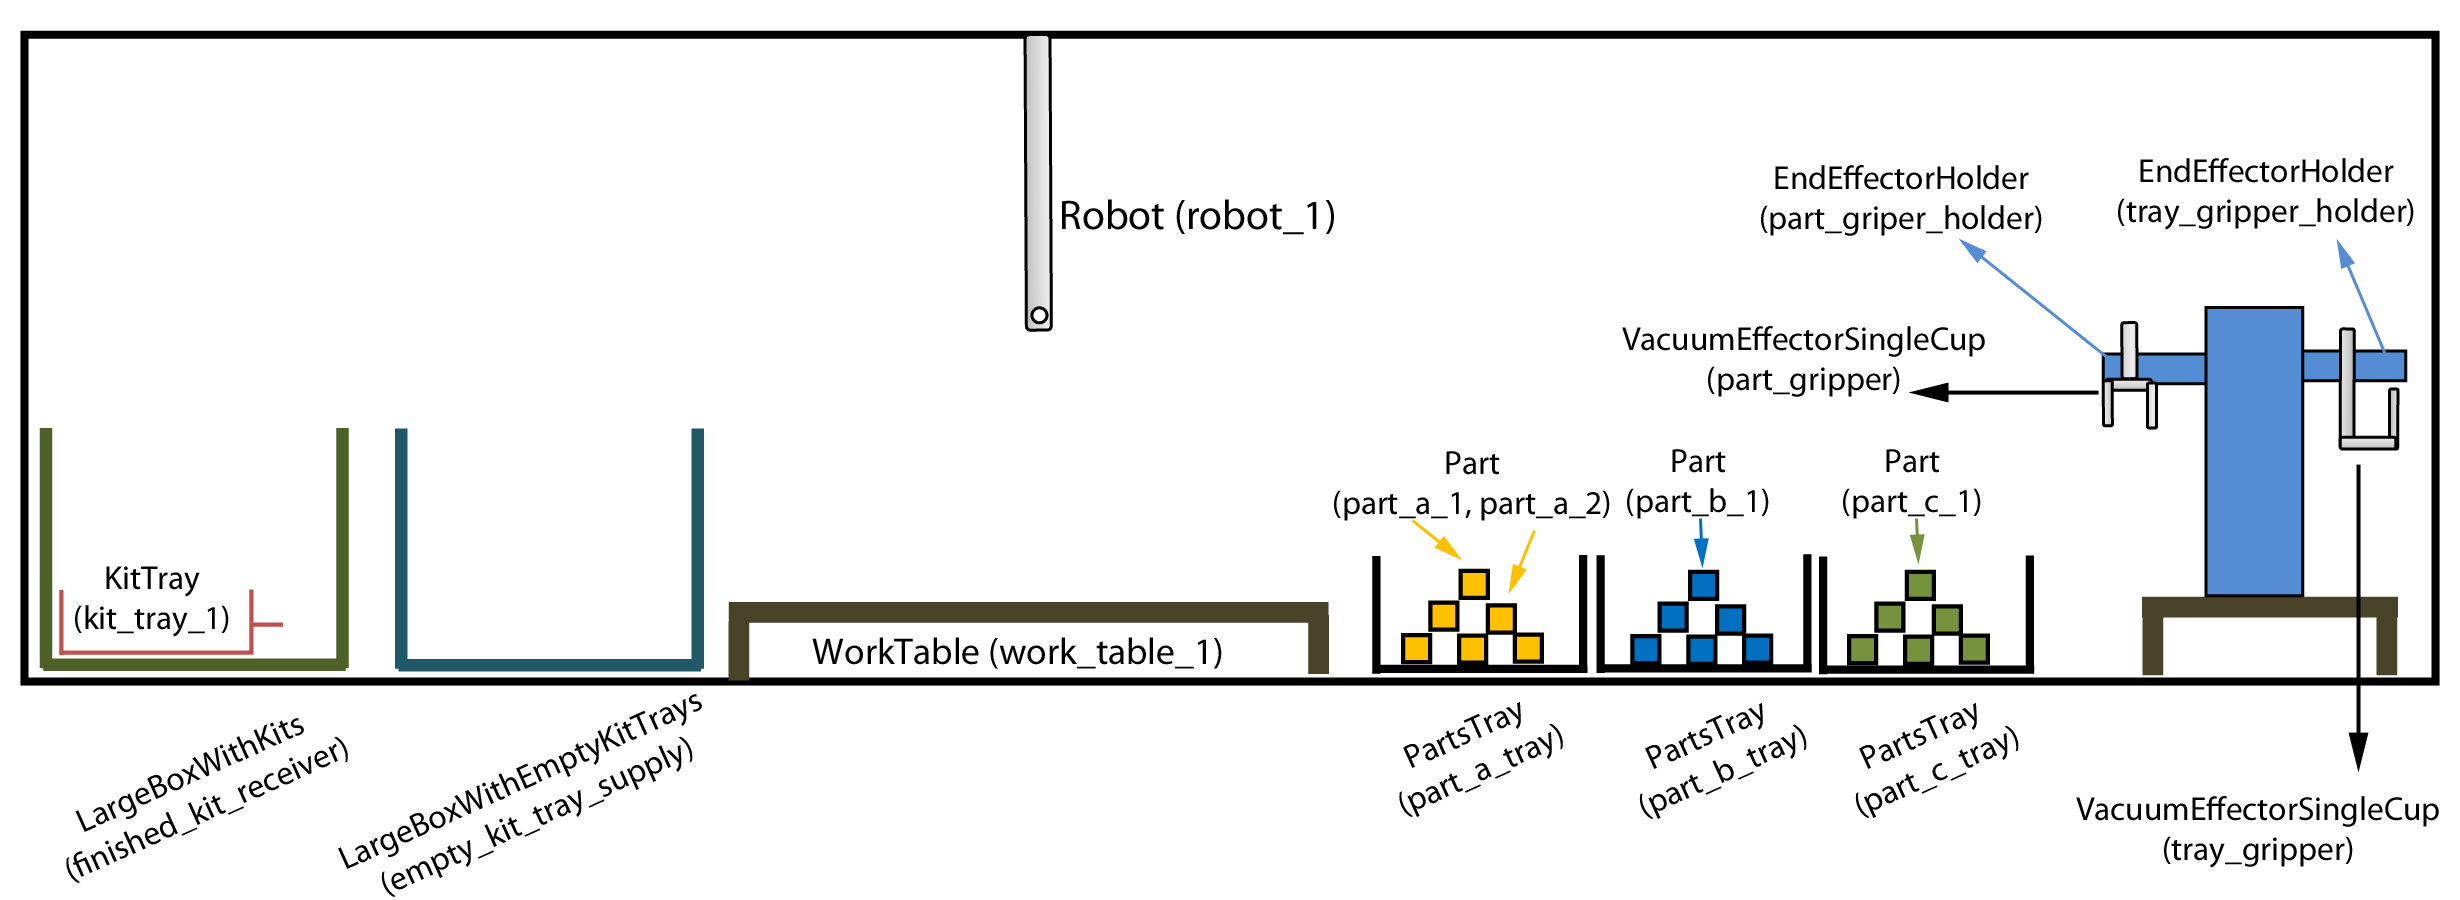
\includegraphics[width=14cm]{Figure/s0.jpg}
\caption{Initial state $S_0$.}
\label{fig:s0}
\end{figure}

\begin{itemize}
\item line 19: \texttt{:init} signals a planner that the predicates and functions in this section are true in the initial state.
\item line 20--76: Predicates true in the initial state of the environment. Since PDDL uses a close world assumption, predicates that are not present in the initial state are automatically set to false. This section also set the initial values for functions. Some relevant sections are presented:
\begin{itemize}
\item line 21: The predicate \stvarsmall{part-not-searched} is set to true so that the operator \op{look-for-part} can be activated during a plan search.
\item line 58--60: Functions describing how many parts of a specific type that \constsmall{kit\_a2b1c1} can contain. In this example, \constsmall{kit\_a2b1c1} can have two \class{Parts} of type A (\constsmall{part\_a\_tray}), one \class{Part} of type B (\constsmall{part\_b\_tray}), and one \class{Part} of type C (\constsmall{part\_c\_tray}).
\item line 62--64: Functions that represent the number of parts of a specific type that are already in \constsmall{kit\_a2b1c1}. In the initial state, \constsmall{kit\_a2b1c1} is empty (no \class{Parts} of type A, B, or C).
\item line 65--67: Functions that describe the number of parts available in their respective parts tray. This also can be read as: \emph{In the workstation, there are two \class{Parts} of type A available, three \class{Parts} of type B available, and three \class{Parts} of type C available}.
\item line 69--75: Predicates that describe the type of each specific part in the workstation. Defining that \texttt{part\_a\_1} is from \texttt{part\_a\_tray} is similar to \texttt{part\_a\_tray} is of type A since a \class{PartsTray} consists of parts of the same type.
\end{itemize}
\end{itemize}

\subsubsection{Goal State}
\begin{figure}[h!t!]
\centering
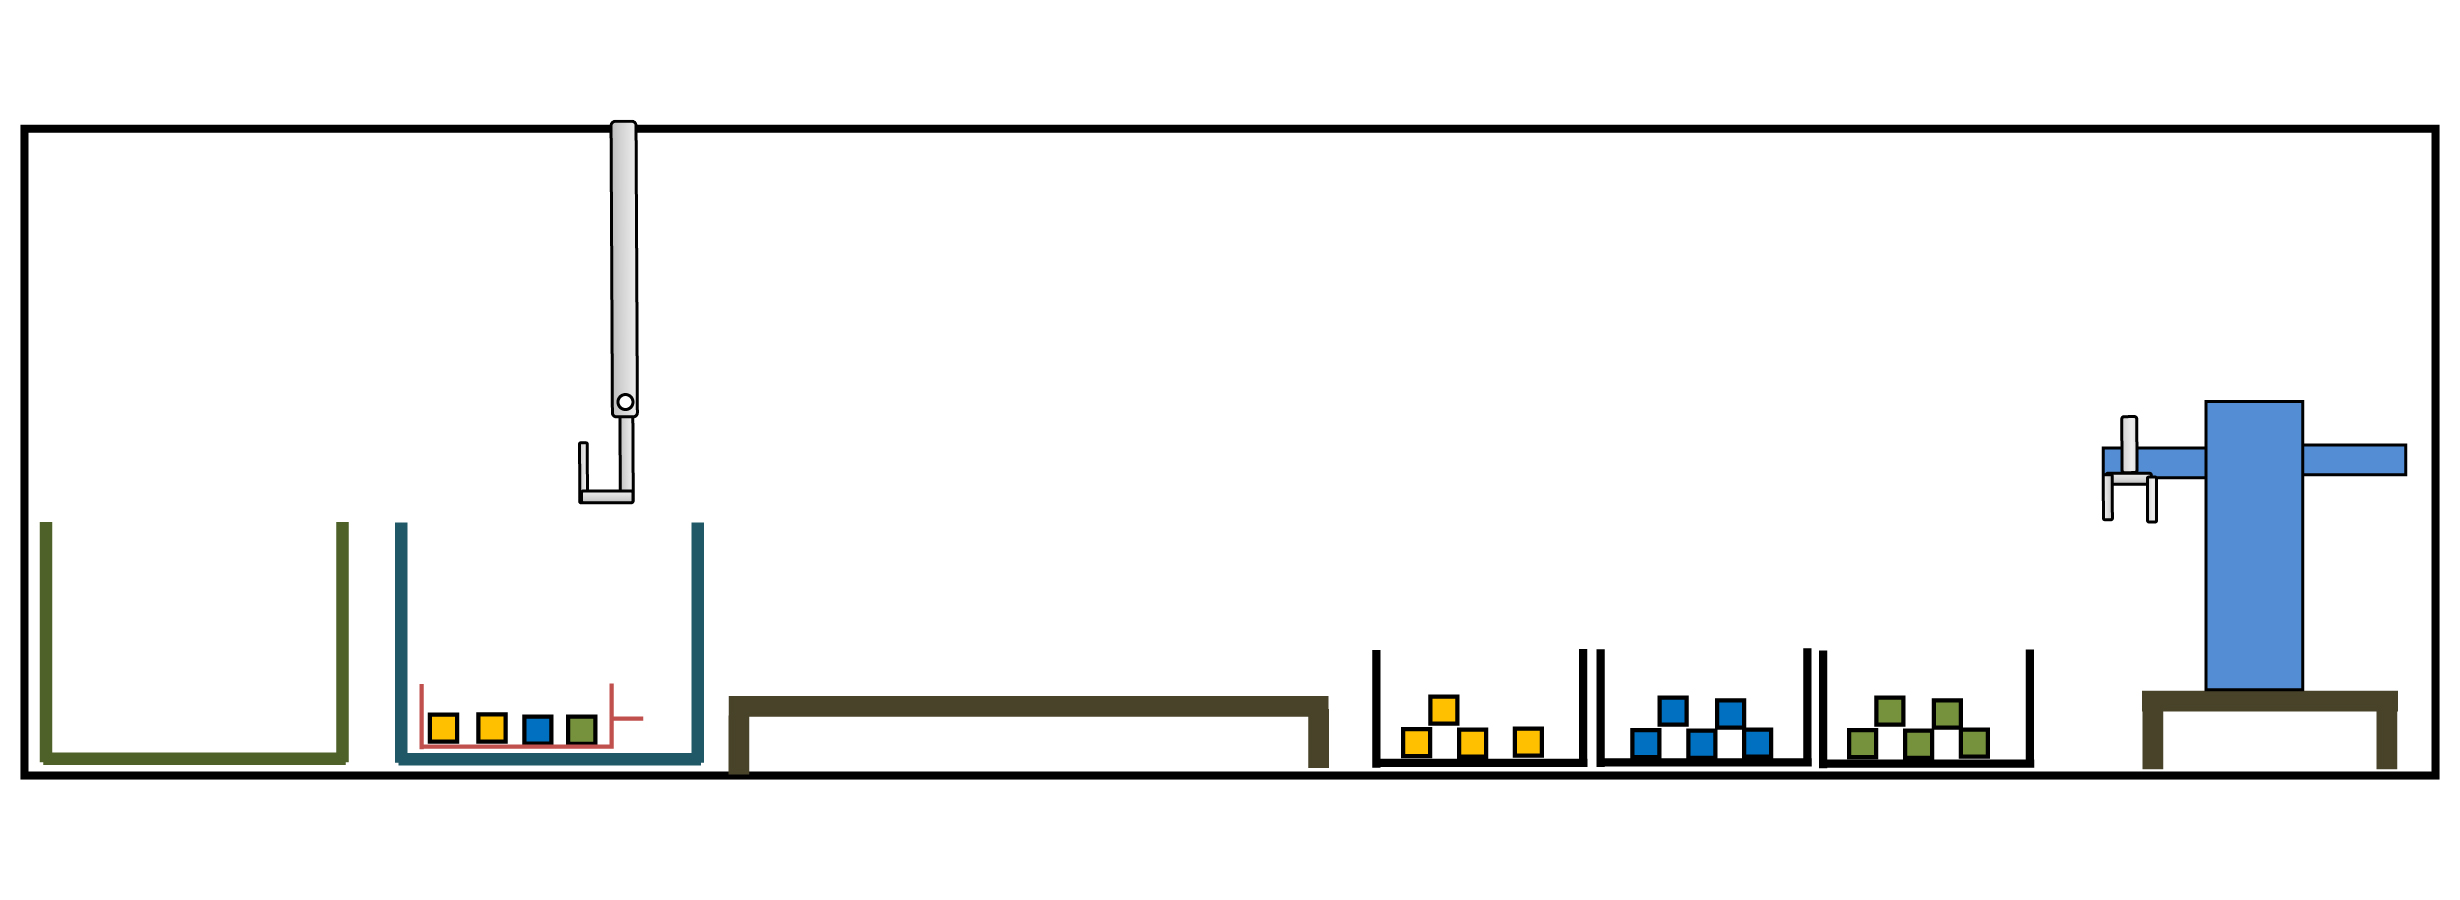
\includegraphics[width=14cm]{Figure/sfinal.jpg}
\caption{Goal state $S_G$.}
\label{fig:sf}
\end{figure}
Figure~\ref{fig:sf} depicts the goal state $S_G$ for the kitting workstation. The expression of the goal state in PDDL is described below.


\begin{itemize}
\item line 78: \texttt{:goal} is a keyword used to signal a planner about the goal state to reach. All the predicates and functions in the goal state must be true.
\item line 80--82: The quantity of parts of a specific type in \constsmall{kit\_a2b1c1} should match the capacity of parts of a specific type for \constsmall{kit\_a2b1c1}. The quantity of parts in \constsmall{kit\_a2b1c1} is increased in the operator \op{put-part}. The initial quantity of parts in \constsmall{kit\_a2b1c1} (lines 62--64) and its capacity (lines 58--60) are set in the initial state. Note that we are not specifying which instance of \class{Part} should go in \constsmall{kit\_a2b1c1} but rather the number of \class{Parts} of a specific type that \constsmall{kit\_a2b1c1} must have.
\item line 83: \constsmall{kit\_a2b1c1} should be placed in the large box with kits \constsmall{finished\_kit\_receiver}.
\end{itemize}

\subsection{Plan}
This section shows an example of a plan generated by a planner (see section~\ref{section:planner}) for the PDDL domain and problem files discussed previously in this document.

 Figure~\ref{fig:plan} displays the different states and actions used by the planner to generate a plan starting from the initial state $S_0$ to the goal state $S_G$. The actions $A_1$ \ldots $A_{17}$ are described below.
\begin{itemize}
\item $A1$:(\opsmall{attach-endeffector} \constsmall{robot\_1} \constsmall{tray\_gripper} \constsmall{tray\_gripper\_holder} \constsmall{changing\_station\_1})
\item $A2$:(\opsmall{take-kittray} \constsmall{robot\_1} \constsmall{kit\_tray\_1} \constsmall{empty\_kit\_tray\_supply} \constsmall{tray\_gripper} \constsmall{work\_table\_1})
\item $A3$:(\opsmall{put-kittray} \constsmall{robot\_1} \constsmall{kit\_tray\_1} \constsmall{work\_table\_1})
\item $A4$:(\opsmall{create-kit} \constsmall{kit\_a2b2c1} \constsmall{kit\_tray\_1} \constsmall{work\_table\_1})
\item $A5$:(\opsmall{remove-endeffector} \constsmall{robot\_1} \constsmall{tray\_gripper} \constsmall{tray\_gripper\_holder} \constsmall{changing\_station\_1})
\item $A6$:(\opsmall{attach-endeffector} \constsmall{robot\_1} \constsmall{part\_gripper} \constsmall{part\_gripper\_holder} \constsmall{changing\_station\_1})
\item $A7$:(\opsmall{look-for-part} \constsmall{robot\_1} \constsmall{part\_c\_1} \constsmall{part\_c\_tray} \constsmall{kit\_a2b2c1} \constsmall{work\_table\_1} \constsmall{part\_gripper})
\item $A8$:(\opsmall{take-part} \constsmall{robot\_1} \constsmall{part\_c\_1} \constsmall{part\_c\_tray} \constsmall{part\_gripper} \constsmall{work\_table\_1} \constsmall{kit\_a2b2c1})
\item $A9$:(\opsmall{put-part} \constsmall{robot\_1} \constsmall{part\_c\_1} \constsmall{kit\_a2b2c1} \constsmall{work\_table\_1} \constsmall{part\_c\_tray})
\item $A10$:(\opsmall{look-for-part} \constsmall{robot\_1} \constsmall{part\_b\_2} \constsmall{part\_b\_tray} \constsmall{kit\_a2b2c1} \constsmall{work\_table\_1} \constsmall{part\_gripper})
\item $A11$:(\opsmall{take-part} \constsmall{robot\_1} \constsmall{part\_b\_2} \constsmall{part\_b\_tray} \constsmall{part\_gripper} \constsmall{work\_table\_1} \constsmall{kit\_a2b2c1})
\item $A12$:(\opsmall{put-part} \constsmall{robot\_1} \constsmall{part\_b\_2} \constsmall{kit\_a2b2c1} \constsmall{work\_table\_1} \constsmall{part\_b\_tray})
\item $A13$:(\opsmall{look-for-part} \constsmall{robot\_1} \constsmall{part\_b\_1} \constsmall{part\_b\_tray} \constsmall{kit\_a2b2c1} \constsmall{work\_table\_1} \constsmall{part\_gripper})
\item $A14$:(\opsmall{take-part} \constsmall{robot\_1} \constsmall{part\_b\_1} \constsmall{part\_b\_tray} \constsmall{part\_gripper} \constsmall{work\_table\_1} \constsmall{kit\_a2b2c1})
\item $A15$:(\opsmall{put-part} \constsmall{robot\_1} \constsmall{part\_b\_1} \constsmall{kit\_a2b2c1} \constsmall{work\_table\_1} \constsmall{part\_b\_tray})
\item $A16$:(\opsmall{look-for-part} \constsmall{robot\_1} \constsmall{part\_a\_2} \constsmall{part\_a\_tray} \constsmall{kit\_a2b2c1} \constsmall{work\_table\_1} \constsmall{part\_gripper})
\item $A17$:(\opsmall{take-part} \constsmall{robot\_1} \constsmall{part\_a\_2} \constsmall{part\_a\_tray} \constsmall{part\_gripper} \constsmall{work\_table\_1} \constsmall{kit\_a2b2c1})
\item $A18$:(\opsmall{put-part} \constsmall{robot\_1} \constsmall{part\_a\_2} \constsmall{kit\_a2b2c1} \constsmall{work\_table\_1} \constsmall{part\_a\_tray})
\item $A19$:(\opsmall{look-for-part} \constsmall{robot\_1} \constsmall{part\_a\_1} \constsmall{part\_a\_tray} \constsmall{kit\_a2b2c1} \constsmall{work\_table\_1} \constsmall{part\_gripper})
\item $A20$:(\opsmall{take-part} \constsmall{robot\_1} \constsmall{part\_a\_1} \constsmall{part\_a\_tray} \constsmall{part\_gripper} \constsmall{work\_table\_1} \constsmall{kit\_a2b2c1})
\item $A21$:(\opsmall{put-part} \constsmall{robot\_1} \constsmall{part\_a\_1} \constsmall{kit\_a2b2c1} \constsmall{work\_table\_1} \constsmall{part\_a\_tray})
\item $A22$:(\opsmall{remove-endeffector} \constsmall{robot\_1} \constsmall{part\_gripper} \constsmall{part\_gripper\_holder} \constsmall{changing\_station\_1})
\item $A23$:(\opsmall{attach-endeffector} \constsmall{robot\_1} \constsmall{tray\_gripper} \constsmall{tray\_gripper\_holder} \constsmall{changing\_station\_1})
\item $A24$:(\opsmall{take-kit} \constsmall{robot\_1} \constsmall{kit\_a2b2c1} \constsmall{work\_table\_1} \constsmall{tray\_gripper})
\item $A25$:(\opsmall{put-kit} \constsmall{robot\_1} \constsmall{kit\_a2b2c1} \constsmall{finished\_kit\_receiver})
\end{itemize}

\begin{figure}[h!]
\centering
%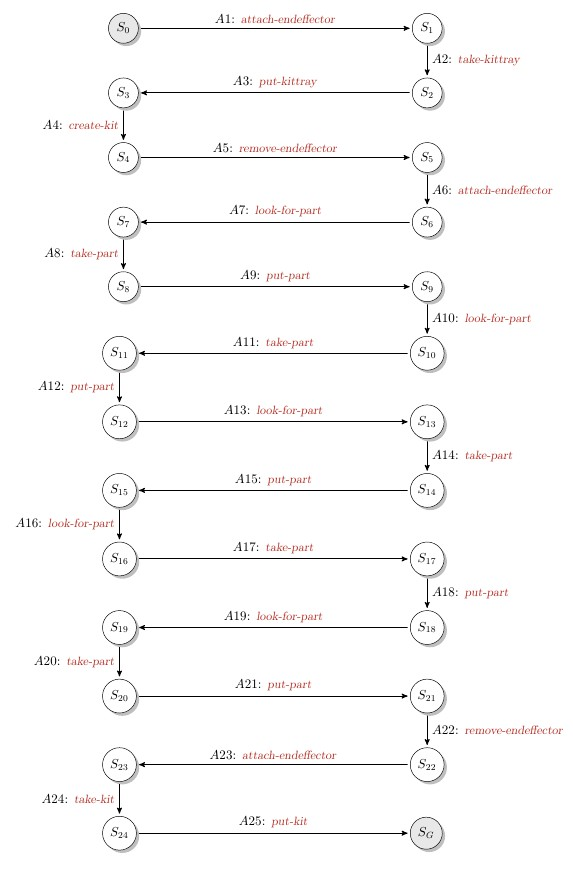
\includegraphics[width=12cm]{Figure/generated-plan.jpg}
\scalebox{.7}{
\begin{tikzpicture}[node distance=1.5cm, every edge/.style={link}]

  %%%%%%%%%%%%%%%%%%%%%%%%%%%%%%%%%%%%%%%%%%%%
  %---------- Main
  %%%%%%%%%%%%%%%%%%%%%%%%%%%%%%%%%%%%%%%%%%%%
  \node[cloud2] (S0)  {$S_0$};
  \node[cloud] (S1) [right=8cm of S0]{$S_1$};
  \node[cloud] (S2) [below=1cm of S1]{$S_2$};
  \node[cloud] (S3) [left=8cm of S2]{$S_3$};
  \node[cloud] (S4) [below=1cm of S3]{$S_4$};
  \node[cloud] (S5) [right=8cm of S4]{$S_5$};
  \node[cloud] (S6) [below=1cm of S5]{$S_6$};
  \node[cloud] (S7) [left=8cm of S6]{$S_7$};
  \node[cloud] (S8) [below=1cm of S7]{$S_8$};
  \node[cloud] (S9) [right=8cm of S8]{$S_9$};
  \node[cloud] (S10) [below=1cm of S9]{$S_{10}$};
  \node[cloud] (S11) [left=8cm of S10]{$S_{11}$};
  \node[cloud] (S12) [below=1cm of S11]{$S_{12}$};
  \node[cloud] (S13) [right=8cm of S12]{$S_{13}$};
  \node[cloud] (S14) [below=1cm of S13]{$S_{14}$};
  \node[cloud] (S15) [left=8cm of S14]{$S_{15}$};
  \node[cloud] (S16) [below=1cm of S15]{$S_{16}$};
  \node[cloud] (S17) [right=8cm of S16]{$S_{17}$};
  \node[cloud] (S18) [below=1cm of S17]{$S_{18}$};
  \node[cloud] (S19) [left=8cm of S18]{$S_{19}$};
  \node[cloud] (S20) [below=1cm of S19]{$S_{20}$};
  \node[cloud] (S21) [right=8cm of S20]{$S_{21}$};
  \node[cloud] (S22) [below=1cm of S21]{$S_{22}$};
  \node[cloud] (S23) [left=8cm of S22]{$S_{23}$};
  \node[cloud] (S24) [below=1cm of S23]{$S_{24}$};
  \node[cloud2] (SG) [right=8cm of S24]{$S_G$};

\draw[myarrow] (S0.east) -- node [above] {$A1$: \opsmall{attach-endeffector}}(S1.west);
\draw[myarrow] (S1.south) -- node [right] {$A2$: \opsmall{take-kittray}}(S2.north);
\draw[myarrow] (S2.west) --  node [above] {$A3$: \opsmall{put-kittray}}(S3.east);
\draw[myarrow] (S3.south) --  node [left] {$A4$: \opsmall{create-kit}}(S4.north);
\draw[myarrow] (S4.east) --  node [above] {$A5$: \opsmall{remove-endeffector}}(S5.west);
\draw[myarrow] (S5.south) --  node [right] {$A6$: \opsmall{attach-endeffector}}(S6.north);
\draw[myarrow] (S6.west) --  node [above] {$A7$: \opsmall{look-for-part}}(S7.east);
\draw[myarrow] (S7.south) --  node [left] {$A8$: \opsmall{take-part}}(S8.north);
\draw[myarrow] (S8.east) --  node [above] {$A9$: \opsmall{put-part}}(S9.west);
\draw[myarrow] (S9.south) --  node [right] {$A10$: \opsmall{look-for-part}}(S10.north);
\draw[myarrow] (S10.west) --  node [above] {$A11$: \opsmall{take-part}}(S11.east);
\draw[myarrow] (S11.south) --  node [left] {$A12$: \opsmall{put-part}}(S12.north);
\draw[myarrow] (S12.east) --  node [above] {$A13$: \opsmall{look-for-part}}(S13.west);
\draw[myarrow] (S13.south) --  node [right] {$A14$: \opsmall{take-part}}(S14.north);
\draw[myarrow] (S14.west) --  node [above] {$A15$: \opsmall{put-part}}(S15.east);
\draw[myarrow] (S15.south) -- node [left] {$A16$: \opsmall{look-for-part}}(S16.north);
\draw[myarrow] (S16.east) -- node [above] {$A17$: \opsmall{take-part}}(S17.west);
\draw[myarrow] (S17.south) -- node [right] {$A18$: \opsmall{put-part}}(S18.north);
\draw[myarrow] (S18.west) -- node [above] {$A19$: \opsmall{look-for-part}}(S19.east);
\draw[myarrow] (S19.south) -- node [left] {$A20$: \opsmall{take-part}}(S20.north);
\draw[myarrow] (S20.east) -- node [above] {$A21$: \opsmall{put-part}}(S21.west);
\draw[myarrow] (S21.south) -- node [right] {$A22$: \opsmall{remove-endeffector}}(S22.north);
\draw[myarrow] (S22.west) -- node [above] {$A23$: \opsmall{attach-endeffector}}(S23.east);
\draw[myarrow] (S23.south) -- node [left] {$A24$: \opsmall{take-kit}}(S24.north);
\draw[myarrow] (S24.east) -- node [above] {$A25$: \opsmall{put-kit}}(SG.west);

\end{tikzpicture}
}
\caption{Example of plan generated with the kitting domain and problem files.}
\label{fig:plan}
\end{figure} 
\section{Robot Language}
%\section{State-Variable Representation}
In a SVR, each state is represented by a tuple of values of $n$ state variables $\lbrace x_1,\dots,x_n\rbrace$, and each action is represented by a partial function that maps this tuple into some other tuple of values of the $n$ state variables.\\ \\
To build the SVR, the group has taken a very systematic approach of identifying and modeling the concepts. Because the industrial robot field is so broad, the group decided to limit its efforts to a single type of operation, namely kitting. A scenario was developed that described, in detail, the types of operations that would be performed in kitting, the sequencing of steps, the parts and machines that were needed, constraints on the process such as pre- and post-conditions, etc. For this scenario, a set of concepts were extracted and defined. These concepts served as the initial requirements for the kitting SVR. The concepts were then modeling in our SVR, building off of the definitions and relationships that were identified in the scenario. A SVR relies on the elements of constant variable symbols, object variable symbols, state variable symbols, rigid relations, and planning operators. These are defined for the kitting domain in the rest of this section.


\subsection{Constant Variable Symbols}
For the kitting domain, there is a finite set of constant variable symbols that must be represented. In the SVR, constant variable symbols are partitioned into disjoint classes corresponding to the objects of the domain. The finite set of all constant variable symbols in the kitting domain is partitioned into the following sets:
%\begin{small}
\begin{itemize}
\item A set of \class{Parts} \{\const{part_1},\const{part_2},\ldots\}: \class{Parts} are the basic items that will be used to fill a kit.

\item A set of \class{PartTrays} \{\const{pt_1},\const{pt_2},\ldots\}: \class{Parts} arrive at the workstation in \class{PartTrays}. Each part is at a known position in the \class{PartTray}. Each \class{PartTray} contains one type of \class{Part}.

\item A set of \class{KitTrays} \{\const{kt_1},\const{kt_2},\ldots\}:  A \class{KitTray} can hold \class{Parts} in known positions.

\item A set of \class{KitInstances} \{\const{kins_1},\const{kins_2},\ldots\}: A \class{KitInstance} consists of a \class{KitTray} and, possibly, some \class{Parts}. A \class{KitInstance} is empty when it does not contain any \class{Part} and finished when it contains all the \class{Parts} that constitute a kit.

\item A symbol \class{WorkTable} -- \const{wtable}: A \class{WorkTable} is an area in the kitting workstation where \class{KitTrays} are placed to build \class{KitInstances}.

\item A set of \class{LargeBoxWithKits} \{\const{lbwk_1},\const{lbwk_2},\ldots\}: A \class{LargeBoxWithKits} contains only finished \class{KitInstances}.

\item A set of \class{LargeBoxWithEmptyKitTrays} \{\const{lbwekt_1}, \const{lbwekt_2},\ldots\}: A \class{LargeBoxWithEmptyKitTrays} is a box that contains only empty \class{KitTrays}.

\item A set of \class{Robots} \{\const{r_1},\const{r_2},\ldots\}: A \class{Robot} in the kitting workstation is a robotic arm that can move objects in order to build \class{KitInstances}.

\item A set of \class{EndEffectors} \{\const{eff_1},\const{eff_2},\ldots\}: \class{EndEffectors} are used in a kitting workstation to manipulate \class{Parts}, \class{PartTrays}, \class{KitTrays}, and \class{KitInstances}. An \class{EndEffector} is attached to a \class{Robot}.

\item A set of \class{EndEffectorHolders}  \{\const{effh_1},\const{effh_2}, \ldots\}: An \class{EndEffectorHolder} is a storage unit that holds one type of \class{EndEffector}.

\item A symbol \class{EndEffectorChangingStation} -- \const{chstation}: An \class{EndEffectorChangingStation} is made up of \class{EndEffectorHolders}.
\end{itemize}
%\end {small}

\subsection{Object Variable Symbols}
Object variable symbols are typed variables which range over a class or the union of classes of constant variable symbols. Examples of object variable symbols are \const{r} $\in$ \class{Robots}, \const{kt} $\in$ \class{KitTrays}, etc.

\subsection{State Variable Symbols}
\label{subsubsect:State_Variable_Symbols}
A state variable symbol is defined as follows:
$\mathrm{x: A_1\times \dots\times A_i\times S\rightarrow B_1\cup\dots\cup B_j}$ ($i, j\geq 1$) is a function from the set of states ($\mathrm{S}$) and at least one set of constant variable symbols $\mathrm{A_1\times \dots\times A_i}$ into a set of constant variable symbols $\mathrm{B_1\cup\dots\cup B_j}$.\\

\noindent
The use of state variable symbols reduces the possibility of inconsistent states and generates a smaller state space. The following state variable symbols are used in the kitting domain:

\begin{itemize}
\item \stvar{efflocation}: \class{EndEffectors}$\mathrm{\times S\rightarrow}$\class{Robots} $\cup$ \class{EndEffectorHolders}: designates the location of an \class{EndEffector} in the workstation, i.e., in a \class{EndEffectorHolder} or attached to a \class{Robot}.

\item \stvar{r-eff}: \class{Robots}$\mathrm{\times S\rightarrow}$\class{EndEffectors} $\cup$ \{\textit{nil}\}: designates the \class{EndEffector} attached to a \class{Robot} if there is one attached, otherwise \textit{nil}.

\item \stvar{on-worktable}: \class{WorkTable}$\mathrm{\times S\rightarrow}$\class{KitInstances} $\cup$ \class{KitTrays} $\cup$ \{\textit{nil}\}: designates the object placed on the \class{WorkTable}, i.e., a \class{KitInstance}, a \class{KitTray}, or nothing (\textit{nil}).

\item \stvar{kinslocation}: \class{KitInstances}$\mathrm{\times S\rightarrow}$\class{LargeBoxWithKits} $\cup$ \class{WorkTable} $\cup$ \class{Robots}: designates the different possible locations of a \class{KitInstance} in the workstation, i.e., in a \class{LargeBoxWithKits}, on the \class{WorkTable}, or being held by a \class{Robot}.

\item \stvar{ktlocation}: \class{KitTrays}$\mathrm{\times S\rightarrow}$\class{LargeBoxWithEmptyKitTrays} $\cup$ \class{Robots} $\cup$ \class{WorkTable}: designates the different possible locations of a \class{KitTray} in the workstation, i.e., in a \class{LargeBoxWithEmptyKitTrays}, on a \class{WorkTable} or being held by a \class{Robot}.

\item \stvar{partlocation}: \class{Parts}$\mathrm{\times S\rightarrow}$\class{PartTrays} $\cup$ \class{KitInstances} $\cup$ \class{Robots}: designates the different possible locations of a \class{Part} in the workstation, i.e., in a \class{PartTray}, in a \class{KitInstance}, or being held by a \class{Robot}.

\item \stvar{rhold}: \class{Robots}$\mathrm{\times S\rightarrow}$\class{KitTrays} $\cup$ \class{KitInstances} $\cup$ \class{Parts} $\cup$ \{\textit{nil}\}: designates the object being held by a \class{Robot}, i.e., a \class{KitTray}, a \class{KitInstance}, \class{Part}, or nothing (\textit{nil}). It is assumed that the \class{Robot} is already equipped with the appropriate \class{EndEffector}.

\item \stvar{islbwkfull}: \class{LargeBoxWithKits}$\mathrm{\times S\rightarrow}$ \{0\} $\cup$ \{1\}: designates if a \class{LargeBoxWithKits} is full (1) or not (0).

\item \stvar{islbwektempty}: \class{LargeBoxWithEmptyKitTrays}$\mathrm{\times S\rightarrow}$ \{0\} $\cup$ \{1\}: designates if a \class{LargeBoxWithEmptyKitTrays} is empty (1) or not (0).

\item \stvar{isptempty}: \class{PartTrays}$\mathrm{\times S\rightarrow}$ \{0\} $\cup$ \{1\}: designates if a \class{PartTray} is empty (1) or not (0).

\item \stvar{efftype}: \class{EndEffectors}$\mathrm{\times S \rightarrow}$\class{KitTrays} $\cup$ \class{KitInstances} $\cup$ \class{Parts}: designates the type of object an \class{EndEffector} can hold, i.e., \class{KitTrays}, \class{KitInstances}, or \class{Parts}.

\item \stvar{effhold-eff}: \class{EndEffectorHolders}$\mathrm{\times S \rightarrow}$\class{EndEffectors}: designates the \class{EndEffector} that an \class{EndEffectorHolder} can hold.
\end{itemize}


\subsection{Rigid Relations}
\label{subsubsect:Rigid_Relation}
\stvar{efftype} and \stvar{effhold-eff} are rigid relations since their values do not vary from one state to another. In each state, a given \class{EndEffector} will always hold the same type of object and a given \class{EndEffectorHolder} will always hold the same \class{EndEffectors}.

\subsection{Planning Operators and Actions}
\label{subsect:Planning_Operators}
The planning operators presented in this section will be expressed in classical representation instead of state variable representation. In classical representation, states are represented as sets of logical atoms that are true or false within some interpretation. Actions are represented by planning operators that change the truth values of these atoms. Predicates and actions in the domain and problem PDDL files (see Section~\ref{S:PDDL}) need to be expressed with logical atoms, hence the use of classical representation.

\subsubsection{Convert State Variable Symbols to Atoms}
In order to use sets of logical atoms, the state variable symbols presented in Section~\ref{subsubsect:State_Variable_Symbols} are converted into predicates (PRED).

In the rest of this section, the state variable symbols (SVSs) and their corresponding predicates (PREDs) are presented as follows:
\begin{itemize}
 \item \stvar{SVS}
  \begin{itemize}
  \item \stvar{PRED1} (\class{param1},\class{param2}, \ldots)
  \item \stvar{PRED2} (\class{param1},\class{param2}, \ldots)
  \end{itemize}
\end{itemize}


The SVSs and PREDs for kitting are presented below:
\begin{itemize}
 \item \stvar{efflocation}
  \begin{itemize}
  \item \stvar{efflocation}(\class{EndEffector},\class{Robot}) ;TRUE iff EndEffector is attached to Robot
  \item \stvar{efflocation}(\class{EndEffector},\class{EndEffectorHolder}) ;TRUE iff EndEffector is in EndEffectorHolder
  \end{itemize}

 \item \stvar{r-eff}
  \begin{itemize}
  \item \stvar{r-with-eff}(\class{Robot},\class{EndEffector}) ;TRUE iff \class{Robot} is equipped with \class{EndEffector}
  \item \stvar{r-no-eff}(\class{Robot}) ;TRUE iff \class{Robot} is not equipped with any \class{EndEffector}	
  \end{itemize}

 \item \stvar{on-worktable}
  \begin{itemize}
  \item \stvar{onworktable}(\class{WorkTable},\class{KitInstance}) ;TRUE iff \class{KitInstance} is on \class{WorkTable}
  \item \stvar{onworktable}(\class{WorkTable},\class{KitTray}) ;TRUE iff \class{KitTray} is on \class{WorkTable}
  \item \stvar{worktable-empty}(\class{WorkTable}) ;TRUE iff there is nothing on \class{WorkTable}
  \end{itemize}

 \item \stvar{kinslocation}
  \begin{itemize}
  \item \stvar{kinslocation}(\class{KitInstance},\class{LargeBoxWithKit}) ;TRUE iff \class{KitInstance} is in \class{LargeBoxWithKit}
  \item \stvar{kinslocation}(\class{KitInstance},\class{WorkTable}) ;TRUE iff \class{KitInstance} is on \class{WorkTable}
  \item \stvar{kinslocation}(\class{KitInstance},\class{Robot}) ;TRUE iff \class{KitInstance} is being held by \class{Robot}	
  \end{itemize}

 \item \stvar{ktlocation}
  \begin{itemize}
  \item \stvar{ktlocation}(\class{KitTray},\class{LargeBoxWithEmptyKitTray}) ;TRUE iff \class{KitTray} is in \class{LargeBoxWithEmptyKitTray}	
  \item \stvar{ktlocation}(\class{KitTray},\class{Robot}) ;TRUE iff \class{KitTray} is being held by \class{Robot}
  \item \stvar{ktlocation}(\class{KitTray},\class{WorkTable}) ;TRUE iff \class{KitTray} is on \class{WorkTable}
  \end{itemize}

 \item \stvar{partlocation}
  \begin{itemize}
    \item \stvar{partlocation}(\class{Part},\class{PartTray}) ;TRUE iff \class{Part} is in \class{PartTray}	
    \item \stvar{partlocation}(\class{Part},\class{KitInstance}) ;TRUE iff \class{Part} is in \class{KitInstance}
    \item \stvar{partlocation}(\class{Part},\class{Robot}) ;TRUE iff \class{Part} is being held by \class{Robot}
  \end{itemize}

 \item \stvar{rhold}
  \begin{itemize}
    \item \stvar{rhold}(\class{Robot},\class{KitTray}) ;TRUE iff \class{Robot} is holding \class{KitTray}	
    \item \stvar{rhold}(\class{Robot},\class{KitInstance}) ;TRUE iff \class{Robot} is holding \class{KitInstance}
    \item \stvar{rhold}(\class{Robot},\class{Part}) ;TRUE iff \class{Robot} is holding \class{Part}
    \item \stvar{rhold-empty}(\class{Robot}) ;TRUE iff \class{Robot} is not holding anything
  \end{itemize}

 \item \stvar{islbwkfull}
  \begin{itemize}
    \item \stvar{lbwk-non-full}(\class{LargeBoxWithKit}) ;TRUE iff \class{LargeBoxWithKit} is not full	 
  \end{itemize}

 \item \stvar{islbwektempty}
  \begin{itemize}
    \item \stvar{lbwekt-non-empty}(\class{LargeBoxWithEmptyKitTray}) ;TRUE iff \class{LargeBoxWithEmptyKitTray} is not empty
  \end{itemize}

 \item \stvar{isptempty}
  \begin{itemize}
    \item \stvar{part-tray-non-empty}(\class{PartTray}) ;TRUE iff \class{PartTray} is not empty
  \end{itemize}

 \item \stvar{efftype}
  \begin{itemize}
    \item \stvar{efftype}(\class{EndEffector},\class{KitTray}) ;TRUE iff \class{EndEffector} is designed to handle \class{KitTray}	
    \item \stvar{efftype}(\class{EndEffector},\class{KitInstance}) ;TRUE iff \class{EndEffector} is designed to handle \class{KitInstance}
    \item \stvar{efftype}(\class{EndEffector},\class{Part}) ;TRUE iff \class{EndEffector} is designed to handle \class{Part}
  \end{itemize}

 \item \stvar{effhold-eff}
  \begin{itemize}
    \item \stvar{effhold-eff}(\class{EndEffectorHolder},\class{EndEffector}) ;TRUE iff \class{EndEffectorHolder} is holding \class{EndEffector}
  \end{itemize}
\end{itemize}


\subsubsection{Planning Operators}
 In classical planning, a planning operator~\cite{NAU.2004} is a triple \textit{o=(name(o), precond(o), effects(o))} whose elements are as follows:
\begin{itemize}
\item name(o) is a syntactic expression of the form $n(x_1,\dots,x_k)$, where $n$ is a symbol
called an operator symbol, $x_1,\dots,x_k$ are all of the object variable symbols that
appear anywhere in \textit{o}, and $n$ is unique (i.e., no two operators can have the
same operator symbol).
\item precond(o) and effects(o) are sets of literals (i.e., atoms and negations of atoms). Literals that are true in precond(o) but false in effects(o) are removed by using negations of the appropriate atoms.
\end{itemize}

Our kitting domain is composed of nine operators which are defined below.


\begin{enumerate}
\item \op{take-kt}(\const{r},\const{kt},\const{lbwekt},\const{eff},\const{wtable}): The \class{Robot} \const{r} equipped with the \class{EndEffector} \const{eeff} picks up the \class{KitTray} \const{kt} from the \class{LargeBoxWithEmptyKitTrays} \const{lbwekt}.

\begin{center}
\begin{tabular}{ l|l }
  \textit{precond} & \textit{effects} \\
  \hline
  \stvar{rhold-empty}(\const{r}),&$\neg$\stvar{rhold-empty}(\const{r}),\\
  \stvar{lbwekt-non-empty}(\const{lbwekt}),&\stvar{ktlocation}(\const{kt},\const{r}),\\
  \stvar{r-with-eff}(\const{r},\const{eff}),&\stvar{rhold}(\const{r},\const{kt}), \\
  \stvar{ktlocation}(\const{kt},\const{lbwekt}),&$\neg$\stvar{ktlocation}(\const{kt},\const{lbwekt}) \\
  \stvar{efflocation}(\const{eff},\const{r}),&\\
  \stvar{worktable-empty}(\const{wtable}),& \\
  \stvar{efftype}(\const{eff},\const{kt})&
\end{tabular}
\end{center}
%%%%%%%%%%%%%%%%%%%%%%%%%%%%%%%%%%%%%

\item \op{put-kt}(\const{r},\const{kt},\const{wtable}): The \class{Robot} \const{r} puts down the \class{KitTray} \const{kt} on the \class{WorkTable} \const{wtable}.
\begin{center}
\begin{tabular}{ l|l }
  \textit{precond} & \textit{effects} \\
  \hline
  \stvar{ktlocation}(\const{kt},\const{r}),&$\neg$\stvar{ktlocation}(\const{kt},\const{r}),\\
  \stvar{rhold}(\const{r},\const{kt}),&$\neg$\stvar{rhold}(\const{r},\const{kt}),\\
  \stvar{worktable-empty}(\const{wtable})&$\neg$\stvar{worktable-empty}(\const{wtable}),\\
  &\stvar{ktlocation}(\const{kt},\const{wtable}),\\
  &\stvar{rhold-empty}(\const{r}),\\
  &\stvar{onworktable}(\const{wtable},\const{kt})\\
\end{tabular}
\end{center}
%%%%%%%%%%%%%%%%%%%%%%%%%%%%%%%%%%%%%

\item \op{take-kins}(\const{r},\const{kins},\const{wtable},\const{eff}): The \class{Robot} \const{r} equipped with the \class{EndEffector} \const{eff} picks up the \class{KitInstance} \const{kins} from the \class{WorkTable} \const{wtable}.
\begin{center}
\begin{tabular}{ l|l }
  \textit{precond} & \textit{effects} \\
  \hline
  \stvar{kinslocation}(\const{kins},\const{wtable}),&$\neg$\stvar{kinslocation}(\const{kins},\const{wtable}),\\
  \stvar{rhold-empty}(\const{r}),&$\neg$\stvar{rhold-empty}(\const{r}),\\
  \stvar{onworktable}(\const{wtable},\const{kins}),&$\neg$\stvar{onworktable}(\const{wtable},\const{kins}),\\
  \stvar{r-with-eff}(\const{r},\const{eff}),&\stvar{kinslocation}(\const{kins},\const{r}),\\
  \stvar{efftype}(\const{eff},\const{kins})&\stvar{rhold}(\const{r},\const{kins}),\\
  &\stvar{worktable-empty}(\const{wtable})
\end{tabular}
\end{center}
%%%%%%%%%%%%%%%%%%%%%%%%%%%%%%%%%%%%%

\item \op{put-kins}(\const{r},\const{kins},\const{lbwk}): The \class{Robot} \const{r} puts down the \class{KitInstance} \const{kins} in the \class{LargeBoxWithKits} \const{lbwk}.
\begin{center}
\begin{tabular}{ l|l }
  \textit{precond} & \textit{effects} \\
  \hline
  \stvar{kinslocation}(\const{kins},\const{r}),&$\neg$\stvar{kinslocation}(\const{kins},\const{r}),\\
  \stvar{rhold}(\const{r},\const{kins}),&$\neg$\stvar{rhold}(\const{r},\const{kins}),\\
  \stvar{lbwk-non-full}(\const{lbwk})&\stvar{kinslocation}(\const{kins},\const{lbwk}),\\
  &\stvar{rhold-empty}(\const{r})
\end{tabular}
\end{center}
%%%%%%%%%%%%%%%%%%%%%%%%%%%%%%%%%%%%%

\item \op{take-p}(\const{r},\const{part},\const{pt},\const{eff},\const{wtable},\const{kins}): The \class{Robot} \const{r} uses the \class{EndEffector} \const{eff} to pick up the \class{Part} \const{part} from the \class{PartTray} \const{pt}.
\begin{center}
\begin{tabular}{ l|l }
  \textit{precond} & \textit{effects} \\
  \hline
  \stvar{partlocation}(\const{part},\const{pt}),&$\neg$\stvar{partlocation}(\const{part},\const{pt}),\\
  \stvar{efflocation}(\const{eff},\const{r}),&\stvar{rhold}(\const{r},\const{part}),\\
  \stvar{rhold-empty}(\const{r}),&$\neg$\stvar{rhold-empty}(\const{r}),\\
  \stvar{r-with-eff}(\const{r},\const{eff}),&\stvar{partlocation}(\const{part},\const{r})\\
  \stvar{onworktable}(\const{wtable},\const{kins}),&\\
  \stvar{kinslocation}(\const{kins},\const{wtable}),&\\
  \stvar{efftype}(\const{eff},\const{part}),&\\
  \stvar{part-tray-non-empty}(\const{pt})&
\end{tabular}
\end{center}
%%%%%%%%%%%%%%%%%%%%%%%%%%%%%%%%%%%%%

\item \op{put-p}(\const{r},\const{part},\const{kins},\const{wtable}): The \class{Robot} \const{r} puts down the \class{Part} \const{part} in the \class{KitInstance} \const{kins}.
\begin{center}
\begin{tabular}{ l|l }
  \textit{precond} & \textit{effects} \\
  \hline
  \stvar{partlocation}(\const{part},\const{r}),&$\neg$\stvar{partlocation}(\const{part},\const{r}),\\
  \stvar{rhold}(\const{r},\const{part}),&$\neg$\stvar{rhold}(\const{r},\const{part}),\\
  \stvar{onworktable}(\const{wtable},\const{kins}),&\stvar{partlocation}(\const{part},\const{kins}),\\
  \stvar{kinslocation}(\const{kins},\const{wtable})&\stvar{rhold-empty}(\const{r})
\end{tabular}
\end{center}
%%%%%%%%%%%%%%%%%%%%%%%%%%%%%%%%%%%%%

\item \op{attach-eff}(\const{r},\const{eff},\const{effh}): The \class{Robot} \const{r} attaches the \class{EndEffector} \const{eff}, situated in the \class{EndEffectorHolder} \const{effh}.
\begin{center}
\begin{tabular}{ l|l }
  \textit{precond} & \textit{effects} \\
  \hline
  \stvar{efflocation}(\const{eff},\const{effh}),&$\neg$\stvar{efflocation}(\const{eff},\const{effh}),\\
  \stvar{r-no-eff}(\const{r}),&$\neg$\stvar{r-no-eff}(\const{r}),\\
  \stvar{effhhold-eff}(\const{effh},\const{eff})&$\neg$\stvar{effhhold-eff}(\const{effh},\const{eff}),\\
  &\stvar{rhold-empty}(\const{r}),\\
  &\stvar{efflocation}(\const{eff},\const{r}),\\
  &\stvar{r-with-eff}(\const{r},\const{eff})
\end{tabular}
\end{center}
%%%%%%%%%%%%%%%%%%%%%%%%%%%%%%%%%%%%%

\item \op{remove-eff}(\const{r},\const{eff},\const{effh}): The \class{Robot} \const{r} removes the \class{EndEffector} \const{eff} and puts it in the \class{EndEffectorHolder} \const{effh}.
\begin{center}
\begin{tabular}{ l|l }
  \textit{precond} & \textit{effects} \\
  \hline
  \stvar{efflocation}(\const{eff},\const{r}),&$\neg$\stvar{efflocation}(\const{eff},\const{r}),\\
  \stvar{r-with-eff}(\const{r},\const{eff}),&$\neg$\stvar{r-with-eff}(\const{r},\const{eff}),\\
  \stvar{rhold-empty}(\const{r})&efflocation(\const{eff},\const{effh}),\\
  &\stvar{effhhold-eff}(\const{effh},\const{eff}),\\
  &\stvar{r-no-eff}(\const{r})
\end{tabular}
\end{center}
%%%%%%%%%%%%%%%%%%%%%%%%%%%%%%%%%%%%%

\item \op{create-kins}(\const{kins},\const{kt},\const{wtable}): The \class{KitTray} \const{kt} is converted to the \class{KitInstance} \const{kins} once the \class{KitTray} \const{kt} is on the \class{WorkTable} \const{wtable}.
\begin{center}
\begin{tabular}{ l|l }
  \textit{precond} & \textit{effects} \\
  \hline
  \stvar{onworktable}(\const{wtable}\const{kt})&$\neg$\stvar{onworktable}(\const{wtable},\const{kt}),\\
&\stvar{kinslocation}(\const{kins},\const{wtable}),\\
&\stvar{onworktable}(\const{wtable},\const{kins})\\
\end{tabular}
\end{center}
%%%%%%%%%%%%%%%%%%%%%%%%%%%%%%%%%%%%%
\end{enumerate}

\subsubsection{Actions}
An action \textit{a} can be obtained by substituting the object variable symbols that
appear anywhere in the operator with constant variable symbols. For instance, the operator \op{take-p}(\const{r},\const{part},\const{pt},\const{eff}) in the kitting domain can be translated into the action \op{take-p}(\const{r_1},\const{part_1},\const{pt_1},\const{eff_2}) where \const{r_1}, \const{part_1}, \const{pt_1}, and \const{eff_2} are constant variable symbols in the classes \class{Robots}, \class{Parts}, \class{PartTrays}, and \class{EndEffectors}, respectively.







%
\section{Planning Language}\label{S:PDDL}
The Planning Domain Definition Language (PDDL) \cite{PDDL} is an attempt by the domain independent planning community to formulate a standard language for planning. A community of planning researchers has been producing planning systems that comply with this formalism since the first International Planning Competition held in 1998. This competition series
continues today, with the seventh competition being held in 2011. PDDL is constantly adding extensions to the base language in order to represent more expressive problem domains. Our work is based on PDDL Version 3.\\
By placing our knowledge in a PDDL representation, we enable the use of an entire family of open source planning systems.
Each PDDL file-set consists of two files that specify the domain and the problem.

\subsection{The PDDL Domain File}\label{S:PDDL-domain}
The PDDL domain file is composed of four sections that include requirements, types, predicates and functions, and actions. An excerpt of the PDDL domain file is depicted in Figure~\ref{fig:domain}.

\begin{figure}[t!h!]
\begin{minipage}{.5\paperwidth}
\begin{mylisting}
\begin{Verbatim}[commandchars=\\\{\},fontsize=\scriptsize, numbers=left, numbersep=2pt]
(define (domain kitting-domain)
    (:requirements :strips :typing :fluents)
    (:types
        EndEffector
        EndEffectorHolder
        Kit
        KitTray
        LargeBoxWithEmptyKitTrays
        LargeBoxWithKits
        Part
        PartsTray
        EndEffectorChangingStation
        Robot
        WorkTable
    )

    (:predicates
	   (endeffector-location-robot ?endeffector - EndEffector ?robot - Robot)	
	   (on-worktable-kit ?worktable - WorkTable ?kit - Kit)
    )

    (:functions
	   (quantity-partstray ?partstray - PartsTray)
	   (quantity-kit ?kit - Kit ?partstray - PartsTray)
	   (capacity-kit ?kit - Kit ?partstray - PartsTray)
    )

    (:action take-kittray
        :parameters(
            ?robot - Robot
            ?kittray - KitTray
            ?largeboxwithemptykittrays - LargeBoxWithEmptyKitTrays
            ?endeffector - EndEffector
            ?worktable - WorkTable)
        :precondition(and
            (robot-empty ?robot)
            (lbwekt-not-empty ?largeboxwithemptykittrays)
            (robot-with-endeffector ?robot ?endeffector)
            (kittray-location-lbwekt ?kittray ?largeboxwithemptykittrays)
            (endeffector-location-robot ?endeffector ?robot)
            (worktable-empty ?worktable)
            (endeffector-type-kittray ?endeffector ?kittray))
        :effect(and
            (robot-holds-kittray ?robot ?kittray)
            (kittray-location-robot ?kittray ?robot)
            (not (robot-empty ?robot))
            (not (kittray-location-lbwekt ?kittray ?largeboxwithemptykittrays)))
    )
)

\end{Verbatim}
\end{mylisting}
\end{minipage}
\caption{Excerpt of the PDDL domain file for kitting.}
\label{fig:domain}
\end{figure}

\begin{itemize}
\item line 1: The keyword \texttt{domain} signals a planner that this file contains information on the domain. \texttt{kitting-domain} is the name given to the domain.
\item line 2: The \texttt{:requirements} field specifies which section the domain relies on. The planning system can examine this statement to determine if it is capable of solving problems in this domain. A keyword (symbol starting with a colon) used in a \texttt{:requirements} field is called a requirement flag; the domain is said to declare a requirement for that flag. The requirement flags present in the kitting domain are:
\begin{itemize}
\item \texttt{:strips}: The most basic subset of PDDL, consisting of STRIPS only.
\item \texttt{:typing}: PDDL has a special syntax for declaring parameter and object types. \texttt{:typing} allows types names in declaration of variables.
\item \texttt{:fluents}: A domain's set of requirements allow a planner to quickly tell if it is likely to be able
to handle the domain. For example, this version of the kitting world requires fluents numeric, so a straight STRIPS-representation planner would not be able to handle it. A fluent is a term (\texttt{:functions}) with time-varying value (i.e., a value that can change as a result of performing an action).
\end{itemize}
\item line 3--15:  Type names have to be declared before they are used (before \texttt{:predicates} and \texttt{:functions}). This is done with the declaration \texttt{(:types $name_1$ ... $name_n$)}.
\item line 17--20: The \texttt{:predicates} part of a domain definition specify only what are the predicate names used in the domain, and their number of arguments (and argument types, if the domain uses \texttt{:typing}). The ``meaning'' of a predicate, in the sense of for what combinations of arguments it can be true and its relationship to other predicates, is determined by the effects that actions in the domain can have on the predicate, and by what instances of the predicate are listed as true in the initial state of the problem definition.\\
    It is common to make a distinction between static and dynamic predicates. A \textit{static} predicate is not changed by any action. Thus in a problem, the true and false instances of a \textit{static} predicate will always be precisely those listed in the initial state specification of the problem definition. Note that there is no syntactic difference between \textit{static} and \textit{dynamic} predicates in PDDL, they look exactly the same in the \texttt{:predicates} declaration part of the domain.\\
    A predicate is build using the structure \texttt{(predicate\_name ?X - type\_of\_X)}. A list of parameters of the same type in a predicate can be abbreviated to \texttt{(predicate\_name ?X ?Y ?Z - type\_of\_XYZ)}. Note that the hyphen between parameter and type name is surrounded by whitespace.
\item line 22--26: A fluent is similar to a state variable/predicate except that its value is a number instead of true or false. The initial value of a function is set in the initial state of the problem file and changes when an action is executed. The declaration of functions is similar to predicates.
\item line 28--48: The domain definition contains operators (called \textit{actions} in PDDL). An action statement specifies a way that a planner affects the state of the world. The statement includes parameters, preconditions, and effects. All parts of an action definition except the name are, according to the PDDL specification, optional (although, of course, an action without effects is pretty useless). However, for an action that has no preconditions some planners may require an ``empty'' precondition, on the form :precondition () or :precondition (and), and some planners may also require an empty :parameter list for actions without parameters).
\begin{itemize}
\item line 29--34: The \texttt{:parameters} section declare all the parameters used by predicates and functions in \texttt{preconditions} and \texttt{effects}.
\item line 35--42:  The \texttt{:preconditions} section is a conjunction of predicates and functions that need to be true in the world in order for the action to be invoked.
\item line 43--47: The \texttt{:effects} equation dictates the changes in the world that will occur due to the execution of the action.
\end{itemize}
\end{itemize}


\subsection{PDDL Problem File}\label{S:PDDL-problem}
The second file of the PDDL file-set is a  problem file. The problem file specifies information about the specific instance of the given problem. This file contains the initial conditions and definition of the world (in the \texttt{init} section) and the final state that the world must be brought to (in the \texttt{goal} section). Using an example of kit to build, this section only describes the initial and goal states explicitly. The operators detailed in Section~\ref{subsect:Planning_Operators} are used by a planner to generate the other states as needed.\\
In this example, the \class{Robot} has to build a kit that contains two \class{Parts} of type A, two \class{Part} of type B and one \class{Part} of type C. The kitting process is completed once the \class{Kit} is placed in the \class{LargeBoxWithKits}. The PDDL problem file for the kitting domain is presented below.

%\begin{figure}[t!h!]
%\centering
%\begin{minipage}{.5\paperwidth}
%\begin{mylisting}
%\begin{Verbatim}[commandchars=\\\{\},fontsize=\scriptsize, numbers=left, numbersep=2pt]
%(define (problem kitting-problem)
%    (:domain kitting-domain)
%    (:objects
%        robot_1 - Robot
%        changing_station_1 - EndEffectorChangingStation
%        kit_tray_1 - KitTray
%        kit_a2b2c1 - Kit
%        empty_kit_tray_supply - LargeBoxWithEmptyKitTrays
%        finished_kit_receiver - LargeBoxWithKits
%        work_table_1 - WorkTable
%        part_a_tray part_b_tray part_c_tray - PartsTray
%        part_a_1 part_a_2 part_a_3 part_a_4 - Part
%        part_b_1 part_b_2 part_b_3 part_b_4 - Part
%        part_c_1 part_c_2 part_c_3 part_c_4 - Part
%        part_gripper tray_gripper - EndEffector
%        part_gripper_holder tray_gripper_holder - EndEffectorHolder
%    )
%)
%\end{Verbatim}
%\end{mylisting}
%\end{minipage}
%\caption{Representation of constant variable symbols in PDDL.}
%\label{fig:objects}
%\end{figure}




%\begin{figure}[t!h!]
\begin{center}
\begin{minipage}{.5\paperwidth}
\begin{mylisting}
\begin{Verbatim}[commandchars=\\\{\},fontsize=\scriptsize, numbers=left, numbersep=2pt]
(define (problem kitting-problem)
    (:domain kitting-domain)
    (:objects
        robot_1 - Robot
        changing_station_1 - EndEffectorChangingStation
        kit_tray_1 - KitTray
        kit_a2b2c1 - Kit
        empty_kit_tray_supply - LargeBoxWithEmptyKitTrays
        finished_kit_receiver - LargeBoxWithKits
        work_table_1 - WorkTable
        part_a_tray part_b_tray part_c_tray - PartsTray
        part_a_1 part_a_2 part_a_3 part_a_4 - Part
        part_b_1 part_b_2 part_b_3 part_b_4 - Part
        part_c_1 part_c_2 part_c_3 part_c_4 - Part
        part_gripper tray_gripper - EndEffector
        part_gripper_holder tray_gripper_holder - EndEffectorHolder
    )
)
(:init
    (robot-with-no-endeffector robot_1)
    (part-not-searched)
    (lbwekt-not-empty empty_kit_tray_supply)	
    (lbwk-not-full finished_kit_receiver)		
    (partstray-not-empty part_a_tray)
    (partstray-not-empty part_b_tray)
    (partstray-not-empty part_c_tray)
    (endeffector-location-endeffectorholder part_gripper part_gripper_holder)
    (endeffector-location-endeffectorholder tray_gripper tray_gripper_holder)
    (endeffectorholder-holds-endeffector part_gripper_holder part_gripper)
    (endeffectorholder-holds-endeffector tray_gripper_holder tray_gripper)
    (endeffectorholder-location tray_gripper_holder changing_station_1)
    (endeffectorholder-location part_gripper_holder changing_station_1)
    (endeffectorchangingstation-contains-endeffectorholder changing_station_1 tray_gripper_holder)	
    (endeffectorchangingstation-contains-endeffectorholder changing_station_1 part_gripper_holder)
    (worktable-empty work_table_1)
    (kittray-location-lbwekt kit_tray_1 empty_kit_tray_supply)

    (part-location-partstray part_a_1 part_a_tray)
    (part-location-partstray part_a_2 part_a_tray)
    (part-location-partstray part_a_3 part_a_tray)
    (part-location-partstray part_a_4 part_a_tray)
    (part-location-partstray part_b_1 part_b_tray)
    (part-location-partstray part_b_2 part_b_tray)
    (part-location-partstray part_b_3 part_b_tray)
    (part-location-partstray part_b_4 part_b_tray)
    (part-location-partstray part_c_1 part_c_tray)
    (part-location-partstray part_c_2 part_c_tray)
    (part-location-partstray part_c_3 part_c_tray)
    (part-location-partstray part_c_4 part_c_tray)
	
    (endeffector-type-part part_gripper part_a_1)
    (endeffector-type-part part_gripper part_a_2)
    (endeffector-type-part part_gripper part_a_3)
    (endeffector-type-part part_gripper part_a_4)
    (endeffector-type-part part_gripper part_b_1)
    (endeffector-type-part part_gripper part_b_2)
    (endeffector-type-part part_gripper part_b_3)
    (endeffector-type-part part_gripper part_b_4)
    (endeffector-type-part part_gripper part_c_1)
    (endeffector-type-part part_gripper part_c_2)
    (endeffector-type-part part_gripper part_c_3)
    (endeffector-type-part part_gripper part_c_4)
    (endeffector-type-kittray tray_gripper kit_tray_1)
    (endeffector-type-kit tray_gripper kit_a2b2c1)
\end{Verbatim}
\end{mylisting}
\end{minipage}

\begin{minipage}{.5\paperwidth}
\begin{mylisting}
\begin{Verbatim}[commandchars=\\\{\},fontsize=\scriptsize,  firstnumber=continue, numbers=left, numbersep=2pt]	
    (= (capacity-kit kit_a2b2c1 part_a_tray) 2)
    (= (capacity-kit kit_a2b2c1 part_b_tray) 2)
    (= (capacity-kit kit_a2b2c1 part_c_tray) 1)
    (= (quantity-kit kit_a2b2c1 part_a_tray) 0)
    (= (quantity-kit kit_a2b2c1 part_b_tray) 0)
    (= (quantity-kit kit_a2b2c1 part_c_tray) 0)
    (= (quantity-partstray part_a_tray) 4)
    (= (quantity-partstray part_b_tray) 4)
    (= (quantity-partstray part_c_tray) 4)

    (origin-part part_a_1 part_a_tray)
    (origin-part part_a_2 part_a_tray)
    (origin-part part_a_3 part_a_tray)
    (origin-part part_a_4 part_a_tray)
    (origin-part part_b_1 part_b_tray)
    (origin-part part_b_2 part_b_tray)
    (origin-part part_b_3 part_b_tray)
    (origin-part part_b_4 part_b_tray)
    (origin-part part_c_1 part_c_tray)
    (origin-part part_c_2 part_c_tray)
    (origin-part part_c_3 part_c_tray)
    (origin-part part_c_4 part_c_tray)
)

(:goal
    (and
        (= (quantity-kit kit_a2b2c1 part_a_tray) (capacity-kit kit_a2b2c1 part_a_tray))
        (= (quantity-kit kit_a2b2c1 part_b_tray) (capacity-kit kit_a2b2c1 part_b_tray))
        (= (quantity-kit kit_a2b2c1 part_c_tray) (capacity-kit kit_a2b2c1 part_c_tray))
        (kit-location-lbwk kit_a2b2c1 finished_kit_receiver)
    )
)
\end{Verbatim}
\end{mylisting}
\end{minipage}
\end{center}

\begin{itemize}
\item line 1: Signal a planner that the file contains all the element part of a problem. \texttt{kitting-problem} is the name given to this problem.
\item line 2: \texttt{:domain} refers to the domain that the current problem is associated to. In this case, the problem refers to the domain \texttt{kitting-domain}. Note that \texttt{kitting-domain} is the name given to the kitting domain as presented in section~\ref{S:PDDL-domain}.
\item line 3--17: \texttt{:objects} declare objects present in the problem instance. The syntax for \texttt{:objects} is \texttt{$object_1$ - Type ... $object_n$ - Type}.
\end{itemize}
%\caption{The init section.}
%\label{fig:init}
%\end{figure}

\subsubsection{Initial State}
The initial state $S_0$ (Figure~\ref{fig:s0}) defines the environment in its initial condition. The initial state of the kitting problem in PDDL format is described below.

\begin{figure}[h!t!]
\centering
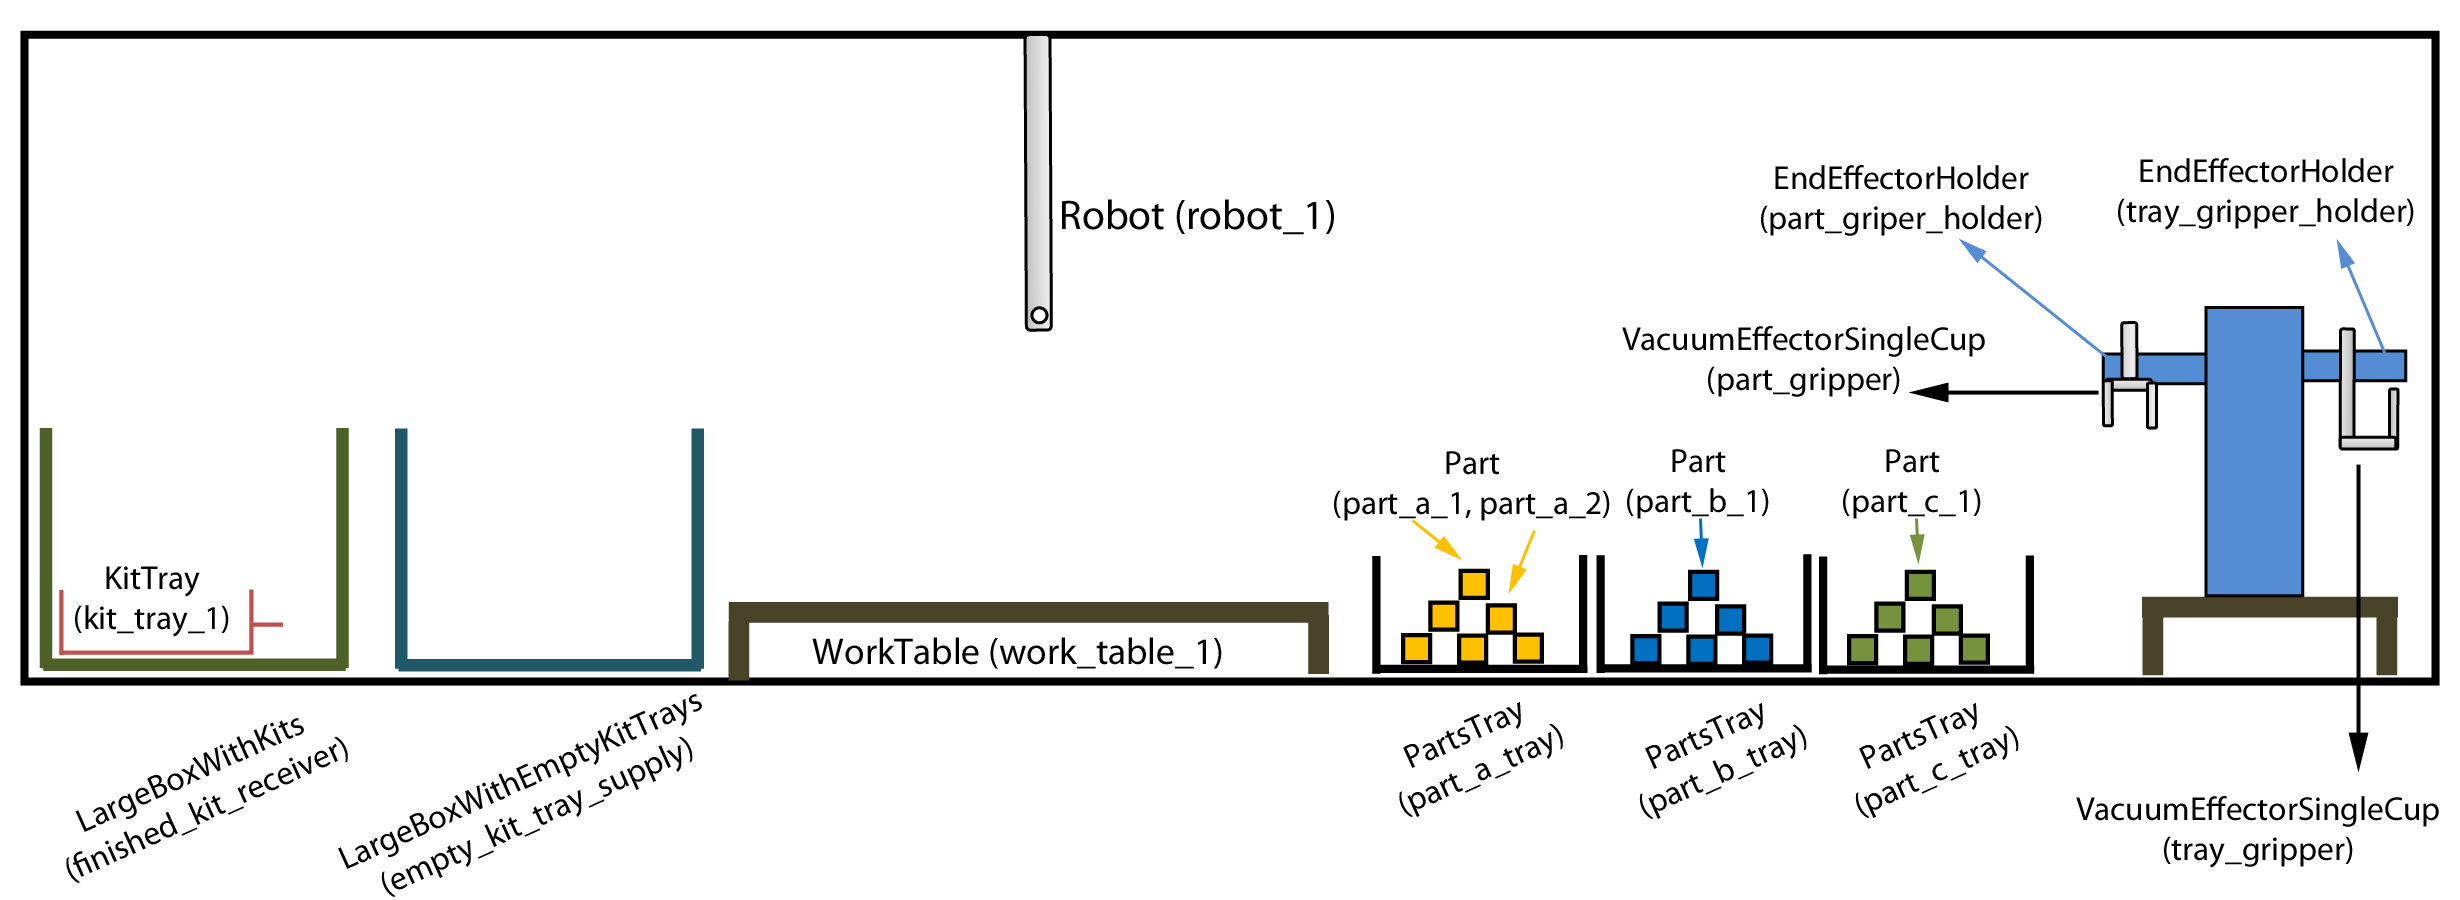
\includegraphics[width=14cm]{Figure/s0.jpg}
\caption{Initial state $S_0$.}
\label{fig:s0}
\end{figure}

\begin{itemize}
\item line 19: \texttt{:init} signals a planner that the predicates and functions in this section are true in the initial state.
\item line 20--87: Predicates true in the initial state of the environment. Since PDDL uses a close world assumption, predicates that are not present in the initial state are automatically set to false. This section also set the initial values for functions. Some relevant sections are presented:
\begin{itemize}
\item line 21: The predicate \stvarsmall{part-not-searched} is set to true so that the operator \op{look-for-part} can be activated during a plan search.
\item line 65--67: Functions describing the quantity of parts of a type that \constsmall{kit\_a2b2c1} can contain. In this example, \constsmall{kit\_a2b2c1} can have 2 parts of type A (\constsmall{part\_a\_tray}), 2 parts of type B (\constsmall{part\_b\_tray}), and 1 part of type C (\constsmall{part\_c\_tray}).
\item line 68--70: Functions that represent the quantity of parts of a specific type that are already in \constsmall{kit\_a2b2c1}. \constsmall{kit\_a2b2c1} has no parts of type A, B, and C.
\item line 71--73: Functions that describe the quantity of parts available in their respective parts tray. This also can be read as: \emph{In the workstation, there are 4 parts of type A available, 4 parts of type B available, and 4 parts of type C available}.
\item line 75--86: Predicates that describe the type of each specific part in the workstation.
\end{itemize}
\end{itemize}

\subsubsection{Goal State}
\begin{figure}[h!t!]
\centering
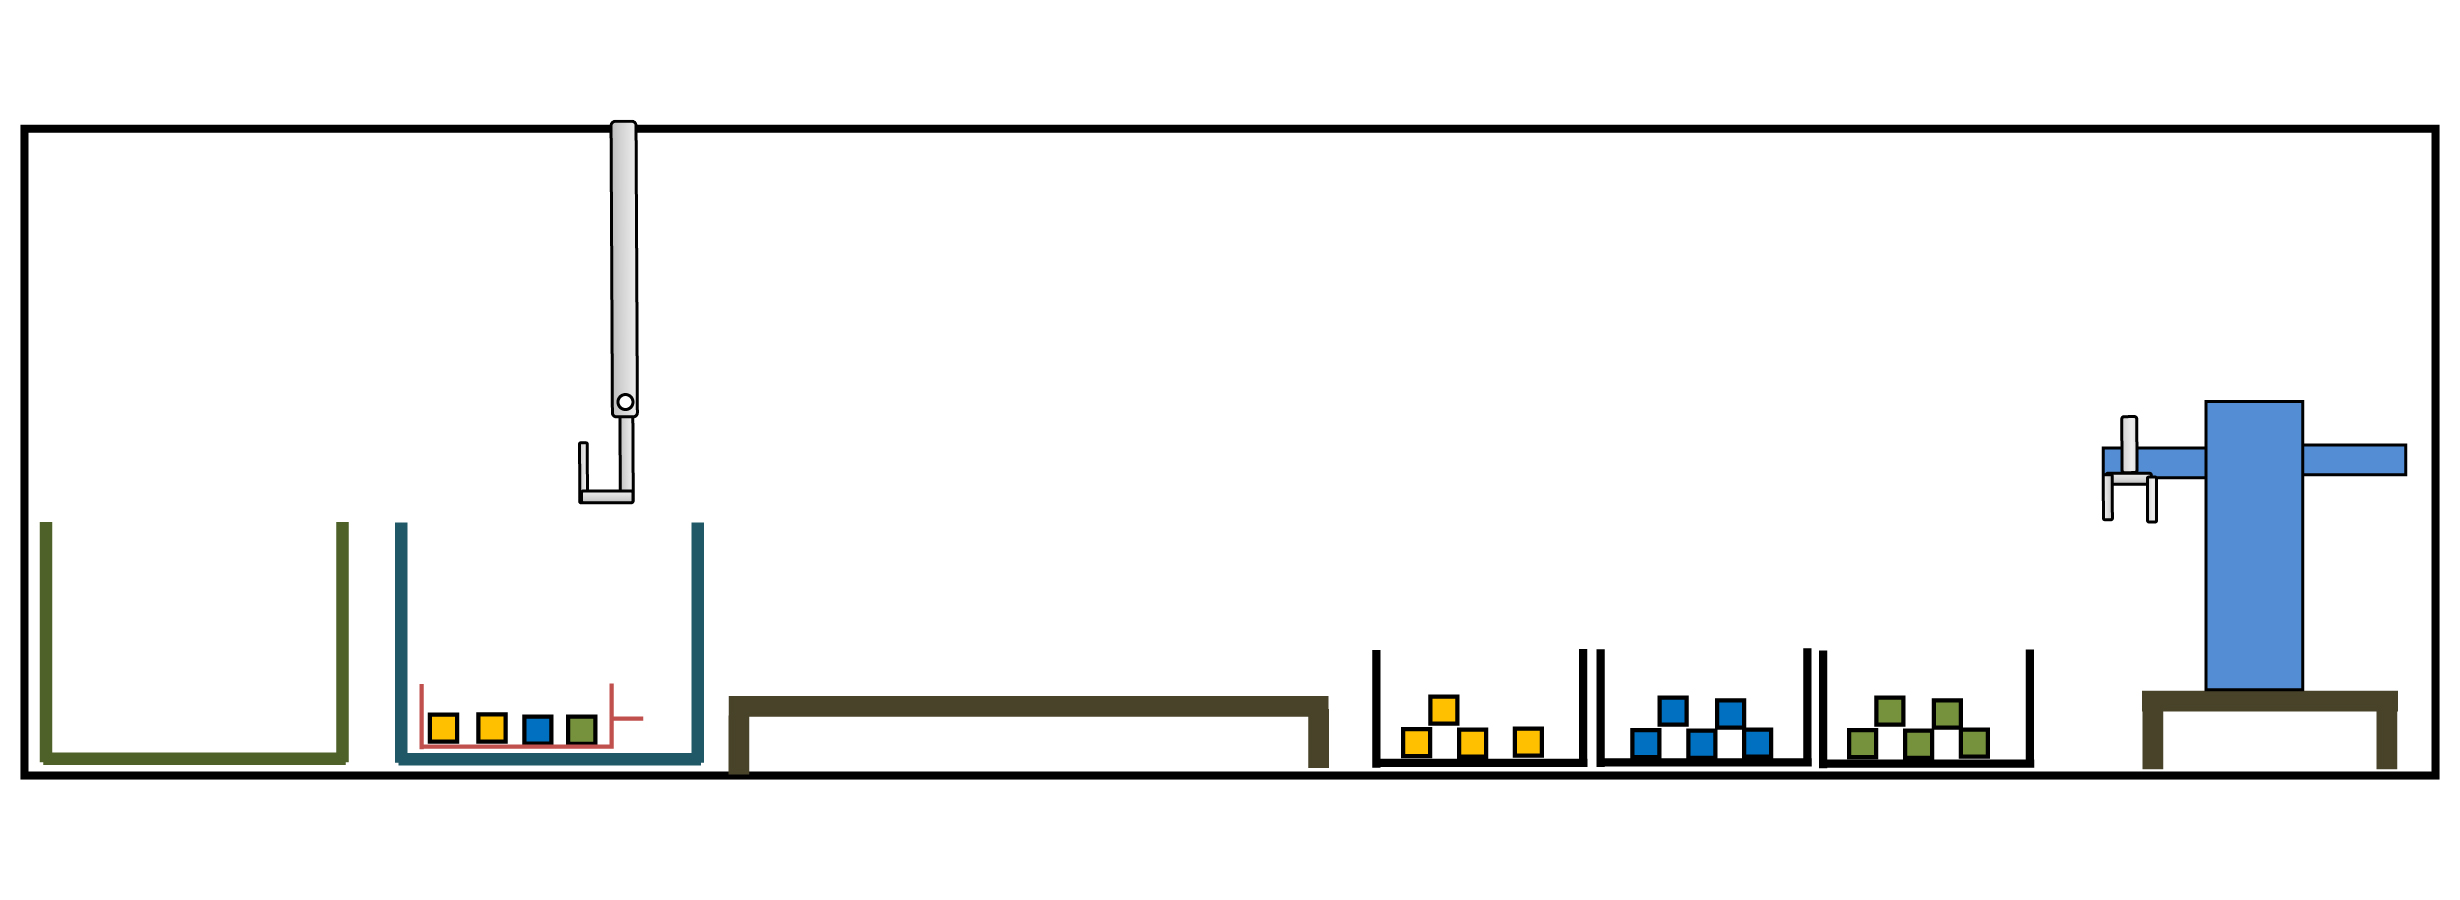
\includegraphics[width=14cm]{Figure/sfinal.jpg}
\caption{Goal state $S_G$.}
\label{fig:sf}
\end{figure}
Figure~\ref{fig:sf} depicts the goal state $S_G$ for the kitting workstation, followed by a representation of the goal state in PDDL format.


\begin{itemize}
\item line 89: \texttt{:goal} is a keyword used to signal a planner about the goal state to reach. All the predicates and functions in the goal state must be true.
\item line 91--93: The quantity of parts of a specific type in \constsmall{kit\_a2b2c1} should match the capacity of parts of a specific type for \constsmall{kit\_a2b2c1}. The quantity of parts in \constsmall{kit\_a2b2c1} is increased in the operator \op{put-part}. The initial quantity of parts in \constsmall{kit\_a2b2c1} and its capacity are set in the initial state. Note that we are not specifying which instance of \class{Part} should go in \constsmall{kit\_a2b2c1} but rather the number of \class{Parts} of a specific type that \constsmall{kit\_a2b2c1} must have.
\item line 94: \constsmall{kit\_a2b2c1} should be placed in the large box with kits \constsmall{finished\_kit\_receiver}.
\end{itemize}

\subsection{Plan}
This section shows an example of plan generated by the planner described in section~\ref{section:planner}. Figure~\ref{fig:plan} displays the different states and actions used by the planner to generate a plan starting from the initial state $S_0$ to the goal state $S_G$. The actions $A_1$ \ldots $A_{17}$ are described below.
\begin{itemize}
\item $A1$:(\opsmall{attach-endeffector} \constsmall{robot\_1} \constsmall{tray\_gripper} \constsmall{tray\_gripper\_holder} \constsmall{changing\_station\_1})
\item $A2$:(\opsmall{take-kittray} \constsmall{robot\_1} \constsmall{kit\_tray\_1} \constsmall{empty\_kit\_tray\_supply} \constsmall{tray\_gripper} \constsmall{work\_table\_1})
\item $A3$:(\opsmall{put-kittray} \constsmall{robot\_1} \constsmall{kit\_tray\_1} \constsmall{work\_table\_1})
\item $A4$:(\opsmall{create-kit} \constsmall{kit\_a2b2c1} \constsmall{kit\_tray\_1} \constsmall{work\_table\_1})
\item $A5$:(\opsmall{remove-endeffector} \constsmall{robot\_1} \constsmall{tray\_gripper} \constsmall{tray\_gripper\_holder} \constsmall{changing\_station\_1})
\item $A6$:(\opsmall{attach-endeffector} \constsmall{robot\_1} \constsmall{part\_gripper} \constsmall{part\_gripper\_holder} \constsmall{changing\_station\_1})
\item $A7$:(\opsmall{look-for-part} \constsmall{robot\_1} \constsmall{part\_c\_1} \constsmall{part\_c\_tray} \constsmall{kit\_a2b2c1} \constsmall{work\_table\_1} \constsmall{part\_gripper})
\item $A8$:(\opsmall{take-part} \constsmall{robot\_1} \constsmall{part\_c\_1} \constsmall{part\_c\_tray} \constsmall{part\_gripper} \constsmall{work\_table\_1} \constsmall{kit\_a2b2c1})
\item $A9$:(\opsmall{put-part} \constsmall{robot\_1} \constsmall{part\_c\_1} \constsmall{kit\_a2b2c1} \constsmall{work\_table\_1} \constsmall{part\_c\_tray})
\item $A10$:(\opsmall{look-for-part} \constsmall{robot\_1} \constsmall{part\_b\_2} \constsmall{part\_b\_tray} \constsmall{kit\_a2b2c1} \constsmall{work\_table\_1} \constsmall{part\_gripper})
\item $A11$:(\opsmall{take-part} \constsmall{robot\_1} \constsmall{part\_b\_2} \constsmall{part\_b\_tray} \constsmall{part\_gripper} \constsmall{work\_table\_1} \constsmall{kit\_a2b2c1})
\item $A12$:(\opsmall{put-part} \constsmall{robot\_1} \constsmall{part\_b\_2} \constsmall{kit\_a2b2c1} \constsmall{work\_table\_1} \constsmall{part\_b\_tray})
\item $A13$:(\opsmall{look-for-part} \constsmall{robot\_1} \constsmall{part\_b\_1} \constsmall{part\_b\_tray} \constsmall{kit\_a2b2c1} \constsmall{work\_table\_1} \constsmall{part\_gripper})
\item $A14$:(\opsmall{take-part} \constsmall{robot\_1} \constsmall{part\_b\_1} \constsmall{part\_b\_tray} \constsmall{part\_gripper} \constsmall{work\_table\_1} \constsmall{kit\_a2b2c1})
\item $A15$:(\opsmall{put-part} \constsmall{robot\_1} \constsmall{part\_b\_1} \constsmall{kit\_a2b2c1} \constsmall{work\_table\_1} \constsmall{part\_b\_tray})
\item $A16$:(\opsmall{look-for-part} \constsmall{robot\_1} \constsmall{part\_a\_2} \constsmall{part\_a\_tray} \constsmall{kit\_a2b2c1} \constsmall{work\_table\_1} \constsmall{part\_gripper})
\item $A17$:(\opsmall{take-part} \constsmall{robot\_1} \constsmall{part\_a\_2} \constsmall{part\_a\_tray} \constsmall{part\_gripper} \constsmall{work\_table\_1} \constsmall{kit\_a2b2c1})
\item $A18$:(\opsmall{put-part} \constsmall{robot\_1} \constsmall{part\_a\_2} \constsmall{kit\_a2b2c1} \constsmall{work\_table\_1} \constsmall{part\_a\_tray})
\item $A19$:(\opsmall{look-for-part} \constsmall{robot\_1} \constsmall{part\_a\_1} \constsmall{part\_a\_tray} \constsmall{kit\_a2b2c1} \constsmall{work\_table\_1} \constsmall{part\_gripper})
\item $A20$:(\opsmall{take-part} \constsmall{robot\_1} \constsmall{part\_a\_1} \constsmall{part\_a\_tray} \constsmall{part\_gripper} \constsmall{work\_table\_1} \constsmall{kit\_a2b2c1})
\item $A21$:(\opsmall{put-part} \constsmall{robot\_1} \constsmall{part\_a\_1} \constsmall{kit\_a2b2c1} \constsmall{work\_table\_1} \constsmall{part\_a\_tray})
\item $A22$:(\opsmall{remove-endeffector} \constsmall{robot\_1} \constsmall{part\_gripper} \constsmall{part\_gripper\_holder} \constsmall{changing\_station\_1})
\item $A23$:(\opsmall{attach-endeffector} \constsmall{robot\_1} \constsmall{tray\_gripper} \constsmall{tray\_gripper\_holder} \constsmall{changing\_station\_1})
\item $A24$:(\opsmall{take-kit} \constsmall{robot\_1} \constsmall{kit\_a2b2c1} \constsmall{work\_table\_1} \constsmall{tray\_gripper})
\item $A25$:(\opsmall{put-kit} \constsmall{robot\_1} \constsmall{kit\_a2b2c1} \constsmall{finished\_kit\_receiver})
\end{itemize}
\begin{figure}[h!]
\centering
\scalebox{.7}{
\begin{tikzpicture}[node distance=1.5cm, every edge/.style={link}]

  %%%%%%%%%%%%%%%%%%%%%%%%%%%%%%%%%%%%%%%%%%%%
  %---------- Main
  %%%%%%%%%%%%%%%%%%%%%%%%%%%%%%%%%%%%%%%%%%%%
  \node[cloud2] (S0)  {$S_0$};
  \node[cloud] (S1) [right=8cm of S0]{$S_1$};
  \node[cloud] (S2) [below=1cm of S1]{$S_2$};
  \node[cloud] (S3) [left=8cm of S2]{$S_3$};
  \node[cloud] (S4) [below=1cm of S3]{$S_4$};
  \node[cloud] (S5) [right=8cm of S4]{$S_5$};
  \node[cloud] (S6) [below=1cm of S5]{$S_6$};
  \node[cloud] (S7) [left=8cm of S6]{$S_7$};
  \node[cloud] (S8) [below=1cm of S7]{$S_8$};
  \node[cloud] (S9) [right=8cm of S8]{$S_9$};
  \node[cloud] (S10) [below=1cm of S9]{$S_{10}$};
  \node[cloud] (S11) [left=8cm of S10]{$S_{11}$};
  \node[cloud] (S12) [below=1cm of S11]{$S_{12}$};
  \node[cloud] (S13) [right=8cm of S12]{$S_{13}$};
  \node[cloud] (S14) [below=1cm of S13]{$S_{14}$};
  \node[cloud] (S15) [left=8cm of S14]{$S_{15}$};
  \node[cloud] (S16) [below=1cm of S15]{$S_{16}$};
  \node[cloud] (S17) [right=8cm of S16]{$S_{17}$};
  \node[cloud] (S18) [below=1cm of S17]{$S_{18}$};
  \node[cloud] (S19) [left=8cm of S18]{$S_{19}$};
  \node[cloud] (S20) [below=1cm of S19]{$S_{20}$};
  \node[cloud] (S21) [right=8cm of S20]{$S_{21}$};
  \node[cloud] (S22) [below=1cm of S21]{$S_{22}$};
  \node[cloud] (S23) [left=8cm of S22]{$S_{23}$};
  \node[cloud] (S24) [below=1cm of S23]{$S_{24}$};
  \node[cloud2] (SG) [right=8cm of S24]{$S_G$};

\draw[myarrow] (S0.east) -- node [above] {$A1$: \opsmall{attach-endeffector}}(S1.west);
\draw[myarrow] (S1.south) -- node [right] {$A2$: \opsmall{take-kittray}}(S2.north);
\draw[myarrow] (S2.west) --  node [above] {$A3$: \opsmall{put-kittray}}(S3.east);
\draw[myarrow] (S3.south) --  node [left] {$A4$: \opsmall{create-kit}}(S4.north);
\draw[myarrow] (S4.east) --  node [above] {$A5$: \opsmall{remove-endeffector}}(S5.west);
\draw[myarrow] (S5.south) --  node [right] {$A6$: \opsmall{attach-endeffector}}(S6.north);
\draw[myarrow] (S6.west) --  node [above] {$A7$: \opsmall{look-for-part}}(S7.east);
\draw[myarrow] (S7.south) --  node [left] {$A8$: \opsmall{take-part}}(S8.north);
\draw[myarrow] (S8.east) --  node [above] {$A9$: \opsmall{put-part}}(S9.west);
\draw[myarrow] (S9.south) --  node [right] {$A10$: \opsmall{look-for-part}}(S10.north);
\draw[myarrow] (S10.west) --  node [above] {$A11$: \opsmall{take-part}}(S11.east);
\draw[myarrow] (S11.south) --  node [left] {$A12$: \opsmall{put-part}}(S12.north);
\draw[myarrow] (S12.east) --  node [above] {$A13$: \opsmall{look-for-part}}(S13.west);
\draw[myarrow] (S13.south) --  node [right] {$A14$: \opsmall{take-part}}(S14.north);
\draw[myarrow] (S14.west) --  node [above] {$A15$: \opsmall{put-part}}(S15.east);
\draw[myarrow] (S15.south) -- node [left] {$A16$: \opsmall{look-for-part}}(S16.north);
\draw[myarrow] (S16.east) -- node [above] {$A17$: \opsmall{take-part}}(S17.west);
\draw[myarrow] (S17.south) -- node [right] {$A18$: \opsmall{put-part}}(S18.north);
\draw[myarrow] (S18.west) -- node [above] {$A19$: \opsmall{look-for-part}}(S19.east);
\draw[myarrow] (S19.south) -- node [left] {$A20$: \opsmall{take-part}}(S20.north);
\draw[myarrow] (S20.east) -- node [above] {$A21$: \opsmall{put-part}}(S21.west);
\draw[myarrow] (S21.south) -- node [right] {$A22$: \opsmall{remove-endeffector}}(S22.north);
\draw[myarrow] (S22.west) -- node [above] {$A23$: \opsmall{attach-endeffector}}(S23.east);
\draw[myarrow] (S23.south) -- node [left] {$A24$: \opsmall{take-kit}}(S24.north);
\draw[myarrow] (S24.east) -- node [above] {$A25$: \opsmall{put-kit}}(SG.west);

\end{tikzpicture}
}
\caption{Example of plan generated with the kitting domain and problem files.}
\label{fig:plan}
\end{figure} 
%\section{Planner}\label{section:planner}
This section describes the steps to install and run a planner on the PDDL domain and problem files in order to generate a plan. The planner uses a forward-chaining partial-order planning~\cite{Coles.ICAPS.2010}.

\subsection{Requirements}
The planner requires:
\begin{itemize}
\item \texttt{cmake}
\item The CBC mixed integer programming solver (\url{https://projects.coin-or.org/Cbc/})
\item \texttt{perl}, \texttt{bison} and \texttt{flex} to build the parser
\end{itemize}

These are packaged with most Linux distributions - on Ubuntu/Debian, the following should suffice:\\

\texttt{sudo apt-get install cmake coinor-libcbc-dev coinor-libclp-dev \textbackslash \\coinor-libcoinutils-dev bison flex}

\subsection{Download and Install CBC}
The CBC source code can be retrieved in two ways:

\begin{enumerate}
\item Local copy: \texttt{ipmas/planner/coin-Cbc.tar.gz}
\item SVN: \footnotesize{\texttt{svn co https://projects.coin-or.org/svn/Cbc/stable/2.8 coin-Cbc}}
\end{enumerate}

If CBC is retrieved using option 1, unzip \texttt{coin-Cbc.tar.gz} to generate the \texttt{coin-Cbc} directory.\\ 

Perform the following steps.
\begin{itemize}
\item \texttt{cd coin-Cbc}
\item \texttt{./configure -C}: Runs a configure script that generates the make file.
\item \texttt{make}: Builds the Cbc library and executable program.
\item \texttt{make test}: Builds and runs the Cbc unit test program.
\item \texttt{make install}: Installs libraries, executables and header files in directories \texttt{coin-Cbc/lib}, \texttt{coin-Cbc/bin} and \texttt{coin-Cbc/include}.
\end{itemize}

\subsection{Compile the Planner}
The planner can be found at \texttt{ipmas/planner/popf2-11jun2011.tar.bz2}. Unzip \texttt{popf2-11jun2011.tar.bz2} to get the \texttt{tempo-sat-popf2} directory, then:
\begin{itemize}
\item cd \texttt{tempo-sat-popf2}
\item \texttt{./build}
\end{itemize}

New files and directories are created in the \texttt{tempo-sat-popf2/compile/} directory. However, the executable is not generated at this point and errors should be displayed. To fix this, open \texttt{tempo-sat-popf2/compile/CMakeCache.txt} in a text editor and edit the following lines. Note that \texttt{<path>} is the absolute path that leads to the \texttt{coin-Cbc} directory.


\begin{itemize}
\item \textbf{line 24}: \texttt{CBC\_INCLUDES:PATH=<path>/include}
\item \textbf{line 33}: \texttt{CGL\_INCLUDES:PATH=<path>/include}
\item \textbf{line 36}: \texttt{CGL\_LIBRARIES:FILEPATH=/usr/lib/libCgl.so.0}
\item \textbf{line 39}: \texttt{CLP\_INCLUDES:PATH=<path>/include}
\item \textbf{line 186}: \texttt{COINUTILS\_INCLUDES:PATH=<path>/include}
\item \textbf{line 230}: \texttt{OSICLP\_LIBRARIES:FILEPATH=/usr/lib/libOsiClp.so.0}
\item \textbf{line 233}: \texttt{OSI\_INCLUDES:PATH=<path>/include}
\item \textbf{line 236}: \texttt{OSI\_LIBRARIES:FILEPATH=/usr/lib/libOsi.so.0}
\end{itemize}

Recompile the planner:\\
\texttt{./build}


\subsection{Run the Planner}
To run the planner, the path to the PDDL domain and problem files should be identified. The format of the PDDL files must be \texttt{.pddl}. The following command run the planner on the PDDL files.

\begin{itemize}
\item \texttt{./plan <domain> <problem> <solution>}
\end{itemize}


Where \texttt{<domain>} and \texttt{<problem>} are the paths that point to the PDDL domain and problem files, respectively.\\\texttt{<solution>} is the output file that will contain the plan.

%\section{Tools}\label{tools}


%%%%%%%%%%%%%%%%%%%%%%%%%%%%%%%%%%%%%%%%%%%
\subsection{The Generator}\label{generator}
%%%%%%%%%%%%%%%%%%%%%%%%%%%%%%%%%%%%%%%%%%%
The Generator tool is a graphical user interface developed in Java, allowing the user to store data from OWL files into a MySQL database. This tool also permits the user to query the database using the C++ function calls. The tool Generator is composed of the following functionalities:
\begin{enumerate}
 \item Convert OWL documents into SQL syntaxes (OWL to SQL).
 \item Translate SQL syntaxes to OWL language in order to modify an OWL document (SQL to OWL).
 \item Convert the OWL language into C++ classes (OWL to C++).
\end{enumerate}

To date, only steps 1. and 3. have been implemented and will be covered in this document.

\subsubsection{Prequisites}\label{s:prequisites}
The description of the Generator tool is given for a Ubuntu Linux system. To run and use the Generator tool, different applications must be installed on the system.

\paragraph{Java Runtime Environment}
The Generator tool comes as a jar file. As such, the Java Runtime Environment should be installed on your system. This application can be found at \url{www.oracle.com}.

\paragraph{MySQL Server and Client}
The MySQL server and client should be installed and running on your system.
\begin{itemize}
 \item \textit{sudo apt-get update} (Update the package management tools)
 \item \textit{sudo apt-get dist-upgrade} (Install the latest software)
 \item \textit{sudo apt-get install mysql-server mysql-client} (Install the MySQL server and client packages). You will be asked to enter a password.
\end{itemize}

When done, you have a MySQL database ready to run. The following command will allow you to run MySQL.

\begin{itemize}
 \item \textit{mysql -u root -p}
 \item Enter the same password you used when you installed MySQL.
\end{itemize}

Finally, we need the plugin \texttt{libmysqlcppconn-dev} which allows C++ to connect to MySQL databases. It can be installed as follows:
\begin{itemize}
 \item \textit{sudo apt-get install libmysqlcppconn-dev}
\end{itemize}

\subsubsection{How to Run the Generator Tool}\label{s:run}
The Generator tool can be launched using either one of these two following methods:
\begin{enumerate}
 \item \textit{java -jar Generator.jar}
 \item Right-click on Generator.jar and select the option ``Open With OpenJDK Java 6 Runtime". Note that this message will be different for future releases of the Java Runtime Environment.
\end{enumerate}


\subsubsection{Functionalities}\label{s:generator}
As mentioned in the Introduction, we are covering only steps 1. and 3. in the rest of this document, i.e., \textit{OWL to SQL} and \textit{OWL to C++}, respectively.

\paragraph{OWL to SQL}
\begin{figure}[h!t!]
\centering
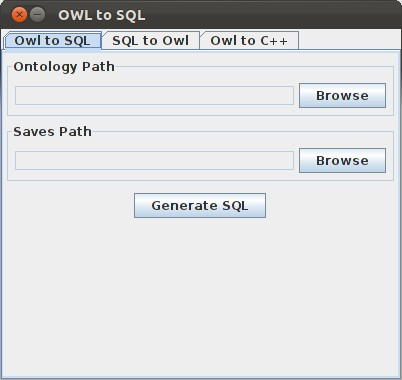
\includegraphics[width=9cm]{Figure/OWLtoSQL001.jpeg}
\caption{Owl to SQL tab.}
\label{fig:owl2sql}
\end{figure}
To convert OWL classes and instances to SQL, the \texttt{Owl to SQL} tab should be selected (see Figure~\ref{fig:owl2sql}). The different fields are:

\subparagraph{Generate SQL Files}
\begin{itemize}
 \item Ontology Path: This field requires the file \texttt{kittingInstances.owl}. Before doing so, you need to modify one line in this file. Open it with a text editor and find the line \texttt{Import(<file:kittingClasses.owl>)}. Modify
this line by giving the absolute path to the file \texttt{kittingClasses.owl}. You should should have something that looks like \texttt{Import(<file:/home/username/NIST/ipmas/Generator/kittingClasses.owl>)}. When this is done, save the file, and browse to  \texttt{kittingInstances.owl} using the ``Browse" button.
 \item Browse to the directory where you want to save the SQL files.
\end{itemize}

Once the two previous steps are done, click on ``Generate SQL''. You should receive a message confirming the generation of the SQL files: \texttt{kittingInstances.owlCreateTable.sql} and \texttt{kittingInstances.owlInsertInto.sql}. The former is used to create tables, the latter is used to populate these tables;

\subparagraph{SQL Tables and Insertions}
The next step is to create a database and to populate it.

\begin{itemize}
\item Connect to mysql using \textit{mysql -u root -p}, then enter your password. You should be in the mysql shell if this succeeded (\textit{mysql>}).
\item Delete a previous database (if you already used this tool and you want to replace the existing database with this new one) :
\texttt{mysql>} \textit{DROP DATABASE OWL;} (\textit{OWL} is the name of the old database).
\item Create a database:
\begin{itemize}
\item \texttt{mysql>} \textit{CREATE DATABASE OWL;}. Here, \textit{OWL} is the name of the database (you can use a name of your choice).
\item Before performing the following commands, we need to tell MySQL which database we are planning to work with (\textit{OWL} in our case). This is done using:
\begin{itemize}
\item[] \texttt{mysql>} \textit{USE OWL}
\end{itemize}
\end{itemize}
\item Populate the database with tables using \texttt{kittingInstances.owlCreateTable.sql}.
\begin{itemize}
 \item \texttt{mysql>} \textit{source <path>/kittingInstances.owlCreateTable.sql;}
\end{itemize}

\item Populate the tables with data using \texttt{kittingInstances.owlInsertInto.sql}:
\begin{itemize}
 \item \texttt{mysql>} \textit{source <path>/kittingInstances.owlInsertInto.sql;}
\end{itemize}
\end{itemize}

\textit{<path>} designs the absolute path to the appropriate file.

\paragraph{OWL to C++}
\begin{figure}[h!t!]
\centering
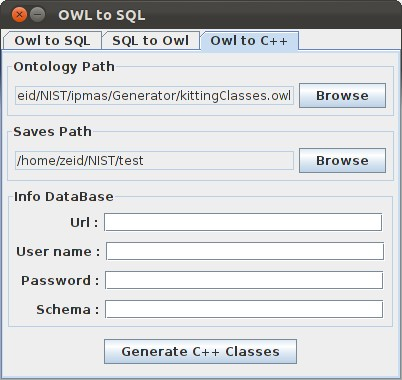
\includegraphics[width=9cm]{Figure/OWL2C++.jpeg}
\caption{Owl to C++ tab.}
\label{fig:owl2C++}
\end{figure}
The ``Owl to C++" tab (see Figure~\ref{fig:owl2C++}) is used to generate C++ classes and scripts allowing the connection between C++ and MySQL. The different fields are explained below:
\begin{itemize}
\item \textbf{Ontology Path}: This is the path to the ontology (\texttt{kittingClasses.owl} in our example).
\item \textbf{Saves Path}: Directory where the C++ files and scripts will be generated.
\item \textbf{Url}: This is the url of the database. It's usually the IP address of the machine hosting the database (127.0.0.1 if it is local).
\item \textbf{User name}: User name used to connect to the MySQL database.
\item \textbf{Password}: Password associated to the user name to connect to the MySQL database.
\item \textbf{Schema}: This is the name of the database (\textit{OWL} in our example).
\end{itemize}

When all the fields are completed, click the ``Generate C++ Classes" button to generate C++ and script files.

%%%%%%%%%%%%%%%%%%%%%%%%%%%%%%%%%%%%%%%%%%%
\subsection{XML to OWL}\label{xml2owl}
%%%%%%%%%%%%%%%%%%%%%%%%%%%%%%%%%%%%%%%%%%%
This section describes tools that are used to generate OWL files from XML files.
\subsubsection{owlPrinter}
owlPrinter reads an XML kitting data file corresponding to an XML schema for kitting (\file{kitting.xsd}) and writes an OWL instance file corresponding to the OWL class file \file{kittingClasses.owl}. The \file{kitting.xsd} file contains the same conceptual model as the \file{kittingClasses.owl} file, but in a different language.

The owlPrinter is useful because there is no OWL tool that will help generate an OWL instance file and check the file adequately against an OWL class file. That is because OWL uses an open world model in which anything not explicitly or implicitly illegal is allowed. Hence many things that are errors to the writer of the instance file are not OWL errors. For example, if the name of an instance is misspelled, OWL will assume that there is a new instance that has not been explicitly declared as such, which is OK in OWL. If a reference to an instance name is misspelled in an XML data file corresponding to the \file{kitting.xsd} schema, that will be caught automatically by the owlPrinter (and other readily available XML tools).  Several other types of error will not be caught by OWL tools but will not be made or will be detected if the OWL printer is used.

Another OWL problem that disappears in XML is that in OWL, there is no distinction between an instance file and a class file. An instance file can modify classes, intentionally, or accidentally. In XML there is no way a data file can modify a model.

To use the owlPrinter, use a text editor such as emacs or an XML tool such as XMLSpy to write an XML data file corresponding to the \file{kitting.xsd} schema and then run it through the owlPrinter with a command of the form:\\

\texttt{bin/owlPrinter [XML file in] [OWL file out]}\\

For example, the command\\

\texttt{bin/owlPrinter data/kittingInstances.xml junk}\\

will print the file junk, which will be identical to the \file{kittingInstances.owl} file in the owl directory (except for a couple comments).


\subsubsection{kittingParser}
The kittingParser may be used to check an XML data file against the
kitting.xsd schema. The schema is hard-coded into the kittingParser.
If there is any error in the XML data file, the kittingParser prints
a message and quits. If there is no error, the input file is echoed by
printing an output file whose name is the same as that of the input file
with "echo" appended. To run the kittingParser, give a command of the
form:\\
\texttt{bin/kittingParser [XML kitting data file in]}\\

For example, the command\\

\texttt{bin/kittingParser data/kittingInstances.xml}

will read \file{kittingInstances.xml} and write \file{kittingInstances.xmlecho}. The
two files will be identical except for comments. If the format of an
input file differs from the format used for printing the output file,
the two files will differ, but only in format.

The owlPrinter makes the same checks as the kittingParser, so there is
no need to use the kittingParser.

All of the source code for the kittingParser was generated automatically
by the GenXMiller generator.

\subsubsection{compactOwl and compareOwl}
There is no need to read this section unless you are interested in how the
\app{owlPrinter} was debugged.

The \app{compactOwl} and \app{compareOwl} utilities are used for checking that two
different OWL instance files have the same statements. They have been
used as follows to debug the \app{owlPrinter} (and the \file{kitting.xsd} file
and the \file{kittingInstances.xml} file and the \file{kittingInstances.owl} file).

\begin{enumerate}
\item Write \file{kitting.xsd} to model the same information as \file{kittingClasses.owl}.

\item Write \file{kittingInstances.xml} to correspond to \file{kitting.xsd} and contain the
same information as \file{kittingInstances.owl}.

\item Build the \app{owlPrinter}.

\item Run \file{kittingInstances.xml} through the \app{owlPrinter} to produce
\file{kittingInstances.owl}.

\item Run \file{kittingInstances.owl} through \app{compactOwl} to produce
one version of \file{kittingInstancesCompact.owl}.

\item Run \file{kittingInstances.owl} through \app{compactOwl} to produce
a second version of \file{kittingInstancesCompact.owl}.

\item Run the two versions of \file{kittingInstancesCompact.owl} through
\app{compareOwl}. If \app{compareOwl} reports that the two files have the same
statements, that means that steps 1, 2, and 3 have been done correctly, so
debugging is finished. If \app{compareOwl} reports a pair of statements that
differ, figure out why, go back to step 1, 2, or 3 (or edit
\file{kittingInstances.owl}), fix the problem, and repeat the subsequent steps.
\end{enumerate}

These utilities assume that the format of the input files is the same
as either the format used by the \app{owlPrinter} or the format followed by
the \file{kittingInstances.owl} file. If the format used by an input file is
different from both of those, the utilities may fail.

The \app{compactOwl} utility compacts an OWL instance file by:
\begin{enumerate}
\item removing all occurrences of one or two blank lines. The blank lines
   must not contain spaces or tabs.
\item removing comments. The comments must have ``//'' as the first two
   characters on the line.
\item combining each OWL statement written on two or more lines so it is
   all on one line. The first non-space character on the second line
   must be a colon (:) or a double quote (").
\item rewriting numbers with decimal points so there are exactly six decimal
   places. Such numbers must have at least one digit on each side of the
   decimal point in the input file.
\item putting the \textbf{DifferentIndividuals} inside \textbf{DifferentIndividuals} statements
   into alphabetical order.
\end{enumerate}
To run \app{compactOwl} use a command of the form:\\

\texttt{bin/compactOwl < [owl file in] > [owl file out]}\\

where \texttt{[owl file in]} and \texttt{[owl file out]} are replaced by file names.

The \app{compareOwl} utility compares two files that are expected to have the
same lines, but in a different order, such as an automatically generated
OWL file and a hand-written OWL file. It reads the two files and saves the
lines of each one in two sets in alphabetical order (set::insert puts
strings in alphabetical order by default). Then it compares the lines of
the two sets in order. If it finds two lines that do not match, it prints
the line from the first file followed by the line from the second file.  If
all lines match, that is reported.

To run \app{compareOwl}, use a command of the form:\\

\texttt{bin/compareOwl [first owl file in] [second owl file in]}

where \texttt{[first owl file in]} and \texttt{[second owl file in]} are replaced by the
names of compacted OWL files.

% File:   authindx.tex
% Author: Zeid Kootbally
% Update: 2008-10-3
% Info:   references - part of PhD

\cleardoublepage
\bibliographystyle{plain}
\small{
\bibliography{bib/kitting-ref}
} \clearpage{\pagestyle{empty}\cleardoublepage}
 % References

\setcounter{lofdepth}{2} \listoffigures
%% File:   subjindx.tex
% Author: Zeid Kootbally
% Update: 2008-10-3
% Info:   subject index - part of PhD


%\chapter*{Subject Index}
\markboth{Subject Index}{Subject Index}
\addcontentsline{toc}{chapter}{Subject Index}
\printindex[def]
 % subject index
\setcounter{lofdepth}{2} \listoftables
%\include{Chapters/authindx} % author index

\end{document}


%%%%%%%%%%%%%%%%%%%%%%%%%%%%%%%%%%%%%%%%%%%%%%%%%%%%%%%%%%%%%%%%%%%%%%%%%
\section{Ontology}
\label{Sect:Ontology}
We believe that building models of the world knowledge is a necessary step towards operating an automated kitting workstation. The proposed models include representations for non-executable information about the kitting workstation such as information about parts, kits, and trays. The description of these models includes for instance the location, orientation, and relation between components. These models are discussed in Section~\ref{owlkitting}. Models of executable information are also produced from the system information described in the SVR. These models include actions along with their precondition and effect, and failures. Section~\ref{owlsoap} discusses models of executable information.

Models for non-executable and executable information can be combined to generate the OWL/XML kitting \onto{init} and \onto{goal} conditions files, as described in Section~\ref{owlinitgoal}.

%+++++++++++++++++++++++++++++++++++++++++++++++++++++++++++%
\subsection{The OWL/XML Kitting Ontology}\label{owlkitting}
%+++++++++++++++++++++++++++++++++++++++++++++++++++++++++++%
In order to maintain compatibility with the IEEE Robotics and Automation Society's Ontologies for
Robotics and Automation Working Group, the \onto{Kitting} ontology has been fully defined in the Web Ontology Language (OWL)~\cite{OWLoverview}. In addition, the ontology was also fully defined in the XML schema language~\cite{Walmsley.2002}. Although the two models are conceptually identical, there are some systematic differences between the models (in addition to differences inherent in using two different languages) that are discussed in Balakirsky~\textit{et al.}~\cite{Balakirsky.whitepaper.2012}.
%
%\begin{itemize}
%  \item The \textsf{complexType} names (i.e. class names) in XML schema have the suffix ``Type" added which is not used in OWL. This is so that the same names without the suffix can be used in XML schema language as element names without confusion.
%  \item All of the XML schema \textsf{complexTypes} have a ``Name" element that is not present in OWL. It is not needed in OWL because names are assigned as a matter of course when instances of classes are created.
%  \item The XML schema model has a list of ``Object" elements. This collects all of the movable objects. The OWL model does not have a corresponding list. In an OWL data file, the movable objects may appear anywhere.
%  \item OWL has classes but does not have attributes; it has \textsf{ObjectProperties} and \textsf{DataProperties} instead. They may be used to model attributes. OWL Properties are global, not local to a class, so localizing each attribute to a class is done by a naming convention that includes using prefixes as described below. The prefixes are not used in XML schema.
%  \item OWL supports multiple inheritances, but that has not been used in the \onto{Kitting} ontology. Except by subclass relationship, no object is in more than one class.
%\end{itemize}

\begin{table}[h!t!b!]
  \caption{Excerpt of the \onto{Kitting} ontology.}
  \label{tab:kittingonto}
  \centering
  \begin{tabular}{l}
    \hline
    \class{SolidObject} \textit{PrimaryLocation} \textit{SecondaryLocation}
    \\\hline
    \hspace{5 mm}\class{Kit} \textit{Tray} \textit{DesignRef} \textit{Parts} \textit{Finished?}
    \\\hline
    \hspace{5 mm}\class{LargeBoxWithEmptyKitTrays} \textit{LargeContainer} \textit{Trays}
    \\\hline
    \hspace{5 mm}\class{LargeBoxWithKits} \textit{LargeContainer} \textit{Kits} \textit{KitDesignRef} \textit{Capacity}
    \\\hline
    \hspace{5 mm}\class{PartsTrayWithParts} \textit{PartTray}
    \\\hline
    \hspace{5 mm}\ldots
    \\\hline
    \class{DataThing}
    \\\hline
    \hspace{5 mm}\class{PhysicalLocation} \textit{RefObject}
    \\\hline
    \hspace{10 mm}\class{PoseLocation} \textit{Point} \textit{XAxis} \textit{ZAxis}
    \\\hline
    \hspace{15 mm}\class{PoseLocationIn}
    \\\hline
    \hspace{15 mm}\class{PoseLocationOn}
    \\\hline
    \hspace{10 mm}\class{RelativeLocation} \textit{Description}
    \\\hline
    \hspace{15 mm}\class{RelativeLocationIn}
    \\\hline
    \hspace{15 mm}\class{RelativeLocationOn}
    \\\hline
    \hspace{5 mm}\ldots
    \\\hline
  \end{tabular}
\end{table}

\class{SolidObject} and \class{DataThing} constitute the two top-level classes of the \onto{Kitting} ontology model, from which all other classes are derived. \class{SolidObject} models solid objects, things made of matter. The \onto{Kitting} ontology includes several subclasses of \class{SolidObject} that are formed from
components that are \class{SolidObject}. The \class{DataThing} class models data for \class{SolidObject}. Examples of subclasses for \class{SolidObject} and \class{DataThing} are represented in Table~\ref{tab:kittingonto}. Items in italics following classes are names of class attributes. Derived types inherit the attributes of the parent. Each attribute has a specific type not shown in Table~\ref{tab:kittingonto}. If an attribute type has derived types, any of the derived types may be used.

Using Table~\ref{tab:kittingonto}, an example of interaction between classes \class{SolidObject} and \class{DataThing} can be expressed as follows: Each \class{SolidObject} \class{A} has at least one \class{PhysicalLocation} (the \textit{PrimaryLocation}). A \class{PhysicalLocation} is defined by giving a reference \class{SolidObject} \class{B} (\textit{RefObject}) and information saying how the position of \class{A} is related to \class{B}. \class{PhysicalLocation} consists of two types of location which are required for the operation of the kitting workstation:
\begin{itemize}
 \item Mathematically precise locations are needed to support robot motion. The mathematical location, \class{PoseLocation}, gives the pose of the coordinate system of \class{A} in the coordinate system of \class{B}. The mathematical information consists of the location of the origin of \class{A}'s coordinate system (\textit{Point}) and the directions of its Z (\textit{ZAxis}) and X (\textit{XAxis}) axes. The mathematical location variety has subclasses representing that, in addition, \class{A} is in \class{B} (\class{PoseLocationIn}) or on \class{B} (\class{PoseLocationOn}).
\item Relative locations (class \class{RelativeLocation}), specifically the knowledge that one \class{SolidObject} is in (\class{RelativeLocationIn}) or on (\class{RelativeLocationOn}) another, are needed to support making logical plans for building kits. The subclasses of \class{RelativeLocation} are needed not only for
logical planning, but also for cases when the relative location is known, but the
mathematical information is not available.
\end{itemize}


%++++++++++++++++++++++++++++++++++++++++++++++++++++++%
\subsection{The OWL/XML SOAP Ontology}\label{owlsoap}
%++++++++++++++++++++++++++++++++++++++++++++++++++++++%
As depicted in Figure~\ref{fig:DesignArchitecture}, the \onto{SOAP} ontology imports the \onto{Kitting} ontology. The \onto{Kitting} ontology is involved in the process that generates the PDDL domain file and in the process that evaluates the truth-value of predicates. While some concepts in the \onto{SOAP} ontology are used by both processes, other concepts are exclusive to one of these two processes. We approach the description of the \onto{SOAP} ontology with a discussion on each process.

%------------------------------------------------------------------------------------------------------------------------------%
\subsubsection{PDDL Domain File Generator Process}\label{sss:domainfile}
%------------------------------------------------------------------------------------------------------------------------------%
A PDDL domain file consists of definitions of actions, predicates, and functions. Actions are ways of changing the state of the world and consist of a precondition and an effect sections. Predicates and functions constitute preconditions and effects. Predicates are used to encode Boolean state variables while functions are used to model updates of numerical values. Introducing functions into planning makes it possible to model actions in a more compact and sometimes more natural way~\cite{FOX.JAIR.2003}. Both predicates and functions are well documented in the SVR. Figure~\ref{fig:put-part} shows the action \textsl{put-part} that will be used as the model to discuss the components of a PDDL action.

\begin{figure}[t!h!]
\begin{minipage}{.5\paperwidth}
\begin{list}{}{\setlength{\leftmargin}{1em}}\item\small
\begin{Verbatim}[commandchars=\\\{\},fontsize=\scriptsize, numbers=left, numbersep=2pt]
(:action put-part
   :parameters(
      ?robot - Robot
      ?part - Part
      ?kit - Kit
      ?worktable - WorkTable
      ?partstray - PartsTray)
   :precondition (and
      (part-location-robot ?part ?robot)
      (robot-holds-part ?robot ?part)
      (on-worktable-kit ?worktable ?kit)
      (origin-part ?part ?partstray)
      (< (quantity-kit ?kit ?partstray)
      (capacity-kit ?kit ?partstray))
      (kit-location-worktable ?kit ?worktable))
   :effect (and
      (not (part-location-robot ?part ?robot))
      (not (robot-holds-part ?robot ?part))
      (part-not-searched)
      (not (found-part ?part ?partstray))
      (part-location-kit ?part ?kit)
      (increase (quantity-kit ?kit ?partstray) 1)
      (robot-empty ?robot))
)
\end{Verbatim}
\end{list}
\end{minipage}
\caption{PDDL action put-part.}
\label{fig:put-part}
\end{figure}

\begin{enumerate}
  \item \texttt{action} (line 1): The unique name of the action comes directly after the keyword \texttt{:action}. In this example, the name of the action is \texttt{put-part}.
  \item \texttt{parameters} (lines 2--7): The parameters (preceded by a ? mark) that participate in this action are listed along their types. For example, line 3 can be read as ``\texttt{robot} is a parameter and is of type \texttt{Robot}''.
  \item \texttt{precondition} (lines 8--15): List of all the predicates and functions needed in the precondition section.
  \item \texttt{effect} (lines 16--23): List of all the predicates and functions needed in the effect section.
\end{enumerate}

The representation of PDDL action in the ontology is made up of the classes \class{Action}, \class{Precondition}, \class{Effect}, \class{Predicate}, \class{Function}, \class{ParameterList}.  Operations between functions such as the one shown at lines 13--14 in Figure~\ref{fig:put-part}, are expressed with the class \class{FunctionBool}. All these classes are subclasses of \class{DataThing}.

In the remainder of this section, we provide paragraph descriptions of each of the classes used to represent PDDL actions in the \onto{SOAP} ontology. The naming convention utilized below follows the OWL implementation of the ontology.

\begin{enumerate}
\item \class{Action} -- An \class{Action} has a \class{Precondition} (\emph{hasAction\_Precondition}) and an \class{Effect} (\emph{hasAction\_Effect}). An \class{Action} has a \class{ParameterList} (\emph{hasAction\_ParameterList}) that contains all the parameters for a PDDL action. As seen in Figure~\ref{fig:put-part}, an action has unique name (\emph{hasAction\_Name}) of type \texttt{string}.
\item \class{ParameterList} -- The \textsl{put-part} action illustrated in Figure~\ref{fig:put-part} has five parameters of different types. Each one of these types is represented by a class in the \onto{Kitting} ontology. To represent all PDDL actions in the \onto{SOAP} ontology, we considered all the different types of parameters that are used in all our ten PDDL actions. To date, we are using eleven different types of parameter, represented by the eleven following classes: \class{Robot}, \class{EndEffectorChangingStation}, \class{KitTray}, \class{Kit}, \class{LargeBoxWithEmptyKitTrays}, \class{LargeBoxWithKits}, \class{WorkTable}, \class{PartsTray}, \class{Part}, \class{EndEffector}, and \class{EndEffectorHolder}. Therefore, \class{ParameterList} has at least a parameter (\emph{hasAction\_Parameter}) that is from one of these eleven classes.
    
    The order of the parameters in a PDDL action also needs to be represented in the ontology. In Figure~\ref{fig:put-part}, the parameter \texttt{robot} comes before the parameter \texttt{part}, the parameter \texttt{part} comes before the parameter \texttt{kit}, and so on. OWL has no built-in structure to represent an ordered list, instead, all the eleven classes mentioned earlier, use \emph{hasParameter\_Next} to point to the next parameter in \class{ParameterList}.
\item \class{Precondition} -- A \class{Precondition} can consist of only one \class{Predicate} (\emph{hasPrecondition\_Predicate}), only one \class{Function} (\emph{hasPrecondition\_Function}), \class{FunctionBool} (\emph{hasPrecondition\_FunctionBool}), or a combination of these three classes. A \class{Precondition} belongs to one \class{Action} (\emph{hadByPrecondition\_Action}).
\item \class{Effect} -- An \class{Effect} can consist of only one \class{Predicate} (\emph{hasEffect\_Predicate}), only one \class{Function} (\emph{hasEffect\_Function}), \class{FunctionBool} (\emph{hasEffect\_FunctionBool}), or a combination of these three classes. An \class{Effect} belongs to one \class{Action} (\emph{hadByEffect\_Action}). A negative \class{Predicate} is represented with the declaration of \emph{hasEffect\_Predicate} within the OWL built-in property assertion \texttt{owl:NegativePropertyAssertion}.
\item \class{Predicate} -- A \class{Predicate} has a unique name (\emph{hasPredicate\_Name}) of type \texttt{string}. A \class{Predicate} has a reference parameter (\emph{hasPredicate\_RefParam}) and a target parameter (\emph{hasPredicate\_TargetParam}). A reference parameter is the first parameter in the \class{Predicate}'s list and the target parameter is the second parameter in the parameter's list. A \class{Predicate} cannot have more than two parameters due to the definition of \class{Predicates} in the SVR. In the case a \class{Predicate} has only one parameter, it is assign to the reference parameter. Reference and target parameters are one of the parameters defined for the \class{Action} to which the \class{Predicate} belongs.
\item \class{Function} -- A \class{Function} has a unique name (\emph{hasFunction\_Name}) of type \texttt{string}. A \class{Function} has a reference parameter (\emph{hasFunction\_RefParam}) and a target parameter (\emph{hasFunction\_TargetParam}). The same rules apply to the definition and use of these two types of parameters as the ones defined for \class{Predicate}.
\item \class{FunctionBool} -- \class{FunctionBool} has one or more subclasses that represent the type of relation between two \class{Functions}. For example, the relation depicted at line 13--14 in Figure~\ref{fig:put-part} is represented in the subclass \class{IntLesserThanInt}. Subclasses of \class{FunctionBool} have a first \class{Function} (\emph{hasFunctionBool\_FirstFunction}) that represents the \class{Function} on the left side of the operator. Subclasses of \class{FunctionBool} have a second \class{Function} (\emph{hasFunctionBool\_SecondFunction}) that represents the \class{Function} on the right side of the operator.
\end{enumerate}

%-------------------------------------------------------------%
\subsubsection{Concepts for Action Failure}\label{sss:failure}
%-------------------------------------------------------------%
 A failure is any change or any design or manufacturing error that renders a component, assembly, or system incapable of performing its intended function. In kitting, failures can occur for multiple reasons: equipment not set up properly, tools and/or fixtures not properly prepared, lack of safety, and improper equipment maintenance. Part/component availability failures can be triggered by inaccurate information on the location of the part, part damage, wrong type of part, or part shortage due to delays in internal logistics. In order to prevent or minimize failures, a disciplined approach needs to be implemented to identify the different ways a process design can fail before impacting the productivity. 
 
 Failures detected in the workstation can result in the current plan to become obsolete. When a failure is detected in the execution process and the failure mode identified, the value of the severity for the failure mode will be retrieved from the ontology and the appropriate contingency plan will be activated. In some cases, the current state of the environment is brought back to the state prior to the failure and the robot starts from a ``stable" state. To select the right contingency plan, i.e., the less time consuming or safer, the system will need to rely on the information from the knowledge representation.
 
 In the knowledge driven diagram (Figure~\ref{fig:DesignArchitecture}), the \process{Predicate Evaluation} process is responsible for failure detection. An action failure consists of failure modes that can occur during the execution of a PDDL action. The steps to identify action failures in the kitting system are described in Figure~\ref{fig:algo}.

\begin{figure}[h!t!]
  \centering
  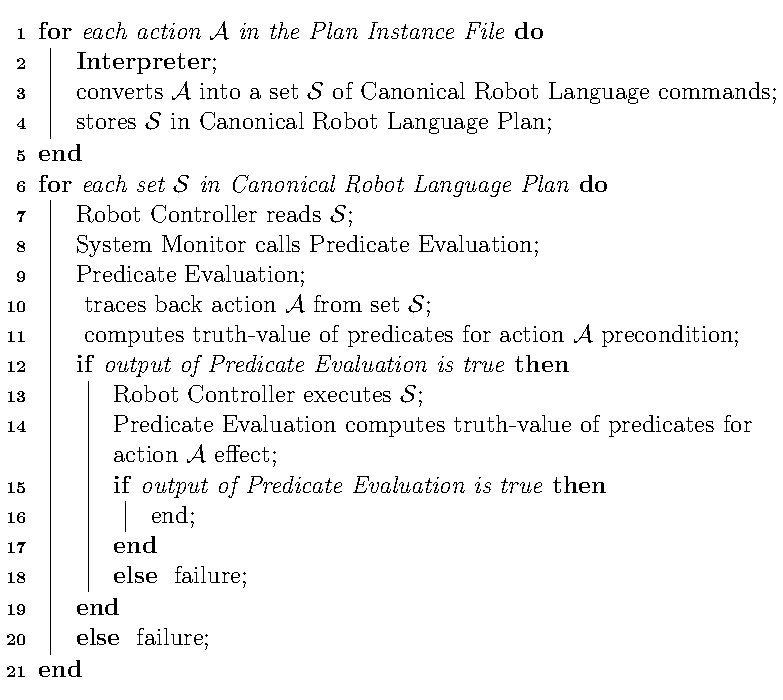
\includegraphics[width=10cm]{images/algorithm.pdf}
  \caption{Failure identification.}
  \label{fig:algo}
\end{figure}

As seen in Figure~\ref{fig:algo}, failures are identified during the execution of canonical robot commands (line 6), generated from PDDL actions (line 3) by the \process{Interpreter}. The \process{Predicate Evaluation} process outputs a Boolean value that results in a failure detection if this value is false (lines 18 and 20). Therefore, to represent failures in the \onto{SOAP} ontology, the following concepts are introduced:
\begin{itemize}
 \item ``Action'' the PDDL action for which a failure can occur.
 \item ``Failure Modes'': List of failure modes that can occur during the execution of a specific action.
 \item ``Causes'' of failure: Causes can be of different types, such as  components, usage conditions, human interaction, internal factors, external factors, etc.
 \item ``Predicates'' that can be responsible for the occurrence of the ``Failure Mode''.
 \item ``Effects'' of the failure: Consequences associated to the failure mode.
 \item ``Severity'' of the ``Effect(s)'': Assessment of how serious the effects would be should the failure occur. Each effect is given a rank of severity ranging from 1 (minor) to 10 (very high). The severity rank is used to trigger the appropriate contingency plan.
 \item ``Probability of Occurrence'': an estimate number of frequencies (based on experience) that a failure will occur for a specific action.
\end{itemize}

Table~\ref{tab:putpartfailure} shows an example of failure modes associated to the PDDL action \textsl{put-part}($\mathit{robot}$,$\mathit{part}$,$\mathit{kit}$,$\mathit{worktable}$,$\mathit{partstray}$) which is defined as ``The \textit{Robot} $\mathit{robot}$ puts the \textit{Part} $\mathit{part}$ in the \textit{Kit} $\mathit{kit}$''.
%previously presented in Figure~\ref{fig:put-part}.

%%%%%%%%%%%%%%%%%%%%%%%%%%%%%%%%%%%%
%%%%%%%%%%% put-part %%%%%%%%%%%
%%%%%%%%%%%%%%%%%%%%%%%%%%%%%%%%%%%%
\begin{table}[h!t!]
  %\centering
  \caption{Failure modes for the PDDL action \textit{put-part}.}
  \label{tab:putpartfailure}
  \scalebox{0.6}{
  \begin{tabular}{|l|l|l|l|c|c|c|}
    \hline
    \multicolumn{1}{|c|}{\begin{sideways}Action\end{sideways}} &
    \multicolumn{1}{c|}{\begin{sideways}Failure Mode(s) \,\end{sideways}} &
    \multicolumn{1}{c|}{\begin{sideways}Cause(s) \,\end{sideways}} &
    \multicolumn{1}{c|}{\begin{sideways}Effect(s) \,\end{sideways}} &
    \multicolumn{1}{c|}{\begin{sideways}Severity \,\end{sideways}} &
    \multicolumn{1}{c|}{\begin{sideways}Occurrence (\%) \,\end{sideways}} &
    \multicolumn{1}{c|}{\begin{sideways}Predicate(s) \,\end{sideways}} \\
    \hline

    \multirow{5}{*}{\textit{\small{put-part}}} &
    \multirow{2}{*}{\stvar{part} falls off of the end effector} &
    \multirow{2}{*}{end effector hardware issues} &
    downtime & %\stvar{endeffector} replacement &
    9 &
    \multirow{2}{*}{60} &
    \small {\textsf{part-location-robot}}\\\cline{4-5}

     &
     &
     &
    \stvar{part} damage & %\stvar{endeffector} replacement &
    5 &
     &
    \small {\textsf{robot-holds-part}}\\\cline{2-7}

     &
     \multirow{3}{*}{\stvar{part} not released at all}&
     end effector hardware issues &
     downtime &
     9 &
     \multirow{3}{*}{8} &
     $\neg$(\small{\textsf{part-location-robot}})\\\cline{3-5}

     &
     &
     \multirow{2}{*}{wrong/inexistant canonical command} &
     \multirow{2}{*}{downtime} &
     \multirow{2}{*}{7} &
      &
     $\neg$(\small{\textsf{robot-holds-part}})\\
%
     &
     &
     &
     &
     &
     &
     \small {\textsf{robot-empty}}\\\hline

\end{tabular}
}
\end{table}
The column \textit{Predicate(s)} shows the predicates from the action \textit{put-part} that can activate the corresponding failure mode (column \textit{Failure Mode(s)}) if their truth-value is evaluated to false.

The classes discussed below are used to represent action failures in the \onto{SOAP} ontology. All these classes are subclasses of \class{DataThing}.
\begin{enumerate}
\item \class{Action} -- An \class{Action} has at least one \class{FailureMode} (\emph{hasAction\_FailureMode}).
\item \class{FailureMode} -- A \class{FailureMode} has at least one \class{FailureEffect} (\emph{hasFailureMode\_FailureEffect}). A \class{FailureMode} has a description (\emph{hasFailureMode\_Description}) of type \texttt{Literal} which represents the nature of the failure mode. The cause of the failure mode is expressed with \emph{hasFailureMode\_Cause} and is of type \texttt{Literal}. The occurrence of the failure mode is expressed with \emph{hasFailureMode\_Occurrence} and is of type \texttt{Integer}. A \class{FailureMode} has at least one \class{Predicate} (\emph{hasFailureMode\_Predicate}) that can be responsible for the occurrence of the failure mode. The \class{Predicate} should be already defined \textit{prior} to its association with the class \class{FailureMode}.
\item \class{FailureEffect} -- A \class{FailureEffect} has one failure severity (\emph{hasFailureEffect\_FailureSeverity}) of type \texttt{integer} and a description (\emph{hasFailureEffect\_Description}) of type \texttt{Literal}.
\end{enumerate}

%-------------------------------------------------------------%
\subsubsection{Concepts for the Predicate Evaluation Process}
%-------------------------------------------------------------%
As seen in Section~\ref{sss:failure}, the \process{Predicate Evaluation} process is called by the \process{System Monitor} process to check the truth-value of a predicate. The output of this process is a Boolean that is redirected back to the \process{System Monitor}. We have implemented the concept of ``Spatial Relations'' in the \onto{SOAP} ontology to be able to compute the truth-value of a predicate.

``Spatial Relations'' are represented as subclasses of the \class{RelativeLocation} class which is a subtype of the \class{PhysicalLocation} (see Table~\ref{tab:kittingonto}). There are three types of spatial relations, each represented in a separate class as described below:
\begin{itemize}
 \item \class{RCC8\_Relation}: RCC8~\cite{Wolter.KR.2000} is a well-known and cited approach for representing the relationship between two regions in Euclidean space or in a topological space. Based on the definition of RCC8, the class \class{RCC8\_Relation} consists of eight possible relations, including Tangential Proper Part (TPP), Non-Tangential Proper Part(NTPP), Disconnected (DC), Tangential Proper Part Inverse (TPPi), Non-Tangential Proper Part Inverse (NTPPi), Externally Connected (EC), Equal (EQ), and Partially Overlapping (PO). In order to represent these relations in all three dimensions for the kitting domain, we have extended RCC8 to a three-dimensions space by applying it along all three planes (x-y, x-z, y-z) and by including cardinal direction relations ``+'' and ``-''~\cite{SCHLENOFF.ECDRM.2012}. In the ontology, RCC8 relations and cardinal direction relations are represented as subclasses of the class \class{RCC8\_Relation}. Examples of such classes are \class{X-DC}, \class{X-EC}, \class{X-Minus}, and \class{X-Plus}.

 \item \class{Intermediate\_State\_Relation}: These are intermediate level state relations that can be inferred from the combination of RCC8 and cardinal direction relations. For  instance, the intermediate state relation \textbf{Contained-In} is used to describe object \textit{obj1} completely inside object \textit{obj2} and is represented with the following combination of RCC8 relations:
\begin{gather}
\textbf{Contained-In}(\textit{obj1}, \textit{obj2}) \rightarrow   \notag\\
(\texttt{x-TPP}(\textit{obj1}, \textit{obj2}) \vee \texttt{x-NTPP}(\textit{obj1}, \textit{obj2})) \wedge \notag\\
(\texttt{y-TPP}(\textit{obj1}, \textit{obj2}) \vee \texttt{y-NTPP}(\textit{obj1}, \textit{obj2})) \wedge \notag\\
(\texttt{z-TPP}(\textit{obj1}, \textit{obj2}) \vee \texttt{z-NTPP}(\textit{obj1}, \textit{obj2}))\notag
\end{gather}
In the ontology, intermediate state relations are represented with the OWL built-in property \texttt{owl:equivalentClass} that links the description of the class \class{Intermediate\_State\_Relation} to a logical expression based on RCC8 relations from the class \class{RCC8\_Relation}.
 \item \class{Predicate}: The representation of predicates has been illustrated in Section~\ref{sss:domainfile}. In this section we discuss how the class \class{Predicate} has been extended to include the concept of ``Spatial Relation''. The truth-value of predicates can be determined through the logical combination of intermediate state relations. The predicate \class{kit-location-lbwk}(\textit{kit}, \textit{lbwk}) is true if and only if the location of the kit \textit{kit} is in the large box with kits \textit{lbwk}. This predicate can be described using the following combination of intermediate state relations:
\begin{gather}
\textsf{kit-location-lbwk}(\textit{kit}, \textit{lbwk}) \rightarrow   \notag\\
\textbf{In-Contact-With}(\textit{kit}, \textit{lbwk}) \wedge \notag\\
\textbf{Contained-In}(\textit{kit}, \textit{lbwk}) \notag
\end{gather}
As with state relations, the truth-value of predicates is captured in the ontology using the \texttt{owl:equivalentClass} property that links the description of the class \class{Predicate} to the logical combination of intermediate state relations from the class \class{Intermediate\_State\_Relation}.

As seen in Section~\ref{sss:domainfile}, a predicate can have a maximum of two parameters. In the case where a predicate has two parameters, the parameters are passed to the intermediate state relations defined for the predicate, and are in turn passed to the RCC8 relations were the truth-value of these relations are computed. In the case the predicate has only one parameter, the truth-value of intermediate state relations, and by inference, the truth-value of RCC8 relations will be tested with this parameter and with every object in the environment in lieu of the second parameter. Our kitting domain consists of only one predicate that has no parameters. This predicate is used as a flag in order to force some actions to come before others during the formulation of the plan. Predicates of this nature are not treated in the concept of ``Spatial Relation''.
\end{itemize}



%+++++++++++++++++++++++++++++++++++++++++++++++++++++++++++++++++++++++++++++++++%
\subsection{The OWL/XML Kitting Init and Goal Conditions File} \label{owlinitgoal}
%+++++++++++++++++++++++++++++++++++++++++++++++++++++++++++++++++++++++++++++++++%
The OWL/XML kitting \onto{init} and \onto{goal} conditions files are used to build the PDDL problem file. This section first describes how a PDDL problem file is structured and then reviews the classes used in the different ontologies to build the PDDL problem file.

%-------------------------------------------------%
\subsubsection{Structure of a PDDL Problem File}
%-------------------------------------------------%
Figure~\ref{fig:problem} is a fragment of the problem file generated for our kitting system but it displays all the necessary components that constitute a PDDL problem file.

\begin{figure}[t!h!]
\begin{minipage}{.7\paperwidth}
\begin{list}{}{\setlength{\leftmargin}{1em}}\item\small
\begin{Verbatim}[commandchars=\\\{\},fontsize=\scriptsize, numbers=left, numbersep=2pt]
(define (problem kitting-problem)
   (:domain kitting-domain)
   (:objects
      robot_1 - Robot
      changing_station_1 - EndEffectorChangingStation
      kit_tray_1 - KitTray
      kit_a2b2c1 - Kit
      part_a_tray part_b_tray part_c_tray - PartsTray
      part_a_1 part_a_2 part_a_3 part_a_4 - Part
      kit_a2b2c1 - Kit
      ...)
    (:init
      (robot-with-no-endeffector robot_1)
      (partstray-not-empty part_a_tray)
      (partstray-not-empty part_b_tray)
      (partstray-not-empty part_c_tray)
      (part-location-partstray part_a_1 part_a_tray)
      (part-location-partstray part_b_1 part_b_tray)
      (part-location-partstray part_c_1 part_c_tray)
      ...
      (= (capacity-kit kit_a2b2c1 part_a_tray) 2)
      (= (capacity-kit kit_a2b2c1 part_b_tray) 2)
      (= (capacity-kit kit_a2b2c1 part_c_tray) 1)
      (= (quantity-kit kit_a2b2c1 part_a_tray) 0)
      (= (quantity-kit kit_a2b2c1 part_b_tray) 0)
      (= (quantity-kit kit_a2b2c1 part_c_tray) 0)
      (= (quantity-partstray part_a_tray) 4)
      (= (quantity-partstray part_b_tray) 4)
      (= (quantity-partstray part_c_tray) 4)
      ...)
    (:goal (and
      (= (quantity-kit kit_a2b2c1 part_a_tray) (capacity-kit kit_a2b2c1 part_a_tray))
      (= (quantity-kit kit_a2b2c1 part_b_tray) (capacity-kit kit_a2b2c1 part_b_tray))
      (= (quantity-kit kit_a2b2c1 part_c_tray) (capacity-kit kit_a2b2c1 part_c_tray))
      (kit-location-lbwk kit_a2b2c1 finished_kit_receiver))
)
\end{Verbatim}
\end{list}
\end{minipage}
\caption{Excerpt of a PDDL problem file for kitting.}
\label{fig:problem}
\end{figure}

The different sections that form the problem file are described below.
\begin{itemize}
\item line 1: Signal a planner that the current file contains all the elements required to constitute a PDDL problem file. \texttt{kitting-problem} is the name given to this problem.
\item line 2: \texttt{:domain} refers to the domain file that the current problem file depends on. In this case, the problem \texttt{kitting-problem} refers to the domain \texttt{kitting-domain}.
\item lines 4--11: \texttt{:objects} declare all the objects present in the world. Some of these objects are required in both the initial state and the goal state.
\item line 12: \texttt{:init} signals a planner that the predicates and functions in this section are true in the initial state.
\item lines 13--19: Predicates that true in the initial state of the world. Since PDDL uses a close world assumption, predicates that are not present in the initial state are automatically set to false. This section also set the initial values for functions. Some relevant sections are presented:
\item lines 21--29: Numerical values assigned to functions.
\item line 31: \texttt{:goal} is a keyword used to signal a planner that all predicates and functions within the goal section have to be true in order to reach the final state.
\end{itemize}

%------------------------------------------------------------------%
\subsubsection{Expression of a PDDL Problem file using Ontologies}
%------------------------------------------------------------------%
In our kitting system, the \texttt{init} and \texttt{goal} sections always consist of predicates and functions. The following steps describe how we build the OWL/XML kitting \onto{init} and \onto{goal} conditions files.
\begin{enumerate}
 \item In the \onto{SOAP} ontology, instances of the objects that will appear in the \texttt{:objects} section of the problem file are created. Since these objects are used in both the \texttt{init} and \texttt{goal} sections in the generated PDDL problem file, it is important to make these objects available to the OWL/XML kitting \onto{init} and \onto{goal} conditions files. For instance, the object \texttt{robot\_1} of type \texttt{Robot} (line 4 in Figure~\ref{fig:problem}) will be generated from the instance \texttt{robot\_1} in the class \class{Robot}, created in the \onto{SOAP} ontology.
 \item Predicates and functions that will appear in the \texttt{init} section for the generated PDDL problem file are created in the OWL/XML kitting \onto{init} file as instances of the class \class{Predicate} and \class{Function}, respectively.
 \item Predicates and functions that will appear in the \texttt{goal} section in the generated PDDL problem file are created in the OWL/XML kitting \onto{goal} file as instances of the class \class{Predicate} and \class{Function}, respectively.
 \item Instances of the class \class{Predicate} and of the class \class{Function} created in the OWL/XML kitting \onto{init} and \onto{goal} conditions files point to parameters (instances of classes) that have been created in the \onto{SOAP} ontology (step 1).
\end{enumerate}



%%%%%%%%%%%%%%%%%%%%%%%%%%%%%%%%%%%%%%%%%%%%%%%%%%%%%%%%%%%%%%%%%%%%%%%%%
\section{Implementation}
\label{Sect:Implementation}

%%%%%%%%%%%%%%%%%%%%%%%%%%%%%%%%%%%%%%%%%%%%%%%%%%%%%%%%%%%%%%%%%%%%%%%%%
\section{Conclusion}
\label{Sect:Conclusion}
\section*{CONCLUSION AND FUTURE WORK}\label{s:conclusion}
This paper has presented a new ROS package that allows for the seemless interface of USARSim with ROS. The package provides for auto-discovery of robots and sensors, and produces the standard ROS topics that one would expect from a physical platform. Further work is still required to auto-generate ROS launch files for running standard motion control algorithms for both platform and arm control. In addition, additional sensors must have their USARSim interfaces wrapped to be supported in the ROS environment.
%%%%%%%%%%%%%%%%%%%%%%%%%%%%%%%%%%%%%%%%%%%%%%%%%%%%%%%%%%%%%%%%%%%%%%%%%
%% The Appendices part is started with the command \appendix;
%% appendix sections are then done as normal sections
%% \appendix

%% \section{}
%% \label{}

%% References
%%
%% Following citation commands can be used in the body text:
%% Usage of \cite is as follows:
%%   \cite{key}          ==>>  [#]
%%   \cite[chap. 2]{key} ==>>  [#, chap. 2]
%%   \citet{key}         ==>>  Author [#]

%% References with bibTeX database:

\bibliographystyle{model1a-num-names}
\bibliography{elsevier}

%% Authors are advised to submit their bibtex database files. They are
%% requested to list a bibtex style file in the manuscript if they do
%% not want to use model1a-num-names.bst.

%% References without bibTeX database:

% \begin{thebibliography}{00}

%% \bibitem must have the following form:
%%   \bibitem{key}...
%%

% \bibitem{}

% \end{thebibliography}


\end{document}

%%
%% End of file `elsarticle-template-1a-num.tex'.
